\documentclass[12pt,english,british]{report}

\usepackage{multirow} 
\usepackage{amsthm}
\usepackage{amsmath}
\usepackage{amssymb}
\usepackage{graphicx}
\usepackage{subfig}
\usepackage{stmaryrd}
\usepackage{upgreek}
\usepackage{url}
\usepackage[english]{babel}
\usepackage{color}
\usepackage{ucs}
\usepackage[utf8x]{inputenc}
\usepackage{xspace}
\usepackage{fancyhdr}
\usepackage[noadjust]{cite}
\usepackage{enumerate}
\usepackage{graphs}

\usepackage{setspace}
\onehalfspacing

\usepackage[top=30mm, left=40mm, bottom=35mm, right=25mm]{geometry}

\newcommand{\noun}[1]{\textsc{#1}}
\providecommand{\tabularnewline}{\\}
\newenvironment{lyxlist}[1]
{\begin{list}{}
{\settowidth{\labelwidth}{#1}
 \setlength{\leftmargin}{\labelwidth}
 \addtolength{\leftmargin}{\labelsep}
 \renewcommand{\makelabel}[1]{##1\hfil}}}
{\end{list}}
\theoremstyle{plain}
\newtheorem{thm}{\protect\theoremname}
\theoremstyle{plain}
\newtheorem{prop}[thm]{\protect\propositionname}
\pagestyle{plain}

\addto\captionsbritish{\renewcommand{\propositionname}{Proposition}}
\addto\captionsbritish{\renewcommand{\theoremname}{Theorem}}
\addto\captionsenglish{\renewcommand{\propositionname}{Proposition}}
\addto\captionsenglish{\renewcommand{\theoremname}{Theorem}}
\providecommand{\propositionname}{Proposition}
\providecommand{\theoremname}{Theorem}

\include{agda-preamble}
\theoremstyle{plain}
\newtheorem{definition}{Definition}
\newtheorem{proposition}[definition]{Proposition}
\newtheorem{corollary}[definition]{Corollary}


\hyphenation{
bi-simula-tion
sim-i-lar-i-ty
sim-i-lar
e-quiv-a-lent
e-quiv-a-lence
de-ter-min-ism
de-ter-min-is-tic
desij
mpsat
}









% ******************************************************************************
% Standard Commands
% ******************************************************************************
\newcommand{\RG}        {\mathsf{RG}}
\newcommand{\pcomp}   {\textsc{PComp}\xspace}
\newcommand{\petrify}   {\textsc{Petrify}\xspace}
\newcommand{\balsa}     {\textsc{Balsa}\xspace}
\newcommand{\haste}     {\textsc{Haste}\xspace}
\newcommand{\tangram}   {\textsc{Tangram}\xspace}
\newcommand{\desij}     {\textsc{DesiJ}\xspace}
\newcommand{\mpsat}     {\textsc{Mpsat}\xspace}
\newcommand{\ditopn}    {\textsc{DI2PN}\xspace}

\newcommand{\ParArbCall}      {\textsc{ParArbCall}\xspace}
\newcommand{\SeqCall}         {\textsc{SeqCall}\xspace}
\newcommand{\SeqCallParSync}  {\textsc{SeqCallParSync}\xspace}

\newcommand{\qqed} {\hfill$\Diamond$}
\newcommand{\lod} {\approx_\mathit{lod}}
\newcommand{\tcod} {\preceq_\mathit{tcod}}
\newcommand{\B}{\ensuremath{\mathcal B}\xspace}
\newcommand{\R}{\mathcal R}
\newcommand{\cf}             {cf.\@\xspace}
\newcommand{\eg}             {e.g.\@\xspace}
\newcommand{\ie}             {i.e.\@\xspace}
\newcommand{\wrt}            {w.r.t.\@\xspace}
\newcommand{\viz}            {viz.\@\xspace}
\newcommand{\wlogg}          {wlog.\@\xspace}
\newcommand{\naive}          {na{\"\i}ve\xspace}
\newcommand{\aka}            {a.k.a.\@\xspace}
\newcommand{\PSPACE}         {\textsc{PSpace}\xspace}
\newcommand{\EXPSPACE}       {\textsc{ExpSpace}\xspace}
\newcommand{\ft}[1]{\ensuremath{\mathfrak{#1}}}
\newcommand{\rs}[0]{\ensuremath{\rightarrow_{op}} }
\newcommand{\pre}[1]{{}^\bullet {#1}}
\newcommand{\post}[1]{{{#1}\rule{0pt}{1.6ex}^\bullet}}
\newcommand{\pp}[1]{{^\bullet{#1}^\bullet}}
\newcommand{\quer}[1]{\overline{#1}}
\newcommand{\tfrs}[1]{[#1\rangle}         %transition fires
\newcommand{\ifrs}[1]{[#1\rangle\rangle}  %image fires
\newcommand{\bifrs}[1]{\langle\langle#1]}  %image fires
\newcommand{\Rar}{\ensuremath{\Rightarrow}}
\newcommand{\rar}{\ensuremath{\rightarrow}}
\newcommand{\svi}{\ensuremath{\lhd_{sv}}}
\newcommand{\cci}{\ensuremath{\lhd_{cc}}}
\newcommand{\ioc}{\ensuremath{\leftrightharpoons}}
\def\ini{_{i \in I}}
\def\jnj{_{j \in J}}
\newcommand{\up}{\ensuremath{^+}}
\newcommand{\dw}{\ensuremath{^-}}
\newcommand{\upd}{\ensuremath{^\pm}}
\newcommand{\nI}{\mbox{\it In\/}\xspace}
\newcommand{\nOt}{\mbox{\it Out\/}\xspace}
\newcommand{\nInt}{\mbox{\it Int\/}\xspace}
\newcommand{\nLoc}{\mbox{\it Loc\/}\xspace}
\newcommand{\nExt}{\mbox{\it Ext\/}\xspace}
\newcommand{\nSig}{\mbox{\it Sig\/}\xspace}
\def\I{\ifmmode I\hspace{-0.2ex}n\else\nI\fi}
\def\Int{\ifmmode I\hspace{-0.2ex}nt\else\nInt\fi}
\def\Ot{{\ifmmode Out\else\nOt\fi}}
\def\Loc{\ifmmode L\hspace{-0.1ex}oc\else\nLoc\fi}
\def\Ext{\ifmmode E\hspace{-0.15ex}xt\else\nExt\fi}
\def\Sig{\ifmmode Si\hspace{-0.1ex}g\else\nSig\fi}
\newcommand{\tsf}[1]{\ensuremath{\stackrel{#1}{\rightarrow}}}
\newcommand{\nat}{\mathbb{N}}
\newcommand{\ganz}{\mathbb{Z}}
\newcommand{\inc}[1]{\ensuremath{{\mathbf #1}}}
\def\math#1{\ifmmode #1\else \mbox{$#1$} \fi}
\def\rest{\math{{\mathbin{\phantom{\rule[2.75pt]{1pt}{5pt}}\kern1pt\rule[-3.25pt]{0.5pt}{11.5pt}}}
\phantom{\rule[2.75pt]{3pt}{5pt}}}}
\renewcommand{\labelenumi}{\arabic{enumi}.}
\newcommand{\mc}[1]{\ensuremath{\mathcal #1}}
\newcommand{\proj}[1]{\ensuremath{\hspace{-0.35em}\downarrow_{#1}}}
\newcommand{\class}[3]{\ensuremath{(#1_{#2})_{#2\in #3}}}
\def\comp#1#2{\ensuremath{(C_{#1})_{#1 \in #2}}}
\def\parcomp#1#2{\ensuremath{||_{#1 \in #2}C_{#1}}}
\newcommand{\basic}{\textsc{Basic}\xspace}
\newcommand{\reorder}{\textsc{Reordering}\xspace}
\newcommand{\lazy}{\textsc{LazyBack}\xspace}
\newcommand{\lazysingle}{\textsc{LazySingle}\xspace}
\newcommand{\lazymulti}{\textsc{LazyMulti}\xspace}
\newcommand{\decotree}{\textsc{Tree}\xspace}
\newcommand{\fig}[2][1]{{\includegraphics[scale=#1]{figures/#2}}}
\def\dea#1{\ensuremath{D\kern-0.11emA(#1)}}
\def\dfa#1{\ensuremath{D\kern-0.11emA(#1)}}
\newcommand{\DEF}{\stackrel{\mathrm{df}}{=}}


% ******************************************************************************
% For Figures with graphs.sty
% ******************************************************************************

\newcommand{\pnplace}[3]{
\roundnode{#1}(#3)[\graphnodesize{0.5} \graphnodecolour(1,1,1)]
\ifthenelse{#2 = 1}{\roundnode{#1_m}(#3)[\graphnodecolour{0}\graphnodesize{0.2}]}{
\ifthenelse{#2 = 0}{}{\nodetext{#1}#2}}
}
\newcommand{\transition}[3]{
\textnode{#1}(#3){#2}
}
\newcommand{\emptytransition}[2]{
\rectnode{#1}[0.5,0.5](#2)[\graphnodecolour{1}]
}
\newcommand{\sizeT}[1]     {\mbox{     \tiny$#1$}}
\newcommand{\sizeS}[1]     {\mbox{     \small$#1$}}
\newcommand{\sizeN}[1]     {\mbox{           $#1$}}
\newcommand{\StandardSize}   {\setlength{\unitlength}{1.1cm}}
\newcommand{\StandardNet}    {\graphnodecolour{1}
                              \graphnodesize{0.5}
                              \grapharrowlength{0.15}
                              \graphlinewidth{0.01}
                              \grapharrowwidth{0.7}
                              }
\newcommand{\StandardTS}     {\graphnodecolour{0}
                              \graphnodesize{0.2}
                              \grapharrowlength{0.15}
                              \graphlinewidth{0.01}
                              \grapharrowwidth{0.7}
                              }
\newcommand{\StandardTree}    {\graphnodecolour{0}
                              \graphnodesize{0.3}
                              \grapharrowlength{0.15}
                              \graphlinewidth{0.01}
                              \grapharrowwidth{0.7}
                              }
\newcommand{\SOUTH} [2]    {\autonodetext{#1}[s]{$ #2$}}
\newcommand{\NORTH} [2]    {\autonodetext{#1}[n]{$ #2$}}
\newcommand{\WEST} [2]     {\autonodetext{#1}[w]{$ #2$}}
\newcommand{\EAST} [2]     {\autonodetext{#1}[e]{$ #2$}}
\newcommand{\Node}[3]      {\roundnode{#1}(#2,#3)}
\newcommand{\nodE}[4]      {\Node{#1}{#2}{#3}\EAST{#1}{ #4}}
\newcommand{\nodW}[4]      {\Node{#1}{#2}{#3}\WEST{#1}{ #4}}
\newcommand{\nodN}[4]      {\Node{#1}{#2}{#3}\NORTH{#1}{#4}}
\newcommand{\nodS}[4]      {\Node{#1}{#2}{#3}\SOUTH{#1}{#4}}
\newcommand{\noSE}[4]      {\Node{#1}{#2}{#3}\SEAST{#1}{#4}}
\newcommand{\noNE}[4]      {\Node{#1}{#2}{#3}\NEAST{#1}{#4}}
\newcommand{\noSW}[4]      {\Node{#1}{#2}{#3}\SWEST{#1}{#4}}
\newcommand{\noNW}[4]      {\Node{#1}{#2}{#3}\NWEST{#1}{#4}}
\newcommand{\place}[4]     {\roundnode{#1}(#2,#3)\freetext(#2,#3){$#4$}}
\newcommand{\placE}[5]     {\place{#1}{#2}{#3}{#4}\EAST{#1}{ #5}}
\newcommand{\placW}[5]     {\place{#1}{#2}{#3}{#4}\WEST{#1}{ #5}}
\newcommand{\placN}[5]     {\place{#1}{#2}{#3}{#4}\NORTH{#1}{ #5}}
\newcommand{\placS}[5]     {\place{#1}{#2}{#3}{#4}\SOUTH{#1}{ #5}}
\newcommand{\trans}[4]     {\squarenode{#1}(#2,#3)\freetext(#2,#3){$#4$}}
\newcommand{\tranE}[5]     {\trans{#1}{#2}{#3}{#4}\EAST{#1}{ #5}}
\newcommand{\tranW}[5]     {\trans{#1}{#2}{#3}{#4}\WEST{#1}{ #5}}
\newcommand{\tranN}[5]     {\trans{#1}{#2}{#3}{#4}\NORTH{#1}{ #5}}
\newcommand{\tranS}[5]     {\trans{#1}{#2}{#3}{#4}\SOUTH{#1}{ #5}}
\newcommand{\texts}[4]     {\textnode{#1}(#2,#3){$#4$}[\enlargeboxes{0.02}]}
\newcommand{\textE}[5]     {\texts{#1}{#2}{#3}{#4}\EAST{#1}{ #5}}
\newcommand{\NOTES}[3]     {\put(#1,#2){\makebox(0,0)[bc]{#3}}}
\newcommand{\nodI}[3]      {\roundnode{#1}(#2,#3)
                            \roundnode{PP}(#2,#3)[\graphnodecolour{1}
                            \graphnodesize{0.15}]}
\newcommand{\DOT}  {%
\StandardSize
\begin{graph}(0,0)
    \StandardNet
    \roundnode{P}(0,0)[\graphnodesize{0.15}\graphnodecolour{0}]
\end{graph}}
\newcommand{\DOTDOT}  {%
\StandardSize
\begin{graph}(0,0)
      \StandardNet
      \roundnode{P1}(-0.1,0)[\graphnodesize{0.15}\graphnodecolour{0}]
      \roundnode{P2}( 0.1,0)[\graphnodesize{0.15}\graphnodecolour{0}]
\end{graph}}
\newcommand{\DOTDOTDOT}  {%
\StandardSize
\begin{graph}(0,0)
      \StandardNet
      \roundnode{P1}(-0.1,-0.06)[\graphnodesize{0.15}\graphnodecolour{0}]
      \roundnode{P2}( 0.1,-0.06)[\graphnodesize{0.15}\graphnodecolour{0}]
      \roundnode{P3}(   0, 0.08)[\graphnodesize{0.15}\graphnodecolour{0}]
\end{graph}}
\newcommand{\DUMMY}[3]          {\roundnode{#1}(#2,#3)[\graphnodesize{0.001}]}
\newcommand{\smallNode}[3]      {\roundnode{#1}(#2,#3)[\graphnodecolour{1}\graphnodesize{0.2}]}
\newcommand{\smallCircle}[3]    {
                                    \roundnode{#1}(#2,#3)[\graphnodecolour{1}\graphnodesize{0.2}]
                                    \roundnode{#1_m}(#2,#3)[\graphnodecolour{0}\graphnodesize{0.08}]
                                }
\newcommand{\RIGHTDOTS}{%
\StandardSize
\begin{graph}(0,0)
\StandardNet
    \smallNode{A}{0.0}{0}
    \smallNode{B}{0.2}{0}
    \smallNode{C}{0.4}{0}
\end{graph}}
\newcommand{\CENTREDOTS}{%
\StandardSize
\begin{graph}(0,0)(0.2,0)
\StandardNet
    \smallNode{A}{0.0}{0}
    \smallNode{B}{0.2}{0}
    \smallNode{C}{0.4}{0}
\end{graph}}
\newcommand{\LEFTDOTS}{%
\StandardSize
\begin{graph}(0,0)(0.4,0)
\StandardNet
    \smallNode{A}{0.0}{0}
    \smallNode{B}{0.2}{0}
    \smallNode{C}{0.4}{0}
\end{graph}}
\newcommand{\DOWNDOTS}{%
\StandardSize
\begin{graph}(0,0)
\StandardNet
    \smallNode{A}{0}{ 0.0}
    \smallNode{B}{0}{-0.2}
    \smallNode{C}{0}{-0.4}
\end{graph}}
\newcommand{\DEDGE}[3]     {\diredge{#1}{#2}\edgetext{#1}{#2}{#3}}
\newcommand{\DBOW} [4]     {\dirbow{#1}{#2}{#3}\bowtext{#1}{#2}{#3}{#4}}
\newcommand{\DBOWDASH} [4]     {\dirbow{#1}{#2}{#3}[\graphlinedash{3 1}]\bowtext{#1}{#2}{#3}{#4}}
\newcommand{\diredgeDASH}[2] {\diredge{#1}{#2}[\graphlinedash{3 1}]}
\newcommand{\edgeDASH}   [2] {\edge   {#1}{#2}[\graphlinedash{3 1}]}
\newcommand{\dirbowDASH} [3] {\dirbow{#1}{#2}{#3}[\graphlinedash{3 1}]}
\newcommand{\bowDASH}    [3] {\edge   {#1}{#2}{#3}[\graphlinedash{3 1}]}


\newenvironment{mytitlepage}
 {
  \thispagestyle{empty}
  \center
 }


\begin{document}
\pagestyle{fancy}
\lhead{}
\chead{}
\rhead{\leftmark}

\title{Compositional Approach to \\ Design of Digital Circuits}

\date{June 01, 2013}

\newcommand{\EECE}{School of EECE, Newcastle University}

\author{Arseniy Alekseyev\\ \EECE}

%\maketitle

\begin{mytitlepage}
{\large University of Newcastle upon Tyne}{\large \par}

{\large School of Electrical and Electronic Engineering}{\large \par}

\vspace{40pt}


\includegraphics[scale=0.25]{Newcastle_Master_Col}

\vfill

\vfill

\textbf{\huge Compositional Approach to }\\
\textbf{\huge Design of Digital Circuits }{\huge \par}

\vfill

{\Large by Arseniy Alekseyev }{\Large \par}

\vfill

{\large PhD Thesis}{\large \par}

\vfill

\vfill

{\large June 2013}\end{mytitlepage}


\setcounter{page}{1}
\pagenumbering{roman}

\tableofcontents

\listoffigures
\listoftables

\abstract
 
In this work we explore the available compositional methods for design of digital circuits.
First we consider the existing method of handshake circuit optimisation via control path 
resynthesis using Petri nets, an approach using structural composition. 
In that approach labelled Petri net parallel composition plays an important role
and we introduce an improvement to the parallel composition algorithm, reducing the number of redundant places in 
the resulting Petri net representations. The proposed algorithm applies to labelled Petri nets in general
and can be applied outside of the handshake circuit optimisation use case.

Next we look at the conditional partial order graph (CPOG) formalism, an approach that allows for a convenient representation of systems
consisting of multiple alternative system behaviours, a phenomenon we call behavioural composition.
We generalise the notion of CPOG and identify an algebraic structure on a more general notion of parameterised graph.
This allows us to do equivalence-preserving manipulation of graphs in symbolic form, which simplifies
specification and reasoning about systems defined in this way, as displayed by two case studies.

As a third contribution we build upon the previous work of CPOG synthesis used 
to generate binary encoding of microcontroller instruction sets and design the corresponding instruction decoder logic. 
The proposed CPOG synthesis technique solves the optimisation problem for the
general case, reducing it to boolean satisfiability problem and uses existing 
SAT solving tools to obtain the result.


\chapter*{Acknowledgements}

I am grateful to everyone who made the completion of this work a reality by sharing their knowledge, assisting directly and supporting me emotionally.

My supervisor, Alex Yakovlev, guided me throughout the research programme and supported me at all times in many ways.
I am thankful to Andrey Mokhov, Victor Khomenko, Ivan Poliakov and my other colleagues for their contributions
to the work being presented, their participation in discussions and criticism.
Special thanks go to Alexei Iliasov and Danil Sokolov for providing immense help in reviewing 
and restructuring the thesis into its present form. Without them this would not have been possible.

Separate thanks go to the organisations supporting me financially. 
This work was supported by a studentship from Newcastle University EECE school, EPSRC grant EP/G037809/1
(\textsc{VERDAD}) and EPSRC grant EP/K001698/1 (\textsc{UNCOVER}).

\newpage
\setcounter{page}{1}
\pagenumbering{arabic}



\chapter{Introduction}

% productivity gap
One of the major challenges for the future of semiconductor industry is the problem of overcoming the design productivity gap. This gap is caused by the exponential complexity growth of electronic systems~\cite{Moore_1965_e}  while the capability of design tools cannot cope with this pace, see Fig.~\ref{fig:productivity_gap}. The only way to deal with the increasing complexity of Integrated Circuits (ICs) is to improve the efficiency of the design process, in particular, by heavily reusing system components and by advancing the design automation methods.

\begin{figure}
\centering
   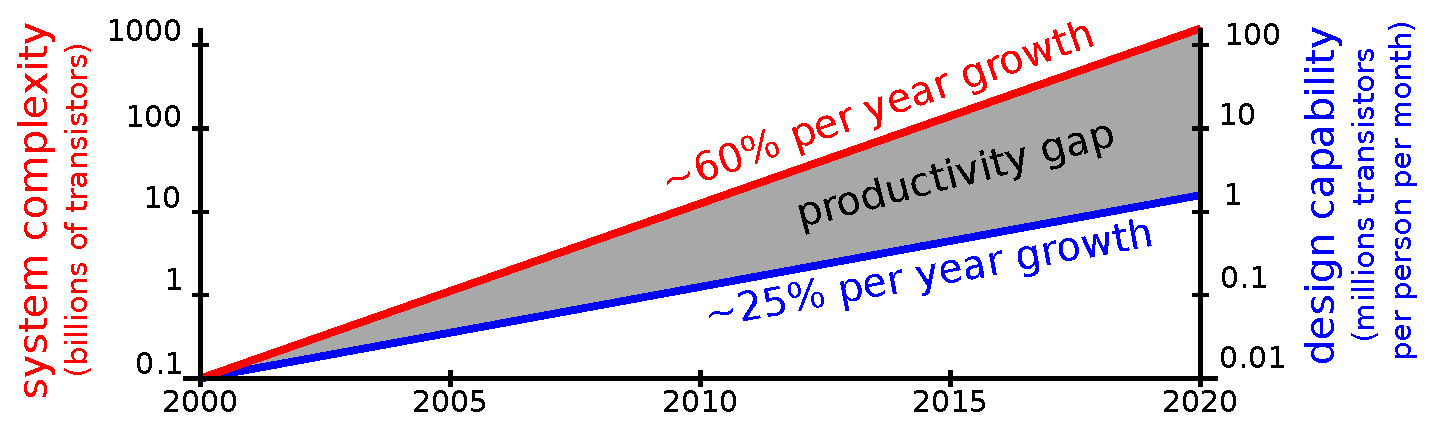
\includegraphics[scale=0.5]{fig/figs/productivity_gap}
   \caption{
     \label{fig:productivity_gap}
     Design productivity gap}
\end{figure}


% design reuse and need for async design principles
It has been predicted by ITRS~\cite{ITRS_2011} that in order to address the productivity gap challenge, by 2020 at least 90\% of the complex circuits should be built of previously designed components. This rises the need for compositional (or modular) design principles where the timing of individual modules is independent of the rest of the system and  therefore requires delay insensitive communication between the modules. This communication discipline is natural for asynchronous circuits where the data transfer is accompanied by request-acknowledgement handshaking between the sending and the receiving counterparts. On this pathway the previously designed Intellectual Property (IP) cores will need to be adapted to the new modular architectures. The least intrusive is the Globally Asynchronous Locally Synchronous (GALS) approach~\cite{Chapiro_1984_phd} where special wrappers~\cite{Mullins_2007_async, Fan_2009_iccd} are built around synchronous modules to convert their communication into asynchronous handshake style. Another alternative is desynchronisation techniques~\cite{Cortadella_2006_ieeetcad} where the global clock is replaced by a distributed control which determines when the computation is complete and the output result is ready to be consumed. This control may take different forms, from a delay line matching the critical path of the module~\cite{Cortadella_2010_icicdt} to explicitly introduced completion detection logic~\cite{Kondratyev_2002_ieeedtc}.

% synthesis of async components
The remaining 10\% of the IC components, as well as the interface and control logic to support the interconnect and communication flexibility, will still need to be designed from scratch. One way is to design those components in traditional synchronous way and then apply the previously discussed techniques to comply with the delay insensitive interface requirements. This, however, may result in suboptimal solutions in terms of circuit area, computation speed and energy consumption. Better results can be achieved if the components are designed and implemented with their asynchronous environment in mind~\cite{Martin_2006_ieeeproc}. However, the logic synthesis of asynchronous circuits is computationally expensive and not applicable to large modules. This is due to high level of concurrency in truly asynchronous systems which results in a state space explosion.  The computation complexity problem has been successfully addressed in the syntax-driven translation~\cite{balsa} approach which is based on direct mapping of a specification into hardware components without going through the state space exploration (it is assumed that there is one-to-one correspondence between the specification language constructs and the library of available components).

% need for compositional approach
The major drawback of the circuits obtained by the syntax-driven translation is the suboptimal performance of their control structures~\cite{Plana-balsa-control-overhead}. In order to resolve this issue the control models of all the components need to be composed together and resynthesised exploiting the benefits of their joint optimisation. Existing resynthesis methods are based on parallel composition of component models expressed in form of Petri nets~\cite{carmona-handshake-clustering}. However, the efficient parallel composition of the component models is still an open question and is one of the primary goals of this thesis.

\begin{figure}
\centering
   \newcommand{\figgg}[2]{
     \subfloat[#1]{
       \label{fig:#2}
       \includegraphics[scale=0.7]{fig/figs/#2}
   }}
   \figgg{Structural composition}{composition_structural}
   \\
   \figgg{Naive behavioural composition}{composition_behavioural_naive}
   \figgg{Behavioural composition}{composition_behavioural}
   \caption{
     \label{fig:composition_basics}
     Composition basics}
\end{figure}

% structural and behavioural aspects of composition
The composition of circuit components is of structural nature - they are combined via input-output interfaces according to the casual dependency between the operation they perform, as shown in Fig.~\ref{fig:composition_structural}.
Another compositional aspect is a combination of several mutually exclusive behaviours in the same circuit. A naive way to build such a circuit is to implement the different behaviour scenarious in separate modules and structurally compose them with the use of multiplexers and demultiplexers, as shown in Fig.~\ref{fig:composition_behavioural_naive}. A mode selection code on the (de)multiplexors determines the current scenario.  While this is a valid implementation of multi-modal functionality, it ignores the mutually exclusive feature of the implemented behaviours and ignores a possibility of partial hardware reuse for common functionality, as shown in Fig.~\ref{fig:composition_behavioural}.

A model which naturally captures the structural and behavioural aspects of composition in a single formalism is Conditional Partial Order Graphs (CPOGs)~\cite{2009_mokhov_phd}. This graph-based model is capable of expressing the structural composition by means of causality arcs (similar to Petri nets) and the behavioural composition by means of Boolean "visibility" conditions on its vertices. While CPOGs is a convenient tool for reasoning on small benchmarks, it lacks the means for capturing and transformation of large systems. The first  goal of this thesis is to generalise the CPOGs model and transition from the acyclic graphs representing partial orders into a universal Parameterised Graphs (PGs). The second goal is to introduce a theory for PG manipulation in algebraic form, which enables equivalence-preserving manipulation of graphs in symbolic form and simplifies specification and reasoning about complex systems.

The Boolean conditions on graph vertices can be expressed in various forms targeting different optimisation criteria. In the context of digital circuit design these conditions are subsequently implemented as the hardware control logic, therefore such optimisation targets as minimising the number of control variables and/or reducing the complexity of logical expressions, is of paramount importance. The ambitious goal of this thesis is to solve the optimisation problem for the general case, to express it in terms of Boolean satisfiability problem and to employ the existing SAT solving tools for obtaining the best result.


\section{Contributions}

The main contributions of the thesis are as follows:

\begin{itemize}
\item
\textbf{Improved parallel composition:} a novel method for composition of models specified with labelled Petri Nets.

\item
\textbf{PG theory:} CPOG generalisation to Parametrised Graph formalism and mechanised proof of its algebraic properties.

\item
\textbf{PG Synthesis:} a technique for synthesis of processor instruction decoder using instruction sets specified with Parametrised Graphs.

\item
\textbf{CAD tool support:} automation for the above, including improved parallel composition and encoding of TPG specifications using Workcraft framework.

\end{itemize}

\section{Overview}

Handshake circuits~\cite{van2004handshake} are widely applied in the design and synthesis of real-life hardware.
One prominent problem is obtaining an efficient implementation from a \emph{structural} compositional specification.
Syntax-based synthesis tools such as Balsa~\cite{balsa} are unable to take into account the compositional
behaviour of STGs corresponding to handshake circuit components. To address this issue we propose 
a technique that selectively composes STGs of related components to obtain a smaller and more performant
circuit without suffering state space explosion commonly associated with Petri net based techniques~\cite{Valmari}.
This transformation, which we refer to as \emph{resynthesis}~\cite{ukaf_balsa_resynthesis,CN-02,KVL-96,PC-96}, is accomplished in three stages. First, we apply a heuristic to identify the most promising candidates for STG-level composition. Second, we perform a parallel composition of the selected component STGs and as a result obtain a new handshake circuit with custom components, functionally equivalent to a combination of elementary components. Finally, a gate-level implementation is obtained from the new handshake circuit via a component-wise synthesis of STGs.

Unfortunately, the standard definition of parallel composition almost always yields a `messy' Petri net, with many implicit places, causing performance deterioration in techniques that are based on structural methods such as the resynthesis approach. To counter this, we propose an improved algorithm for computing the parallel composition. The algorithm generally produces nets with fewer implicit places that are better suited for subsequent application of structural methods~\cite{improved_par_comp}.

In addition to purely structural composition of STGs, it is also beneficial to consider a mixture of 
structural and behavioural composition. Conditional Partial Order Graphs (CPOG)~\cite{2009_mokhov_phd} is a graph-based notation supporting compact
representation and efficient manipulation of both structural and behavioural composition styles. As one example, when developing complex circuit, it is
often necessary to consider several operational modes of a circuit~\cite{2012_xia_iet,2012_mokhov_async}.
For this, one needs methodologies and tools to exploit similarities between
the individual modes and hence lift the level of discourse to behaviour families.
This necessitates that behaviours are managed in a compositional
way: the specification of the system must be composed from specifications
of its blocks. Furthermore, since the approach is intended to be a part of a safety critical toolchain, it is essential that such a  specification is amenable to mechanised reasoning and transformation.

In Chapter~\ref{chap:PGAlgebra} we propose an extension of the CPOG formalism, called Parameterised Graph (PG).
PGs deal with general graphs rather than just partial orders. We introduce an algebra of Parameterised Graphs by specifying the
equivalence relation via a set of axioms, which we prove to be sound,
minimal and complete~\cite{pg_algebra}. This result allows one to manipulate a PG model
as an algebraic expression applying the bi-directional rewrite rules of this algebra. This is  in contrast to the CPOG formalism that does not offer a unifying algebraic structure. We demonstrate
the usefulness of the developed formalism with two case studies coming
from the area of microelectronics design.

The CPOG formalism can be applied to merge several distinct behaviours
into a single compact CPOG~\cite{2009_mokhov_phd}. As one example, this has been previously used to
synthesise control logic for instruction decoding. In this thesis (Chapter~\ref{chap:PGEncoding}) 
we improve upon this work by offering a powerful technique to automatically discover an optimal encoding and
synthesise a matching optimal decoding circuit. From the outset, we consider a larger set of potential solutions
which enables us to formulate the global optimality criterion. We use an automated satisfiability solving 
techniques to find an optimal solution~\cite{cpog_encoding}.

\begin{figure}
\centering
   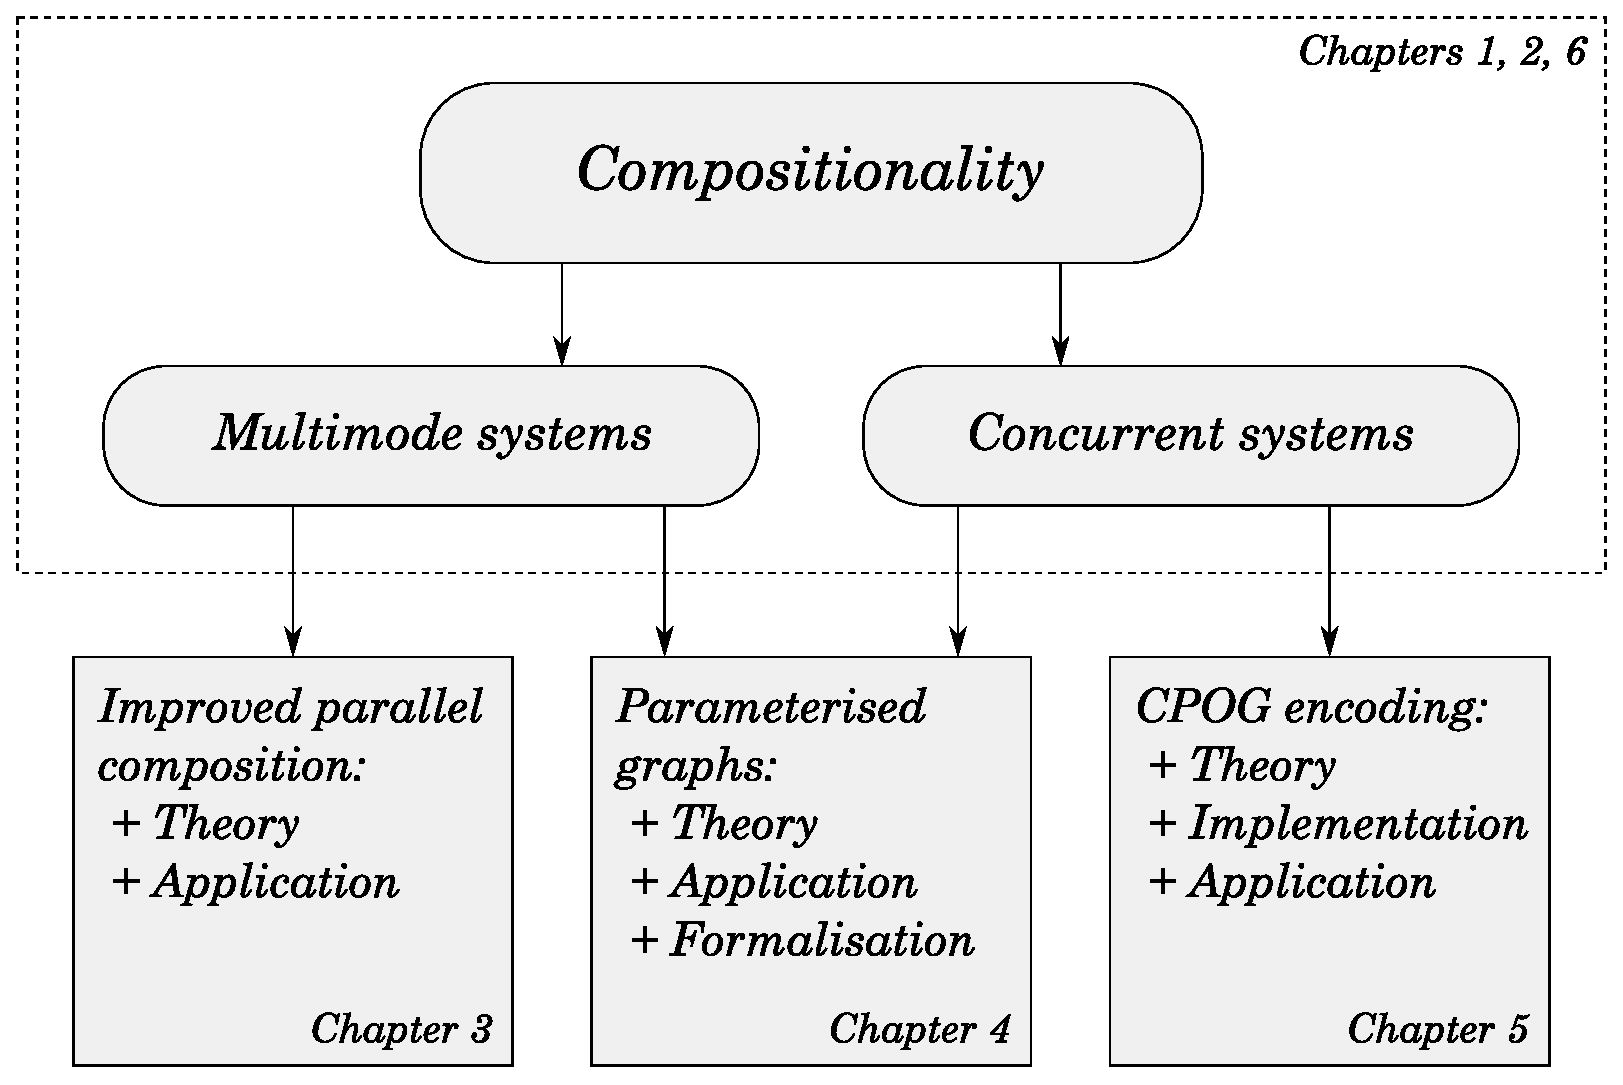
\includegraphics[scale=0.5]{fig/thesis}
   \caption{
     \label{fig:thesis_structure}
     Thesis structure}
\end{figure}

To summarize the thesis structure,

\begin{itemize}
\item
\textbf{Chapter~\ref{chap:Background}} covers the basics of handshake circuits, signal transition graphs and conditional partial order graphs.

\item
\textbf{Chapter~\ref{chap:ParComp}} describes the proposed improved parallel composition algorithm. The contents of this chapter is based on the results published previously in \cite{improved_par_comp}.

\item
\textbf{Chapter~\ref{chap:PGAlgebra}} introduces Parametrised Graph (PG) theory, defining and studying an algebraic structure that generalises Conditional Partial Order Graph formalism. This chapter is based on the results previously published in~\cite{pg_algebra}.

\item
\textbf{Chapter~\ref{chap:PGEncoding}} describes a technique for optimal encoding of processor instruction sets defined using PG formalism. This chapter is based on the results previously published in~\cite{cpog_encoding}. An earlier version of this paper has qualified for a Best Paper Award at the ACSD conference.

\item
\textbf{Chapter~\ref{chap:Conclusion}} summarises the achieved results and proposes ideas for future research.

\item
\textbf{Appendix} contains formal proofs in form of Agda source code for the PG Algebra properties discussed in Chapter~\ref{chap:PGAlgebra}.

\end{itemize}

The relationship between chapters is illustrated in Figure~\ref{fig:thesis_structure}.

\chapter{Background}

Background

\section{CSP}

\section{Handshake circuits}

\section{Petri Nets}\label{sec_pn_basic}

% ***************** Petri Net Basics ********************
A \emph{Petri net} is a 4-tuple $N=(P,T,W,M_N)$ where
$P$ is a finite set of \emph{places} and $T$ is a finite set of \emph{transitions}
with $P \cap T=\emptyset$,
$W: P\times T \cup T \times P \rightarrow \nat_0$ is the \emph{weight function,} and
$M_N$ is the \emph{initial marking}, where a \emph{marking} is a multiset of places,
\ie a function $P\rar\nat_0$ which assigns a number of \emph{tokens} to each place.
A Petri net can be considered as a bipartite graph with weighted arcs between places and transitions.
If necessary, we write $P_N$ etc.\ for the components of $N$ or $P'$ ($P_i$) etc.\ for the net $N'$ ($N_i$) etc.


% ***************** Preset, Postset ********************

The \emph{preset} of a place or transition $x$ is denoted as $\pre x$ and defined by
$\pre x\DEF\{y\in P\cup T\ |\  W(y,x)>0\}$,
the \emph{postset} of $x$ is denoted as $\post x$ and defined by
$\post x\DEF\{y\in P\cup T\ |\ W(x,y)>0\}$.
These notions are extended to sets as usual.
We say that there is an \emph{arc}
from each $y\in \pre x$ to~$x$.




% ***************** Enabledness, Reachable States ********************

A transition $t$ is \emph{enabled under a marking M}
if $\forall p\in \pre t:M(p)\geq W(p, t)$, which is denoted by $M\tfrs t$.
An enabled transition $t$ can \emph{fire} yielding a new marking $M'$,
written as $M\tfrs t M'$,
where $M'(p)=M(p)-W(p, t) + W(t,p)$, for all $p\in P$.
A transition sequence $\sigma=t_1\ldots t_n$ is \emph{enabled under a marking $M$} (yielding $M'$)
if $M\tfrs{t_1}M_1\tfrs{t_2}\ldots M_{n-1}\tfrs {t_n} M_n=M'$, and we
write $M\tfrs \sigma$, $M\tfrs \sigma M'$ resp.; $\sigma$ is called \emph{execution of $N$} if $M_N\tfrs \sigma$.
  The empty transition sequence $\lambda$ is  enabled under every marking.
$M$ is called \emph{reachable} if a transition sequence $\sigma$ with
$M_N\tfrs \sigma M$ exists.

$N$ is called \emph{bounded} if, for every reachable marking $M$ and every place $p$, $M(p)\leq k$ for some constant $k\in \nat$; if $k=1$, $N$ is called \emph{safe}. $N$ is bounded if and only if the set $\tfrs {M_N}$ of reachable markings is finite. In this thesis, we are mostly concerned with bounded Petri nets.

A place $p$ is \emph{implicit} if it can be deleted from the net
without changing the set of executions, and so an implicit place can be removed from the net without affecting its behaviour.\footnote{Note that an implicit place can cease to be implicit if another implicit place is removed first.}
Unfortunately, detecting
implicit places is expensive: the problem is \PSPACE-complete for safe and \EXPSPACE-complete for general Petri nets. A place $p$ is \emph{duplicate} if there is another place $p'$ with the same pre- and postsets whose initial marking does not exceed that of $p$. Duplicate places are implicit, and are cheap to detect.

\smallskip

An \emph{STG} is a tuple $N=(P,T,W,M_N,\I,\Ot,\ell)$ where
$(P,T,W,M_N)$ is a Petri net and $\I$ and $\Ot$  are disjoint
sets of \emph{input} and  \emph{output signals}. For
$\Sig=\I\cup\Ot$ being the set of all signals,
$\ell:T\rightarrow\Sig\times\{+,-\}\cup \{\lambda\}$ is the
\emph{labelling} function. $\Sig\times\{+,-\}$ or short
$\Sig\upd$ is the set of \emph{signal transitions}; its
elements are denoted  as $s^+$, $s^-$  resp.\ instead of
$(s,+)$, $(s,-)$ resp. A plus sign denotes that a signal value
changes from \emph{logical low} (written as 0) to \emph{logical
high} (written as 1), and a minus sign denotes the opposite
direction. We write $s\upd$ if it is not important or unknown
which direction takes place.

An STG can contain transitions labelled with $\lambda$, called
\emph{dummy} transitions, which do not correspond to any signal
change. \emph{Hiding a signal $s$} means to change the label of
all transitions labelled with $s\upd$ to $\lambda$. (The idea
of re-synthesis approach is to hide the signals used for
communication between components, which results in an STG with
fewer signals that often has a simpler implementation as a
circuit.) The labelling of an STG is called \emph{injective} if
for each pair of distinct non-dummy transitions $t$ and $t'$,
$\ell(t)\neq\ell(t')$.

\smallskip

Examples of STGs are shown in Figs.~\ref{fi-motivating-example1} and~\ref{fi-motivating-example2}.
Places are drawn as circles containing a number of tokens corresponding to the initial marking.
Unmarked places which have only one transition in their presets and postsets are
not drawn if the corresponding arcs have the weight~1; they are implicitly
given by an arc between these two transitions (and if such a place contains tokens, they are drawn on the arc itself). Transitions are drawn simply as their labels,
and the weight function is drawn as directed arcs $(x,y)$ whenever $W(x,y)\neq 0$ (and
labelled with $W(x,y)$ if $W(x,y)>1$).


\smallskip

% ********************** labels ***************************

We lift the notion of enabledness to transition labels: we write
$M\ifrs {\ell(t)}  M'$ if $M\tfrs t  M'$. This is extended to sequences
as usual -- deleting $\lambda$-labels automatically since $\lambda$
is the empty word; \ie $M\ifrs{s\upd}M'$ means that a sequence of
transitions fires, where one of them is labelled $s\upd$ while the
others (if any) are $\lambda$-labelled. A sequence
$\nu\in(\Sig\upd)^*$ is called a \emph{trace of a marking} $M$ if
$M\ifrs \nu$, and a \emph{trace} of $N$ if $M=M_N$. The \emph{language $L(N)$
of $N$} is the set of all traces of $N$.

\smallskip

The \emph{reachability graph} $\RG(N)$ of an STG $N$ is an arc-labelled
directed graph on the reachable markings of $N$ with $M_N$ as the root;
there is an arc from $M$ to $M'$ labelled $\ell(t)$ whenever
$M\tfrs {t} M'$. For bounded Petri nets and STGs, $\RG(N)$ can be seen as a finite automaton
(where all states are accepting), and $L(N)$ is the language of this
automaton.
Observe that automata with accepting states only can be
regarded as STGs (with the states as places, the initial state being the
only marked place, etc.); hence, all definitions for STGs also
apply to automata.

$N$ is \emph{deterministic} if $\RG(N)$
is a deterministic automaton: it contains no $\lambda$-labelled transitions
and there are no \emph{dynamic auto-conflicts,} \ie for each reachable marking $M$ and each signal transition $s\upd$
there is at most one $M'$ with $M \ifrs {s\upd} M'$. (Note that a deterministic STG
can have choices between different outputs, \eg an STG modelling
the standard arbiter is deterministic).

An STG with a set of all markings $S_2$ is said to \emph{simulate} another STG with 
a set of all markings $S_1$ iff there exist an 
$R \subset S_1 \times S_2$ such that $(M_{N 1},M_{N 2}) \in R$ and for any pair of markings 
$(M_1, M_2) \in R$, a label $l$ and a marking $M_1'$, $M_1\ifrs {l}  M_1'$ implies 
$M_2 \ifrs {l} M_2'$ for some $M_2'$. We call $R$ the witness of simulation. Now we can say that STGs $N_1$ and $N_2$ are \emph{bisimilar} iff $N_2$ simulates $N_1$ with witness $R$ and $N_2$ simulates $N_1$ with witness $R^{-1}$.

For deterministic STGs, language equivalence and bisimulation coincide, and the language can be taken as the semantics of such a specification. Unfortunately, the class of deterministic STGs is too restrictive in practice~\cite{KSV-08}, \eg:
\begin{itemize}
  \item using dummy transitions is often convenient in manual design;
  \item modelling OR-causality~\cite{ykklp96} as a safe STG requires non-determinism;
  \item hiding internal communication (and thus introducing dummy transitions) is a crucial step in re-synthesis.
\end{itemize}
Hence, one has to deal with non-deterministic STGs as well.

One might think that if $\RG(N)$ is non-deterministic, it can be \emph{determinised} (using well-known auto\-ma\-ta-the\-o\-re\-tic methods), \ie turned  into a language-equivalent deterministic
automaton with accepting states only; in particular, the resulting automaton will have no $\lambda$-arcs. Unfortunately, this is a bad idea, as shown in~\cite{KSV-08}, where the semantics of non-deterministic STGs was developed. It is based on the concept of \emph{output-determinacy,} which is a relaxation of determinism: An STG $N$ is \emph{output-determinate (OD)} if $M_N \ifrs {\nu}
M_1$ and $M_N \ifrs {\nu} M_2$ implies for every $x\in \Ot_N$ that
$M_1 \ifrs {x\upd}$ iff $M_2 \ifrs {x\upd}$.
It turns out that OD STGs are exactly the STGs which
have correct implementations according to the implementation relation introduced in~\cite{KSV-08}.
Hence, non-OD STGs are ill-formed, and in particular cannot be correctly implemented as
circuits. This shows that in general, \emph{the language is not a satisfactory semantics of
non-deterministic STGs;} in particular, \emph{synthesising the determinised reachability graph of a non-OD STG
will either fail or result in an incorrect circuit.} On the other hand, for the class of OD STGs~\cite{KSV-08} shows that their language
is an adequate semantics, and
implementation relation can be formulated purely in terms of the language.
An important property of OD STGs is that in them the enabledness of an output signal is a function of the trace, \ie given a trace $\nu$, the set of outputs by which $\nu$ can be extended is uniquely determined, even though there could be multiple executions corresponding to $\nu$.


\smallskip

In the following definition
of {\em parallel composition}~$\parallel$, see \eg~\cite{vowo02lncs}, we will have to
consider the distinction between input and output signals.
The idea of parallel composition is that the
composed systems run in parallel and synchronise on common actions
-- corresponding to circuits that are connected on the
wires corresponding to the signals.
Since a system controls its outputs, we cannot allow a signal to
be an output of more than one component; input signals, on the other
hand, can be shared.
An output signal of a component may be an input of
other components, and in any case it is an output of the composition.

The parallel composition of STGs $N_1$ and $N_2$ is defined if
$\Ot_1 \cap \Ot_2 = \emptyset$. If we drop this requirement, the
definition gives the {\em synchronous product} $N_1\times N_2$,
which is often useful. The place set of the composition is
the disjoint union of the place sets of the components; therefore,
we can consider markings of the composition (regarded as multisets)
as the disjoint union of markings of the components,
and we will also write such a marking $M_1 \dot{\cup} M_2$
of the composition as $(M_1, M_2)$. To define the transitions,  let
$A=(\I_1 \cup \Ot_1) \cap (\I_2 \cup \Ot_2)$ be the set of
common signals.
If \eg $s$ is an output of $N_1$ and an input of $N_2$,
then firing of $s\upd$ in $N_1$ is `seen' by
$N_2$, \ie it must be accompanied by firing of $s\upd$
in $N_2$. Since we do not know a priori which $s\upd$-labelled
transition of $N_2$ will fire together with some $s\upd$-labelled
transition of $N_1$, we have to allow for each possible
pairing.
Thus, the {\em parallel composition} $N = N_1 \parallel N_2$
is obtained from the disjoint union of $N_1$ and $N_2$ by
fusing
each $s\upd$-labelled transition $t_1$ of $N_1$
with each $s\upd$-labelled transition $t_2$ from $N_2$ if $s \in A$.
Such transitions are pairs and the firing $(M_1, M_2)\tfrs{(t_1,t_2) }(M_1', M_2')$ of $N$
corresponds to the firings $M_i\tfrs{t_i}M_i'$ in $N_i$, $i=1,2$; for an example
of a parallel composition, see Fig.~\ref{fig_parcom}.
More generally, we have $(M_1, M_2) \ifrs{\nu} (M_1', M_2')$ iff
$M_i \ifrs{\nu|_{N_i}} M_i'$ for  $i\in\{1,2\}$, where
$\nu|_{N_i}$ denotes the projection of the trace $\nu$ onto the signals of the STG ${N_i}$.
Hence, all reachable markings of $N$ have the form $(M_1, M_2)$,
where $M_i$ is a reachable marking of $N_i$, $i=1,2$.

Obviously, one can extend the notion of the parallel
composition to a finite family (or collection) $(C_i)_{i\in I}$ of
STGs as $\parallel_{i\in I} C_i$,
provided that no signal is an output signal of more than one of the
$C_i$. We will also denote the markings of such a composition
by $(M_1, \ldots,M_n)$ if $M_i$ is a marking of $C_i$ for
$i\in I=\{1,...,n\}$.
As above, $(M_1, M_2, \ldots, M_n) \ifrs{\nu} (M_1', M_2', \ldots, M_n')$ iff
$M_i \ifrs{\nu|_{C_i}} M_i'$ for all $i\in\{1,\ldots,n\}$.
It is easy to see that $C$ is deterministic if all $C_i$ are. However, this is not true for a composition of OD STGs, as the result, in general, can be non-OD in such a case.

A composition can also be ill-defined due to \emph{computation interference,} see \eg~\cite{eber92}.
Let $C\DEF\parallel_{i\in I}C_{i}$ be a composition of STGs. It is
\emph{free from computation interference (FCI)} if for every trace $\nu$ of $C$
the following holds: if $\nu|_{C_{j}}x^{\pm}$ is a trace of $C_{j}$
for some output $x$ of $C_{j}$, then $\nu|_{C}x^{\pm}$ is a trace
of $C$.

\begin{figure*}[t]
    \centering
    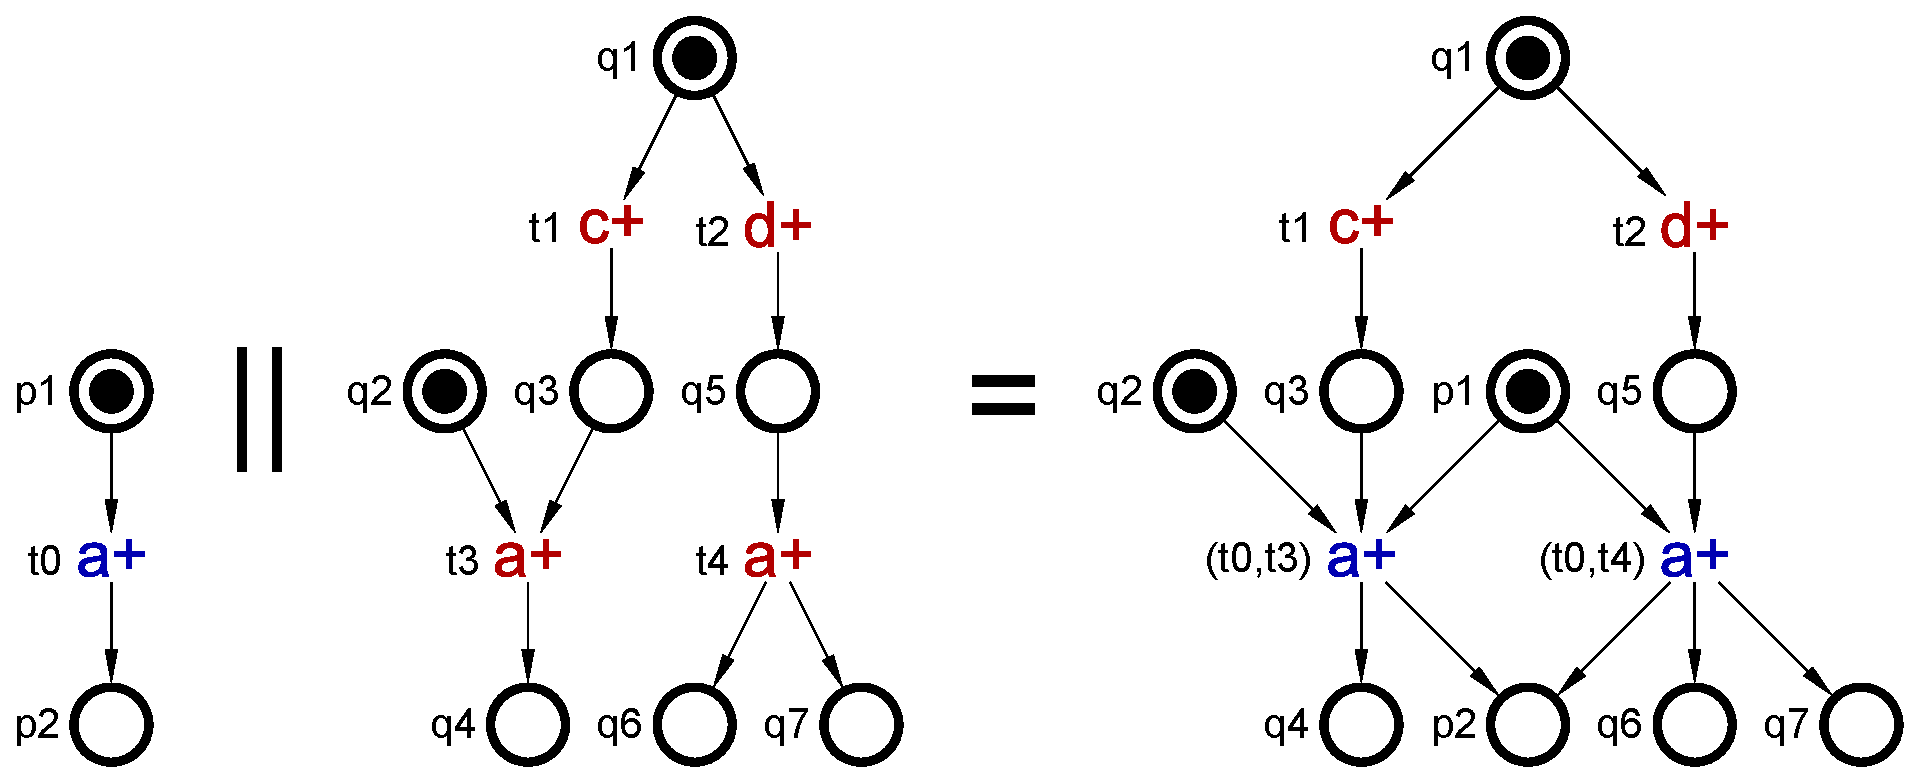
\includegraphics[scale=0.4]{EXPERIMENTS/stg/pcomp_example}
    \caption{\label{fig_parcom}
        Parallel composition example. In the net fragment on the left hand side,
        signal $a$ is an output, and in the fragment in the middle it is an input.
        Hence, in their parallel composition (right) it is an output.
        In this example, there is \emph{computation interference}: the left component activates $a\up$ but the middle one is not ready to receive it.}
\end{figure*}

\smallskip


\begin{figure*}[!tb]
    \centering
    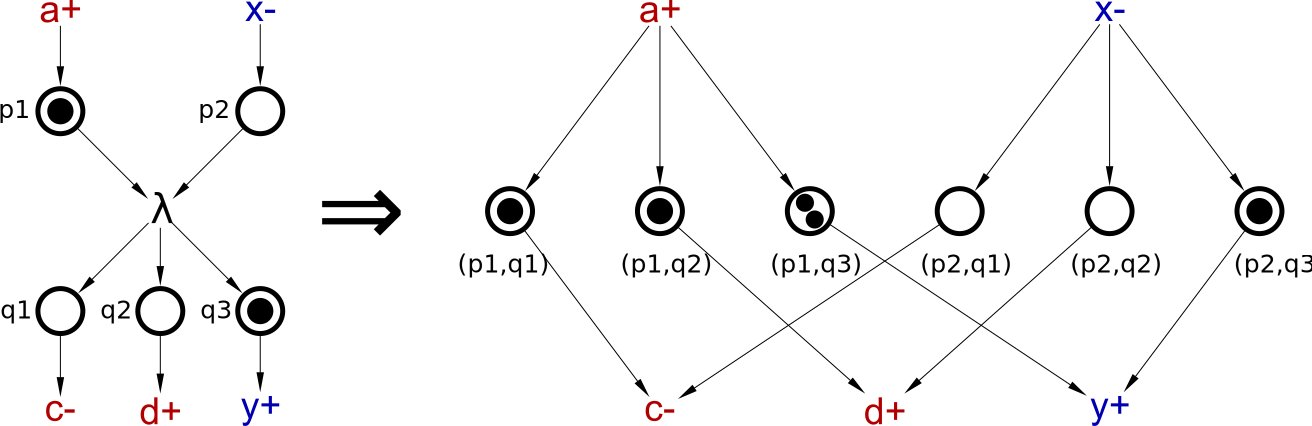
\includegraphics[scale=0.4]{EXPERIMENTS/stg/transition_contraction}
    \caption{\label{fig3.1}
        An example of a transition contraction.
    }
\end{figure*}


\emph{Transition contraction}~\cite{vowo02lncs} is an important operation in circuit re-synthesis. It removes a dummy transition from an STG and
combines each place of its preset with each place of its postset to `simulate' the
firing of the deleted transition, see Fig.~\ref{fig3.1}. Unfortunately, transition contractions are sometimes undefined (\eg in case the transition has a self-loop, \ie some place occurs in both its preset and postset); moreover, even when a contraction is defined, it might change the semantics of the STG.
Hence,~\cite{vowo02lncs} uses the notion of \emph{secure} contractions, that preserve the semantics.

Transition contractions preserve boundedness, but in general,
can turn a safe net into a non-safe one, as well as
introduce weighted arcs. In practice, it is often convenient to work with safe nets, and for this~\cite{KSVW-09} introduced \emph{safeness-preserving} contractions, \ie ones which
guarantee that  the transformed STG is safe if the initial one
was. (Note that the transitions with weighted arcs must be dead
in a safe Petri net, and so we can assume that the initial and
all the intermediate STGs contain no such arcs.) Also,~\cite{KSVW-09} developed a sufficient structural
condition for a contraction to be safe\-ness-pre\-ser\-ving.

From the point of view of this thesis, it is important to remark that implicit places can adversely affect the (secure) contractibility of a transition, \ie it is possible to have a situation when a transition is not contractible (or not securely contractible), but becomes securely contractible after some implicit place is removed from the STG. As detecting implicit places is expensive, it is very desirable to reduce their number by some other means, in particular the approach proposed in this thesis reduces the number of such places in STGs obtained by parallel composition. This has a direct effect on re-synthesis: if the composed STG has fewer implicit places, more dummy transitions in it can be contracted, and so it will be easier to synthesise the result.


\section{PG Encoding}

\subsection{Abstract}
There is a critical need for design automation in microarchitectural
modelling and synthesis. One of the areas which lacks the necessary
automation support is synthesis of instruction codes targeting various
design optimality criteria. This paper aims to fill this gap by providing
a set of formal methods and a software tool for synthesis of instruction
codes given the description of a processor as a set of instructions.

The method is based on the Conditional Partial Order Graph (CPOG)
model introduced recently, which is a formalism for efficient specification
and synthesis of microcontrol circuits. It describes a system as a
functional composition of its behavioural scenarios, or instructions,
each of them being a partial order of events. In order to distinguish
instructions within a CPOG they are given different encodings represented
with Boolean vectors. Size and latency of the final microcontroller
significantly depends on the chosen encodings, thus efficient synthesis
of instruction codes is essential.

The paper shows that the CPOG model is a very convenient formalism
for efficient representation of processor instruction sets. It provides
a ground for a concise formulation of several encoding problems, which
are reducible to the well-known Boolean satisfiability (SAT) problem
and can be efficiently solved by modern SAT solvers. Application of
all the presented techniques is demonstrated on a processor design
example.

\subsection{Introduction}

Automated design of general purpose processing cores, application-specific
instruction-set processors (ASIPs), and distributed Systems-on-Chip
(SoCs) has gained a lot of attention from academia and industry~\cite{2006_dutt_chapter}.
New formalisms for data-path modelling are proposed~\cite{2010_mokhov_ieee}\cite{2008_sokolov_sdfs},
hardware/software co-design methodology~\cite{1993_alomary_edac}
is actively developed and applied for ASIP performance improvement,
more specific techniques (such as compiler-directed instruction set
optimisation~\cite{2002_qin_date}) are constantly introduced into
the instruction set architecture (ISA) design domain.

\begin{figure}
\begin{centering}
\vspace{-3mm}
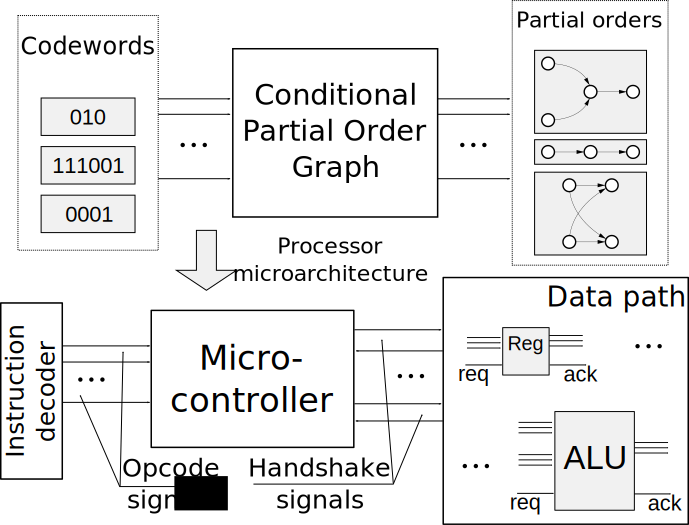
\includegraphics[width=0.6\columnwidth]{fig/control}\vspace{-1mm}

\par\end{centering}

\caption{CPOGs and processor microcontrol\label{fig:Dynamically-reconfigurable-controller}}
\vspace{-3mm}
\end{figure}


Synthesis of instruction sets is a particularly active research area.
There are methods for automated ISA synthesis for a target platform
(according to available system resources and data-path components)
and for given software requirements (e.g. aimed to ease compilation
or reduce program length). These methods eventually produce a structured
set of instructions satisfying certain properties (orthogonality,
completeness, regularity, etc.); instructions are grouped into classes
and each class is allocated a certain opcode interval within the total
code space~\cite{2003_nohl_dac}. At this point automation is typically
stopped or becomes trivial: the instructions are given arbitrary codes
within the allocated intervals. This limits performance due to instruction
decoder circuitry overheads. The problem is usually approached by
ad-hoc heuristics or application-specific optimisation techniques
(see, for example,~\cite{2002_lee_iccad}).

In this paper we try to solve the general problem of optimal encoding
of a given set of instructions with the aid of the Conditional Partial
Order Graph (CPOG) model introduced recently~\cite{2009_mokhov_phd}\cite{2010_mokhov_ieee}.
The key features of the model are: ability to describe systems in
a compact functional form, and structural synthesis methods which
significantly improve performance of the whole design flow. These
features make the model very efficient for representation and management
of processor instruction sets in hardware and EDA software. A CPOG
is a superposition of a set of partial orders which can be extracted
from it by providing the corresponding codewords, see Figure~\ref{fig:Dynamically-reconfigurable-controller}
(top). It can be regarded as a custom associative memory for storing
cause and effect relations within a predefined set of events.

There are different kinds of systems which can be described with the
model. For example, a processor microcontroller executes partial orders
(or \textbf{instructions}) of primitive computational steps (or \textbf{microinstructions})
defined on a set of data path operational units, see Figure~\ref{fig:Dynamically-reconfigurable-controller}
(bottom). The order is determined by an \textbf{instruction}\textbf{\emph{
}}\textbf{code} --- a combination of logical conditions presented
to the controller by the environment~\cite{1994_de_micheli_book}.
To this end, the microcontroller can be seen as an entity which communicates
with two parts of the environment: one part is the source of condition
signals (an instruction decoder) and the other part is a set of controlled
objects with request-acknowledgement interface (data path operational
units which execute the microinstructions).

There are many criteria which determine the choice of a particular
processor architecture and influence design of an instruction set:
functionality, operation modes, resources, etc. In Section~\ref{sec-processor}
we study an example of an instruction set (a subset of \emph{MSP430}
processor~\cite{mspmanual}) implemented on a minimalistic hardware
platform. However, the main focus of this paper is optimal encoding
of processor instruction sets in the general architecture-independent
context. See~\cite{2011_mokhov_tr} for investigation of the architecture-level
reasoning using the CPOG model.

Main contributions of this paper are: firstly, it formulates several
instruction set encoding problems in terms of the CPOG model; secondly,
it presents the SAT characterisation of the problems leading to their
efficient automated solution; thirdly, it demonstrates application
of the CPOG methodology at different stages of a processor design
flow --- from architectural-level specification, design and behavioural
description of an instruction set to its encoding and synthesis of
the physical implementation of the microcontroller. The paper is organised
as follows. Section~\ref{sec:CPOG-model-essentials} briefly introduces
the CPOG model providing a ground for formulating a set of problems
of optimal instruction set encoding in Section~\ref{sec:Optimal-encoding-problem}.
A method for automated translation of the problems into SAT instances
is explained in Section~\ref{sec:SAT-formulation}. It is followed
by a processor design example in Section~\ref{sec-processor} and
conclusions.


\section{Conclusions}

\chapter{Approach}



Handshake circuits are widely applied in the design and synthesis of real-life hardware.
One prominent problem is obtaining an efficient implementation from a \emph{structural} compositional specification.
Syntax-based synthesis tools such as Balsa~\cite{balsa} are unable to take into account the compositional
behaviour of STGs corresponding to handshake circuit components. To address this issue we propose 
a technique that selectively composes STGs of related components to obtain a smaller and more performant
circuit without suffering state space explosion commonly associated with Petri net based techniques~\cite{Valmari}.
This transformation, which we refer to as \emph{resynthesis}~\cite{ukaf_balsa_resynthesis}, is done in three stages. First, we apply a heuristic to identify the most promising candidates for STG-level composition. Second, we perform a parallel composition of the selected component STGs and as a result obtain a new handshake circuit with custom components. Finally, a gate-level implementation is obtained from the new handshake circuit via a component-wise synthesis of STGs.

Unfortunately, the standard definition of parallel composition almost always yields a `messy' Petri net, with many implicit places, causing performance deterioration in techniques that are based on structural methods such as the resynthesis approach. To counter this, we propose an improved algorithm for computing the parallel composition. The algorithm generally produces nets with fewer implicit places that are better suited for subsequent application of structural methods~\cite{improved_par_comp}.

In addition to purely structural composition of STGs, it is also beneficial to consider a mixture of 
structural and behavioural composition. CPOG~\cite{2009_mokhov_phd} is a graph-based notation supporting compact
representation and efficient manipulation of the two forms of composition. As one example, it is
often necessary to consider several operational modes of a circuit. 
For this, one needs methodologies and tools to exploit similarities between
the individual modes and hence lift the level of discourse to behaviour families.
This necessitates that behaviours are managed in a compositional
way: the specification of the system must be composed from specifications
of its blocks. Furthermore, since the approach is intended to be a part of a safety critical toolchain, it is essential that such a  specification is amenable to mechanised reasoning and transformation.

In Chapter~\ref{chap:agda} we propose an extension of the CPOG formalism, called Parameterised Graph (PG).
PGs deal with general graphs rather than just partial orders. We introduce an algebra of Parameterised Graphs by specifying the
equivalence relation by a set of axioms, which is proved to be sound,
minimal and complete~\cite{pg_algebra}. This allows one to manipulate the specifications
as algebraic expressions using the rules of this algebra in contrast to the CPOG that does not offer a unifying algebraic structure. We demonstrate
the usefulness of the developed formalism on two case studies coming
from the area of microelectronics design.

The CPOG formalism can be applied to merge several distinct behaviours
into a single compact CPOG~\cite{2009_mokhov_phd}. As one example, this has been previously used to
synthesise control logic for instruction decoding. In this thesis (Chapter~\ref{chap:pg_encoding}) 
we improve upon this work by offering a powerful technique to automatically discover an optimal encoding and
synthesise a matching optimal decoding circuit. From the outset, we consider a larger set of potential solutions
which enables us to formulate the global optimality criterion. We use an automated satisfiability solving 
techniques to find an optimal solution~\cite{pg_encoding}.




* Improved parallel composition
* PG Algebra
* PG Encoding

\subsection{Abstract of Balsa Resynthesis}

The controllers obtained
by syntax-directed mapping used in Balsa usually suffer from performance,
area and power overheads because the predesigned set of components
is required to implement the declared protocols fully and correctly
in order to be reusable in all possible circuit configurations, which
results in redundancy. This redundancy can be eliminated by replacing
the manually designed gate-level implementations of the high level
components with the corresponding STG specifications. The STGs of
individual components that form the system are then composed together
to produce the final system STG that is used to synthesise an optimal
implementation of the control circuit. The process is automated as
a plug-in for Workcraft framework.

\subsection{Introduction of Balsa Resynthesis\label{sec:Balsa-Introduction}}

The main obstacle for the wider spread of asynchronous systems remains
to be the inherent complexity of their design. Several solutions are
accepted by the industry that ease the design process through abstraction
of predesigned asynchronous circuit parts as standardised high level
components. A designer is able to use these components as ``building
blocks'', and then obtain the final gate-level design through an
automated mapping process. Furthermore, some of the well-known asynchronous
design automation packages, such as Tangram~\cite{951597}, and Balsa~\cite{balsa},
define a high-level programming-like language that is used to describe
systems. The language constructs are then directly translated into
a network of \emph{handshake components }-- blocks with predefined
functionality that use \emph{handshakes} to interface with other components,
which are in turn mapped into a gate netlist. 

Although this method greatly enhances the designer's productivity,
it has several important drawbacks, of which the control-path overhead
is the most decisive. The controllers obtained by syntax-directed
mapping are usually far from optimal, because the predesigned components
are required to implement their declared protocols fully and correctly
in order to be reusable in all possible circuit configurations. However,
it is often the case that a significant part of their functionality
becomes redundant due to the peculiarities of the specific configuration,
e.g. in many cases full handshaking between the components can be
avoided.

This redundancy can be eliminated by replacing the manually designed
gate-level implementation of the high level components with an equivalent
STG~(signal transition graph)~\cite{Yakovlev_1998_cs} specification.
The individual component STGs are then composed together to form a
complete system STG~\cite{785214}, which is optimised using \noun{petrify~}\cite{cortadella_petrify}\noun{.}
An optimal gate-level implementation can then be automatically produced
from the STG using tools such as \noun{petrify}~\noun{\cite{cortadella_petrify},
SIS}~\cite{Sentovich:M92/41}\noun{ }and\noun{ MPSat}~\cite{Khomenko_2004_MPSAT}\noun{.}
Automatic synthesis becomes problematic when the size of the STG becomes
large: modern synthesis tools can handle STGs of no more than 100
signals. The impact of this problem can be lessened by including STG
decomposition tools~\cite{DesiJ} into the workflow, that would break
the large optimised STG down into several smaller STGs that are synthesisable
in reasonable time. Alternatively, the decomposition step can be carried
out on the level of the handshake circuits, dividing the circuit into
smaller blocks of components.

This section proposes an automated method to include the aforementioned
modification of the standard design workflow that is used in Balsa
design automation system~\cite{balsa} using \noun{Workcraft~\cite{DBLP:conf/apn/PoliakovKY09}
}framework.


\section{Petri Nets}\label{sec_pn_basic}

% ***************** Petri Net Basics ********************
A \emph{Petri net} is a 4-tuple $N=(P,T,W,M_N)$ where
$P$ is a finite set of \emph{places} and $T$ is a finite set of \emph{transitions}
with $P \cap T=\emptyset$,
$W: P\times T \cup T \times P \rightarrow \nat_0$ is the \emph{weight function,} and
$M_N$ is the \emph{initial marking}, where a \emph{marking} is a multiset of places,
\ie a function $P\rar\nat_0$ which assigns a number of \emph{tokens} to each place.
A Petri net can be considered as a bipartite graph with weighted arcs between places and transitions.
If necessary, we write $P_N$ etc.\ for the components of $N$ or $P'$ ($P_i$) etc.\ for the net $N'$ ($N_i$) etc.


% ***************** Preset, Postset ********************

The \emph{preset} of a place or transition $x$ is denoted as $\pre x$ and defined by
$\pre x\DEF\{y\in P\cup T\ |\  W(y,x)>0\}$,
the \emph{postset} of $x$ is denoted as $\post x$ and defined by
$\post x\DEF\{y\in P\cup T\ |\ W(x,y)>0\}$.
These notions are extended to sets as usual.
We say that there is an \emph{arc}
from each $y\in \pre x$ to~$x$.




% ***************** Enabledness, Reachable States ********************

A transition $t$ is \emph{enabled under a marking M}
if $\forall p\in \pre t:M(p)\geq W(p, t)$, which is denoted by $M\tfrs t$.
An enabled transition $t$ can \emph{fire} yielding a new marking $M'$,
written as $M\tfrs t M'$,
where $M'(p)=M(p)-W(p, t) + W(t,p)$, for all $p\in P$.
A transition sequence $\sigma=t_1\ldots t_n$ is \emph{enabled under a marking $M$} (yielding $M'$)
if $M\tfrs{t_1}M_1\tfrs{t_2}\ldots M_{n-1}\tfrs {t_n} M_n=M'$, and we
write $M\tfrs \sigma$, $M\tfrs \sigma M'$ resp.; $\sigma$ is called \emph{execution of $N$} if $M_N\tfrs \sigma$.
  The empty transition sequence $\lambda$ is  enabled under every marking.
$M$ is called \emph{reachable} if a transition sequence $\sigma$ with
$M_N\tfrs \sigma M$ exists.

$N$ is called \emph{bounded} if, for every reachable marking $M$ and every place $p$, $M(p)\leq k$ for some constant $k\in \nat$; if $k=1$, $N$ is called \emph{safe}. $N$ is bounded if and only if the set $\tfrs {M_N}$ of reachable markings is finite. In this thesis, we are mostly concerned with bounded Petri nets.

A place $p$ is \emph{implicit} if it can be deleted from the net
without changing the set of executions, and so an implicit place can be removed from the net without affecting its behaviour.\footnote{Note that an implicit place can cease to be implicit if another implicit place is removed first.}
Unfortunately, detecting
implicit places is expensive: the problem is \PSPACE-complete for safe and \EXPSPACE-complete for general Petri nets. A place $p$ is \emph{duplicate} if there is another place $p'$ with the same pre- and postsets whose initial marking does not exceed that of $p$. Duplicate places are implicit, and are cheap to detect.

\smallskip

An \emph{STG} is a tuple $N=(P,T,W,M_N,\I,\Ot,\ell)$ where
$(P,T,W,M_N)$ is a Petri net and $\I$ and $\Ot$  are disjoint
sets of \emph{input} and  \emph{output signals}. For
$\Sig=\I\cup\Ot$ being the set of all signals,
$\ell:T\rightarrow\Sig\times\{+,-\}\cup \{\lambda\}$ is the
\emph{labelling} function. $\Sig\times\{+,-\}$ or short
$\Sig\upd$ is the set of \emph{signal transitions}; its
elements are denoted  as $s^+$, $s^-$  resp.\ instead of
$(s,+)$, $(s,-)$ resp. A plus sign denotes that a signal value
changes from \emph{logical low} (written as 0) to \emph{logical
high} (written as 1), and a minus sign denotes the opposite
direction. We write $s\upd$ if it is not important or unknown
which direction takes place.

An STG can contain transitions labelled with $\lambda$, called
\emph{dummy} transitions, which do not correspond to any signal
change. \emph{Hiding a signal $s$} means to change the label of
all transitions labelled with $s\upd$ to $\lambda$. (The idea
of re-synthesis approach is to hide the signals used for
communication between components, which results in an STG with
fewer signals that often has a simpler implementation as a
circuit.) The labelling of an STG is called \emph{injective} if
for each pair of distinct non-dummy transitions $t$ and $t'$,
$\ell(t)\neq\ell(t')$.

\smallskip

Examples of STGs are shown in Figs.~\ref{fi-motivating-example1} and~\ref{fi-motivating-example2}.
Places are drawn as circles containing a number of tokens corresponding to the initial marking.
Unmarked places which have only one transition in their presets and postsets are
not drawn if the corresponding arcs have the weight~1; they are implicitly
given by an arc between these two transitions (and if such a place contains tokens, they are drawn on the arc itself). Transitions are drawn simply as their labels,
and the weight function is drawn as directed arcs $(x,y)$ whenever $W(x,y)\neq 0$ (and
labelled with $W(x,y)$ if $W(x,y)>1$).


\smallskip

% ********************** labels ***************************

We lift the notion of enabledness to transition labels: we write
$M\ifrs {\ell(t)}  M'$ if $M\tfrs t  M'$. This is extended to sequences
as usual -- deleting $\lambda$-labels automatically since $\lambda$
is the empty word; \ie $M\ifrs{s\upd}M'$ means that a sequence of
transitions fires, where one of them is labelled $s\upd$ while the
others (if any) are $\lambda$-labelled. A sequence
$\nu\in(\Sig\upd)^*$ is called a \emph{trace of a marking} $M$ if
$M\ifrs \nu$, and a \emph{trace} of $N$ if $M=M_N$. The \emph{language $L(N)$
of $N$} is the set of all traces of $N$.

\smallskip

The \emph{reachability graph} $\RG(N)$ of an STG $N$ is an arc-labelled
directed graph on the reachable markings of $N$ with $M_N$ as the root;
there is an arc from $M$ to $M'$ labelled $\ell(t)$ whenever
$M\tfrs {t} M'$. For bounded Petri nets and STGs, $\RG(N)$ can be seen as a finite automaton
(where all states are accepting), and $L(N)$ is the language of this
automaton.
Observe that automata with accepting states only can be
regarded as STGs (with the states as places, the initial state being the
only marked place, etc.); hence, all definitions for STGs also
apply to automata.

$N$ is \emph{deterministic} if $\RG(N)$
is a deterministic automaton: it contains no $\lambda$-labelled transitions
and there are no \emph{dynamic auto-conflicts,} \ie for each reachable marking $M$ and each signal transition $s\upd$
there is at most one $M'$ with $M \ifrs {s\upd} M'$. (Note that a deterministic STG
can have choices between different outputs, \eg an STG modelling
the standard arbiter is deterministic).

An STG with a set of all markings $S_2$ is said to \emph{simulate} another STG with 
a set of all markings $S_1$ iff there exist an 
$R \subset S_1 \times S_2$ such that $(M_{N 1},M_{N 2}) \in R$ and for any pair of markings 
$(M_1, M_2) \in R$, a label $l$ and a marking $M_1'$, $M_1\ifrs {l}  M_1'$ implies 
$M_2 \ifrs {l} M_2'$ for some $M_2'$. We call $R$ the witness of simulation. Now we can say that STGs $N_1$ and $N_2$ are \emph{bisimilar} iff $N_2$ simulates $N_1$ with witness $R$ and $N_2$ simulates $N_1$ with witness $R^{-1}$.

For deterministic STGs, language equivalence and bisimulation coincide, and the language can be taken as the semantics of such a specification. Unfortunately, the class of deterministic STGs is too restrictive in practice~\cite{KSV-08}, \eg:
\begin{itemize}
  \item using dummy transitions is often convenient in manual design;
  \item modelling OR-causality~\cite{ykklp96} as a safe STG requires non-determinism;
  \item hiding internal communication (and thus introducing dummy transitions) is a crucial step in re-synthesis.
\end{itemize}
Hence, one has to deal with non-deterministic STGs as well.

One might think that if $\RG(N)$ is non-deterministic, it can be \emph{determinised} (using well-known auto\-ma\-ta-the\-o\-re\-tic methods), \ie turned  into a language-equivalent deterministic
automaton with accepting states only; in particular, the resulting automaton will have no $\lambda$-arcs. Unfortunately, this is a bad idea, as shown in~\cite{KSV-08}, where the semantics of non-deterministic STGs was developed. It is based on the concept of \emph{output-determinacy,} which is a relaxation of determinism: An STG $N$ is \emph{output-determinate (OD)} if $M_N \ifrs {\nu}
M_1$ and $M_N \ifrs {\nu} M_2$ implies for every $x\in \Ot_N$ that
$M_1 \ifrs {x\upd}$ iff $M_2 \ifrs {x\upd}$.
It turns out that OD STGs are exactly the STGs which
have correct implementations according to the implementation relation introduced in~\cite{KSV-08}.
Hence, non-OD STGs are ill-formed, and in particular cannot be correctly implemented as
circuits. This shows that in general, \emph{the language is not a satisfactory semantics of
non-deterministic STGs;} in particular, \emph{synthesising the determinised reachability graph of a non-OD STG
will either fail or result in an incorrect circuit.} On the other hand, for the class of OD STGs~\cite{KSV-08} shows that their language
is an adequate semantics, and
implementation relation can be formulated purely in terms of the language.
An important property of OD STGs is that in them the enabledness of an output signal is a function of the trace, \ie given a trace $\nu$, the set of outputs by which $\nu$ can be extended is uniquely determined, even though there could be multiple executions corresponding to $\nu$.


\smallskip

In the following definition
of {\em parallel composition}~$\parallel$, see \eg~\cite{vowo02lncs}, we will have to
consider the distinction between input and output signals.
The idea of parallel composition is that the
composed systems run in parallel and synchronise on common actions
-- corresponding to circuits that are connected on the
wires corresponding to the signals.
Since a system controls its outputs, we cannot allow a signal to
be an output of more than one component; input signals, on the other
hand, can be shared.
An output signal of a component may be an input of
other components, and in any case it is an output of the composition.

The parallel composition of STGs $N_1$ and $N_2$ is defined if
$\Ot_1 \cap \Ot_2 = \emptyset$. If we drop this requirement, the
definition gives the {\em synchronous product} $N_1\times N_2$,
which is often useful. The place set of the composition is
the disjoint union of the place sets of the components; therefore,
we can consider markings of the composition (regarded as multisets)
as the disjoint union of markings of the components,
and we will also write such a marking $M_1 \dot{\cup} M_2$
of the composition as $(M_1, M_2)$. To define the transitions,  let
$A=(\I_1 \cup \Ot_1) \cap (\I_2 \cup \Ot_2)$ be the set of
common signals.
If \eg $s$ is an output of $N_1$ and an input of $N_2$,
then firing of $s\upd$ in $N_1$ is `seen' by
$N_2$, \ie it must be accompanied by firing of $s\upd$
in $N_2$. Since we do not know a priori which $s\upd$-labelled
transition of $N_2$ will fire together with some $s\upd$-labelled
transition of $N_1$, we have to allow for each possible
pairing.
Thus, the {\em parallel composition} $N = N_1 \parallel N_2$
is obtained from the disjoint union of $N_1$ and $N_2$ by
fusing
each $s\upd$-labelled transition $t_1$ of $N_1$
with each $s\upd$-labelled transition $t_2$ from $N_2$ if $s \in A$.
Such transitions are pairs and the firing $(M_1, M_2)\tfrs{(t_1,t_2) }(M_1', M_2')$ of $N$
corresponds to the firings $M_i\tfrs{t_i}M_i'$ in $N_i$, $i=1,2$; for an example
of a parallel composition, see Fig.~\ref{fig_parcom}.
More generally, we have $(M_1, M_2) \ifrs{\nu} (M_1', M_2')$ iff
$M_i \ifrs{\nu|_{N_i}} M_i'$ for  $i\in\{1,2\}$, where
$\nu|_{N_i}$ denotes the projection of the trace $\nu$ onto the signals of the STG ${N_i}$.
Hence, all reachable markings of $N$ have the form $(M_1, M_2)$,
where $M_i$ is a reachable marking of $N_i$, $i=1,2$.

Obviously, one can extend the notion of the parallel
composition to a finite family (or collection) $(C_i)_{i\in I}$ of
STGs as $\parallel_{i\in I} C_i$,
provided that no signal is an output signal of more than one of the
$C_i$. We will also denote the markings of such a composition
by $(M_1, \ldots,M_n)$ if $M_i$ is a marking of $C_i$ for
$i\in I=\{1,...,n\}$.
As above, $(M_1, M_2, \ldots, M_n) \ifrs{\nu} (M_1', M_2', \ldots, M_n')$ iff
$M_i \ifrs{\nu|_{C_i}} M_i'$ for all $i\in\{1,\ldots,n\}$.
It is easy to see that $C$ is deterministic if all $C_i$ are. However, this is not true for a composition of OD STGs, as the result, in general, can be non-OD in such a case.

A composition can also be ill-defined due to \emph{computation interference,} see \eg~\cite{eber92}.
Let $C\DEF\parallel_{i\in I}C_{i}$ be a composition of STGs. It is
\emph{free from computation interference (FCI)} if for every trace $\nu$ of $C$
the following holds: if $\nu|_{C_{j}}x^{\pm}$ is a trace of $C_{j}$
for some output $x$ of $C_{j}$, then $\nu|_{C}x^{\pm}$ is a trace
of $C$.

\begin{figure*}[t]
    \centering
    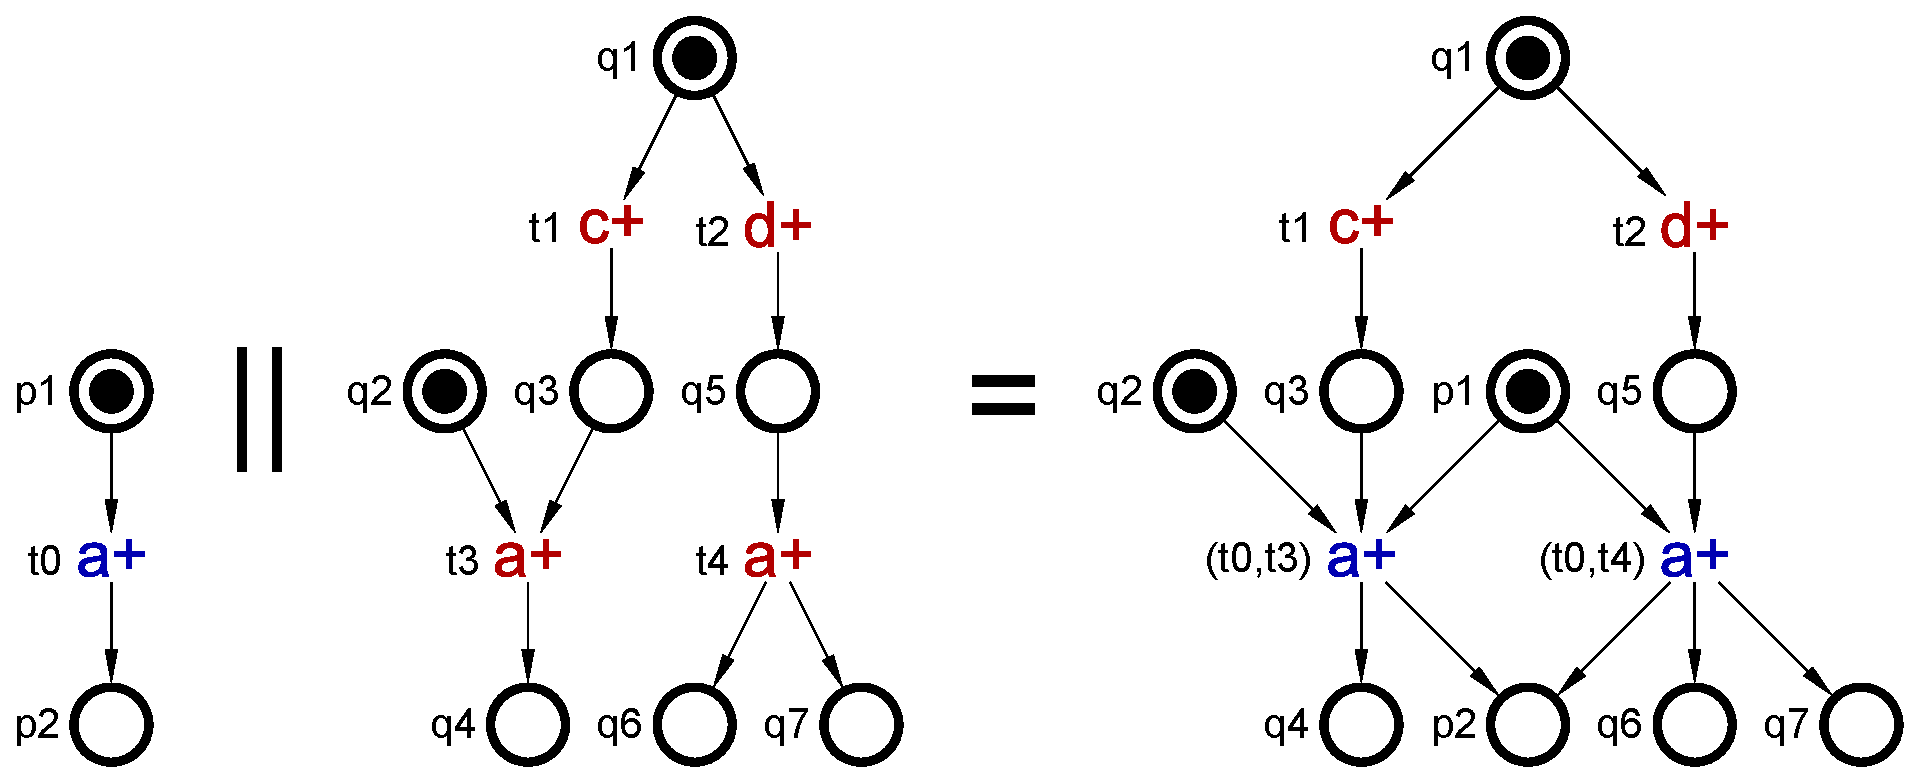
\includegraphics[scale=0.4]{EXPERIMENTS/stg/pcomp_example}
    \caption{\label{fig_parcom}
        Parallel composition example. In the net fragment on the left hand side,
        signal $a$ is an output, and in the fragment in the middle it is an input.
        Hence, in their parallel composition (right) it is an output.
        In this example, there is \emph{computation interference}: the left component activates $a\up$ but the middle one is not ready to receive it.}
\end{figure*}

\smallskip


\begin{figure*}[!tb]
    \centering
    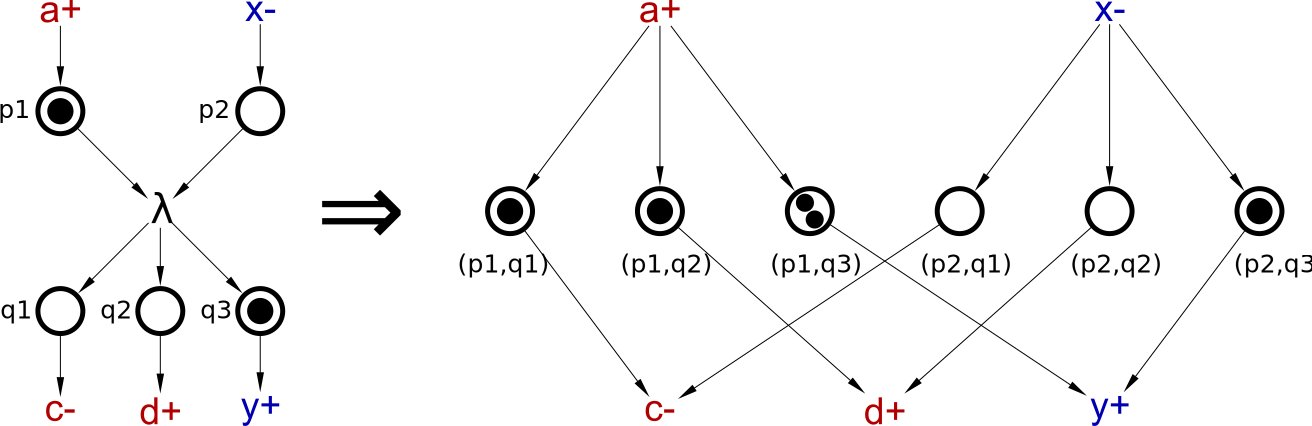
\includegraphics[scale=0.4]{EXPERIMENTS/stg/transition_contraction}
    \caption{\label{fig3.1}
        An example of a transition contraction.
    }
\end{figure*}


\emph{Transition contraction}~\cite{vowo02lncs} is an important operation in circuit re-synthesis. It removes a dummy transition from an STG and
combines each place of its preset with each place of its postset to `simulate' the
firing of the deleted transition, see Fig.~\ref{fig3.1}. Unfortunately, transition contractions are sometimes undefined (\eg in case the transition has a self-loop, \ie some place occurs in both its preset and postset); moreover, even when a contraction is defined, it might change the semantics of the STG.
Hence,~\cite{vowo02lncs} uses the notion of \emph{secure} contractions, that preserve the semantics.

Transition contractions preserve boundedness, but in general,
can turn a safe net into a non-safe one, as well as
introduce weighted arcs. In practice, it is often convenient to work with safe nets, and for this~\cite{KSVW-09} introduced \emph{safeness-preserving} contractions, \ie ones which
guarantee that  the transformed STG is safe if the initial one
was. (Note that the transitions with weighted arcs must be dead
in a safe Petri net, and so we can assume that the initial and
all the intermediate STGs contain no such arcs.) Also,~\cite{KSVW-09} developed a sufficient structural
condition for a contraction to be safe\-ness-pre\-ser\-ving.

From the point of view of this thesis, it is important to remark that implicit places can adversely affect the (secure) contractibility of a transition, \ie it is possible to have a situation when a transition is not contractible (or not securely contractible), but becomes securely contractible after some implicit place is removed from the STG. As detecting implicit places is expensive, it is very desirable to reduce their number by some other means, in particular the approach proposed in this thesis reduces the number of such places in STGs obtained by parallel composition. This has a direct effect on re-synthesis: if the composed STG has fewer implicit places, more dummy transitions in it can be contracted, and so it will be easier to synthesise the result.

\section{PG Algebra}

We continue the work started in~\cite{2010_mokhov_ieee}
where a formal model, called Conditional Partial Order Graphs (CPOGs),
was introduced. Using CPOGs as a foundation allowed us to represent individual system configurations
and operational modes as annotated graphs and to efficiently overlay them by exploiting
their similarities. However, the CPOG formalism lacks the compositionality
and the ability to compare and transform specifications in a rigorous
manner~\cite{pg_algebra}. In particular, CPOGs always represent a specification as
a `flat' structure, similar to the canonical form defined in Section~\ref{sec:Parametrised-Graphs},
hence a hierarchical representation of a system as a composition of
its components is not possible. We extend this formalism in several
ways:

\begin{itemize}
\item We transition from the graphs representing partial orders to general graphs and lift the assumption of graph acyclicity.
Nevertheless, if a partial orders is the most natural way to represent
a certain aspect of system, this still can be handled. 
\item The new formalism is fully compositional -- it adds algebraic operations for combining existing specifications.
\item We describe the equivalence relation between the specifications as
a set of axioms, obtaining an algebra of parametrised graphs. This set of axioms is proved
to be sound, minimal and complete~\cite{pg_algebra}.
\item We have defined equivalence preserving transformations; this permits one to use the algebra to safely manipulate PG specifications. 
This can be viewed as adding a syntactic level to the semantic representation
of specifications, and is reminiscent of the relationship between digital
circuits and Boolean algebra.
\end{itemize}

Since parametrised graphs are likely to be applied in a safety-critical toolchain, it is imperative to attain a degree of confidence in the properties of the PG formalism. Equally important is to convince prospective users that the technique is sound and lives up to its promises. To fulfil this goal, it was decided to construct in a strict and controlled manner a complete formalisation of the PG formalism. The Agda system \cite{norell:thesis} was chosen for its expressive notation language and extensive support for machine-checked formal inference. Agda has enjoyed a notable success as the basis for the formalisation of wide range of problems in the domain of programming language research~\cite{LTL-types-FRP,indexed-containers}.

%Says that Agda is LCF, what is LCF. What are the altrenatives: Isaballe/HOL, HOL-Light, ACL2, Coq, PVS, Nqthm. What the have achieved (the colouring problem, pentium div, ...)
%
%compare to Maude (2 lines)
%
%a small agda example: list 
%
%explain why an alegbraic specification is better suited than a model-based (VDM, Z, B) or process based (CSP, CCS).
%
%



We demonstrate the usefulness of the developed formalism on the basis of two case
studies. The first one (Section ~\ref{subsect:PhaseEncoders}) is concerned with development of a phase encoding
controller that represents information by the order of arrival of
signals on $n$ wires. As there are $n!$ possible arrival orders,
it is a challenge to specify the set of corresponding behavioural
scenarios in a compact way. The proposed formalism not only allows us
to solve this problem but also does it in a compositional manner. The final specification is obtained through the composition of fixed-size fragments
describing the behaviours of a pair of wires (the latter is impossible
with the CPOG formalism).


%{\huge TODO}
%The second case study (Section ~\ref{subsect:MicrocontrollerDesign}) is concerned with designing a microcontroller
%for a simple processor. The processor can execute several classes
%of instructions and each class is characterised by a specific execution
%scenario of the operational units of the processor. In turn, the scenarios
%of conditional instructions have to be composed of sub-scenarios corresponding
%to the current value of the appropriate ALU flag. The overall specification
%of the microcontroller is then obtained algebraically by composing
%scenarios of each class of instructions.




\section{PG Encoding}

\subsection{Abstract}
There is a critical need for design automation in microarchitectural
modelling and synthesis. One of the areas which lacks the necessary
automation support is synthesis of instruction codes targeting various
design optimality criteria. This paper aims to fill this gap by providing
a set of formal methods and a software tool for synthesis of instruction
codes given the description of a processor as a set of instructions.

The method is based on the Conditional Partial Order Graph (CPOG)
model introduced recently, which is a formalism for efficient specification
and synthesis of microcontrol circuits. It describes a system as a
functional composition of its behavioural scenarios, or instructions,
each of them being a partial order of events. In order to distinguish
instructions within a CPOG they are given different encodings represented
with Boolean vectors. Size and latency of the final microcontroller
significantly depends on the chosen encodings, thus efficient synthesis
of instruction codes is essential.

The paper shows that the CPOG model is a very convenient formalism
for efficient representation of processor instruction sets. It provides
a ground for a concise formulation of several encoding problems, which
are reducible to the well-known Boolean satisfiability (SAT) problem
and can be efficiently solved by modern SAT solvers. Application of
all the presented techniques is demonstrated on a processor design
example.

\subsection{Introduction}

Automated design of general purpose processing cores, application-specific
instruction-set processors (ASIPs), and distributed Systems-on-Chip
(SoCs) has gained a lot of attention from academia and industry~\cite{2006_dutt_chapter}.
New formalisms for data-path modelling are proposed~\cite{2010_mokhov_ieee}\cite{2008_sokolov_sdfs},
hardware/software co-design methodology~\cite{1993_alomary_edac}
is actively developed and applied for ASIP performance improvement,
more specific techniques (such as compiler-directed instruction set
optimisation~\cite{2002_qin_date}) are constantly introduced into
the instruction set architecture (ISA) design domain.

\begin{figure}
\begin{centering}
\vspace{-3mm}
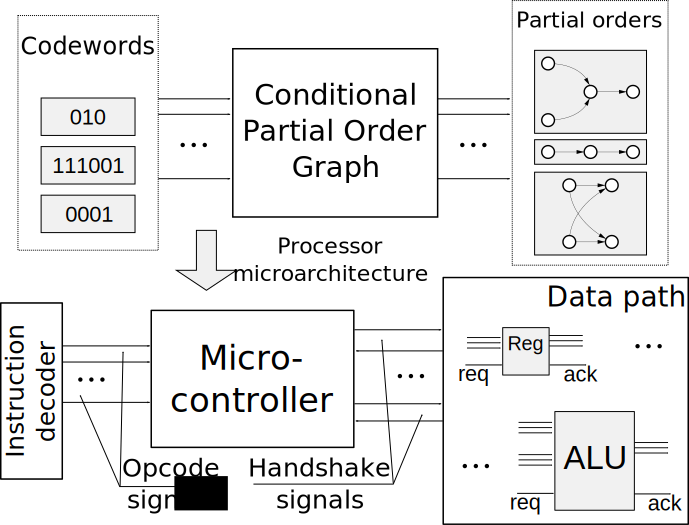
\includegraphics[width=0.6\columnwidth]{fig/control}\vspace{-1mm}

\par\end{centering}

\caption{CPOGs and processor microcontrol\label{fig:Dynamically-reconfigurable-controller}}
\vspace{-3mm}
\end{figure}


Synthesis of instruction sets is a particularly active research area.
There are methods for automated ISA synthesis for a target platform
(according to available system resources and data-path components)
and for given software requirements (e.g. aimed to ease compilation
or reduce program length). These methods eventually produce a structured
set of instructions satisfying certain properties (orthogonality,
completeness, regularity, etc.); instructions are grouped into classes
and each class is allocated a certain opcode interval within the total
code space~\cite{2003_nohl_dac}. At this point automation is typically
stopped or becomes trivial: the instructions are given arbitrary codes
within the allocated intervals. This limits performance due to instruction
decoder circuitry overheads. The problem is usually approached by
ad-hoc heuristics or application-specific optimisation techniques
(see, for example,~\cite{2002_lee_iccad}).

In this paper we try to solve the general problem of optimal encoding
of a given set of instructions with the aid of the Conditional Partial
Order Graph (CPOG) model introduced recently~\cite{2009_mokhov_phd}\cite{2010_mokhov_ieee}.
The key features of the model are: ability to describe systems in
a compact functional form, and structural synthesis methods which
significantly improve performance of the whole design flow. These
features make the model very efficient for representation and management
of processor instruction sets in hardware and EDA software. A CPOG
is a superposition of a set of partial orders which can be extracted
from it by providing the corresponding codewords, see Figure~\ref{fig:Dynamically-reconfigurable-controller}
(top). It can be regarded as a custom associative memory for storing
cause and effect relations within a predefined set of events.

There are different kinds of systems which can be described with the
model. For example, a processor microcontroller executes partial orders
(or \textbf{instructions}) of primitive computational steps (or \textbf{microinstructions})
defined on a set of data path operational units, see Figure~\ref{fig:Dynamically-reconfigurable-controller}
(bottom). The order is determined by an \textbf{instruction}\textbf{\emph{
}}\textbf{code} --- a combination of logical conditions presented
to the controller by the environment~\cite{1994_de_micheli_book}.
To this end, the microcontroller can be seen as an entity which communicates
with two parts of the environment: one part is the source of condition
signals (an instruction decoder) and the other part is a set of controlled
objects with request-acknowledgement interface (data path operational
units which execute the microinstructions).

There are many criteria which determine the choice of a particular
processor architecture and influence design of an instruction set:
functionality, operation modes, resources, etc. In Section~\ref{sec-processor}
we study an example of an instruction set (a subset of \emph{MSP430}
processor~\cite{mspmanual}) implemented on a minimalistic hardware
platform. However, the main focus of this paper is optimal encoding
of processor instruction sets in the general architecture-independent
context. See~\cite{2011_mokhov_tr} for investigation of the architecture-level
reasoning using the CPOG model.

Main contributions of this paper are: firstly, it formulates several
instruction set encoding problems in terms of the CPOG model; secondly,
it presents the SAT characterisation of the problems leading to their
efficient automated solution; thirdly, it demonstrates application
of the CPOG methodology at different stages of a processor design
flow --- from architectural-level specification, design and behavioural
description of an instruction set to its encoding and synthesis of
the physical implementation of the microcontroller. The paper is organised
as follows. Section~\ref{sec:CPOG-model-essentials} briefly introduces
the CPOG model providing a ground for formulating a set of problems
of optimal instruction set encoding in Section~\ref{sec:Optimal-encoding-problem}.
A method for automated translation of the problems into SAT instances
is explained in Section~\ref{sec:SAT-formulation}. It is followed
by a processor design example in Section~\ref{sec-processor} and
conclusions.

\section{Machine-assisted formalisation of parametrised graphs}


Since parametrised graphs are likely to be applied in a safety-critical toolchain, it is imperative to attain a degree of confidence in its properties. Equally important is to convince prospective users that the techniques is sound and lives up to its promises. To fullfil this goal, it was decided to construct in a strict and controlled manner a complete formalisation of the PG formalism. The Agda system \cite{agda} was chosen for its expressive notation language and extensive support for machine-checked formal inference. Agda has enjoyed a notable success as the basis for the formalisation (case studies, success stories)

Says that Agda is LCF, what is LCF. What are the altrenatives: Isaballe/HOL, HOL-Light, ACL2, Coq, PVS, Nqthm. What the have achieved (the colouring problem, pentium div, ...)

compare to Maude (2 lines)

a small agda example: list 

explain why an alegbraic specification is better suited than a model-based (VDM, Z, B) or process based (CSP, CCS).


The new Parametrised Graphs  introducing the following features:
\begin{itemize}
\item{it lifts the assumption of graph acyclicity, allowing general graphs instead of partial orders;}
\item{it adds algebraic operations for combining existing specifications, thus achieving compositionality;}
\item{it axiomatically defines the equivalence relation on specifications, allowing for equivalence preserving transformations.}
\end{itemize}




\section{Petri Nets}\label{sec_pn_basic}

% ***************** Petri Net Basics ********************
A \emph{Petri net} is a 4-tuple $N=(P,T,W,M_N)$ where
$P$ is a finite set of \emph{places} and $T$ is a finite set of \emph{transitions}
with $P \cap T=\emptyset$,
$W: P\times T \cup T \times P \rightarrow \nat_0$ is the \emph{weight function,} and
$M_N$ is the \emph{initial marking}, where a \emph{marking} is a multiset of places,
\ie a function $P\rar\nat_0$ which assigns a number of \emph{tokens} to each place.
A Petri net can be considered as a bipartite graph with weighted arcs between places and transitions.
If necessary, we write $P_N$ etc.\ for the components of $N$ or $P'$ ($P_i$) etc.\ for the net $N'$ ($N_i$) etc.


% ***************** Preset, Postset ********************

The \emph{preset} of a place or transition $x$ is denoted as $\pre x$ and defined by
$\pre x\DEF\{y\in P\cup T\ |\  W(y,x)>0\}$,
the \emph{postset} of $x$ is denoted as $\post x$ and defined by
$\post x\DEF\{y\in P\cup T\ |\ W(x,y)>0\}$.
These notions are extended to sets as usual.
We say that there is an \emph{arc}
from each $y\in \pre x$ to~$x$.




% ***************** Enabledness, Reachable States ********************

A transition $t$ is \emph{enabled under a marking M}
if $\forall p\in \pre t:M(p)\geq W(p, t)$, which is denoted by $M\tfrs t$.
An enabled transition $t$ can \emph{fire} yielding a new marking $M'$,
written as $M\tfrs t M'$,
where $M'(p)=M(p)-W(p, t) + W(t,p)$, for all $p\in P$.
A transition sequence $\sigma=t_1\ldots t_n$ is \emph{enabled under a marking $M$} (yielding $M'$)
if $M\tfrs{t_1}M_1\tfrs{t_2}\ldots M_{n-1}\tfrs {t_n} M_n=M'$, and we
write $M\tfrs \sigma$, $M\tfrs \sigma M'$ resp.; $\sigma$ is called \emph{execution of $N$} if $M_N\tfrs \sigma$.
  The empty transition sequence $\lambda$ is  enabled under every marking.
$M$ is called \emph{reachable} if a transition sequence $\sigma$ with
$M_N\tfrs \sigma M$ exists.

$N$ is called \emph{bounded} if, for every reachable marking $M$ and every place $p$, $M(p)\leq k$ for some constant $k\in \nat$; if $k=1$, $N$ is called \emph{safe}. $N$ is bounded if and only if the set $\tfrs {M_N}$ of reachable markings is finite. In this thesis, we are mostly concerned with bounded Petri nets.

A place $p$ is \emph{implicit} if it can be deleted from the net
without changing the set of executions, and so an implicit place can be removed from the net without affecting its behaviour.\footnote{Note that an implicit place can cease to be implicit if another implicit place is removed first.}
Unfortunately, detecting
implicit places is expensive: the problem is \PSPACE-complete for safe and \EXPSPACE-complete for general Petri nets. A place $p$ is \emph{duplicate} if there is another place $p'$ with the same pre- and postsets whose initial marking does not exceed that of $p$. Duplicate places are implicit, and are cheap to detect.

\smallskip

An \emph{STG} is a tuple $N=(P,T,W,M_N,\I,\Ot,\ell)$ where
$(P,T,W,M_N)$ is a Petri net and $\I$ and $\Ot$  are disjoint
sets of \emph{input} and  \emph{output signals}. For
$\Sig=\I\cup\Ot$ being the set of all signals,
$\ell:T\rightarrow\Sig\times\{+,-\}\cup \{\lambda\}$ is the
\emph{labelling} function. $\Sig\times\{+,-\}$ or short
$\Sig\upd$ is the set of \emph{signal transitions}; its
elements are denoted  as $s^+$, $s^-$  resp.\ instead of
$(s,+)$, $(s,-)$ resp. A plus sign denotes that a signal value
changes from \emph{logical low} (written as 0) to \emph{logical
high} (written as 1), and a minus sign denotes the opposite
direction. We write $s\upd$ if it is not important or unknown
which direction takes place.

An STG can contain transitions labelled with $\lambda$, called
\emph{dummy} transitions, which do not correspond to any signal
change. \emph{Hiding a signal $s$} means to change the label of
all transitions labelled with $s\upd$ to $\lambda$. (The idea
of re-synthesis approach is to hide the signals used for
communication between components, which results in an STG with
fewer signals that often has a simpler implementation as a
circuit.) The labelling of an STG is called \emph{injective} if
for each pair of distinct non-dummy transitions $t$ and $t'$,
$\ell(t)\neq\ell(t')$.

\smallskip

Examples of STGs are shown in Figs.~\ref{fi-motivating-example1} and~\ref{fi-motivating-example2}.
Places are drawn as circles containing a number of tokens corresponding to the initial marking.
Unmarked places which have only one transition in their presets and postsets are
not drawn if the corresponding arcs have the weight~1; they are implicitly
given by an arc between these two transitions (and if such a place contains tokens, they are drawn on the arc itself). Transitions are drawn simply as their labels,
and the weight function is drawn as directed arcs $(x,y)$ whenever $W(x,y)\neq 0$ (and
labelled with $W(x,y)$ if $W(x,y)>1$).


\smallskip

% ********************** labels ***************************

We lift the notion of enabledness to transition labels: we write
$M\ifrs {\ell(t)}  M'$ if $M\tfrs t  M'$. This is extended to sequences
as usual -- deleting $\lambda$-labels automatically since $\lambda$
is the empty word; \ie $M\ifrs{s\upd}M'$ means that a sequence of
transitions fires, where one of them is labelled $s\upd$ while the
others (if any) are $\lambda$-labelled. A sequence
$\nu\in(\Sig\upd)^*$ is called a \emph{trace of a marking} $M$ if
$M\ifrs \nu$, and a \emph{trace} of $N$ if $M=M_N$. The \emph{language $L(N)$
of $N$} is the set of all traces of $N$.

\smallskip

The \emph{reachability graph} $\RG(N)$ of an STG $N$ is an arc-labelled
directed graph on the reachable markings of $N$ with $M_N$ as the root;
there is an arc from $M$ to $M'$ labelled $\ell(t)$ whenever
$M\tfrs {t} M'$. For bounded Petri nets and STGs, $\RG(N)$ can be seen as a finite automaton
(where all states are accepting), and $L(N)$ is the language of this
automaton.
Observe that automata with accepting states only can be
regarded as STGs (with the states as places, the initial state being the
only marked place, etc.); hence, all definitions for STGs also
apply to automata.

$N$ is \emph{deterministic} if $\RG(N)$
is a deterministic automaton: it contains no $\lambda$-labelled transitions
and there are no \emph{dynamic auto-conflicts,} \ie for each reachable marking $M$ and each signal transition $s\upd$
there is at most one $M'$ with $M \ifrs {s\upd} M'$. (Note that a deterministic STG
can have choices between different outputs, \eg an STG modelling
the standard arbiter is deterministic).

An STG with a set of all markings $S_2$ is said to \emph{simulate} another STG with 
a set of all markings $S_1$ iff there exist an 
$R \subset S_1 \times S_2$ such that $(M_{N 1},M_{N 2}) \in R$ and for any pair of markings 
$(M_1, M_2) \in R$, a label $l$ and a marking $M_1'$, $M_1\ifrs {l}  M_1'$ implies 
$M_2 \ifrs {l} M_2'$ for some $M_2'$. We call $R$ the witness of simulation. Now we can say that STGs $N_1$ and $N_2$ are \emph{bisimilar} iff $N_2$ simulates $N_1$ with witness $R$ and $N_2$ simulates $N_1$ with witness $R^{-1}$.

For deterministic STGs, language equivalence and bisimulation coincide, and the language can be taken as the semantics of such a specification. Unfortunately, the class of deterministic STGs is too restrictive in practice~\cite{KSV-08}, \eg:
\begin{itemize}
  \item using dummy transitions is often convenient in manual design;
  \item modelling OR-causality~\cite{ykklp96} as a safe STG requires non-determinism;
  \item hiding internal communication (and thus introducing dummy transitions) is a crucial step in re-synthesis.
\end{itemize}
Hence, one has to deal with non-deterministic STGs as well.

One might think that if $\RG(N)$ is non-deterministic, it can be \emph{determinised} (using well-known auto\-ma\-ta-the\-o\-re\-tic methods), \ie turned  into a language-equivalent deterministic
automaton with accepting states only; in particular, the resulting automaton will have no $\lambda$-arcs. Unfortunately, this is a bad idea, as shown in~\cite{KSV-08}, where the semantics of non-deterministic STGs was developed. It is based on the concept of \emph{output-determinacy,} which is a relaxation of determinism: An STG $N$ is \emph{output-determinate (OD)} if $M_N \ifrs {\nu}
M_1$ and $M_N \ifrs {\nu} M_2$ implies for every $x\in \Ot_N$ that
$M_1 \ifrs {x\upd}$ iff $M_2 \ifrs {x\upd}$.
It turns out that OD STGs are exactly the STGs which
have correct implementations according to the implementation relation introduced in~\cite{KSV-08}.
Hence, non-OD STGs are ill-formed, and in particular cannot be correctly implemented as
circuits. This shows that in general, \emph{the language is not a satisfactory semantics of
non-deterministic STGs;} in particular, \emph{synthesising the determinised reachability graph of a non-OD STG
will either fail or result in an incorrect circuit.} On the other hand, for the class of OD STGs~\cite{KSV-08} shows that their language
is an adequate semantics, and
implementation relation can be formulated purely in terms of the language.
An important property of OD STGs is that in them the enabledness of an output signal is a function of the trace, \ie given a trace $\nu$, the set of outputs by which $\nu$ can be extended is uniquely determined, even though there could be multiple executions corresponding to $\nu$.


\smallskip

In the following definition
of {\em parallel composition}~$\parallel$, see \eg~\cite{vowo02lncs}, we will have to
consider the distinction between input and output signals.
The idea of parallel composition is that the
composed systems run in parallel and synchronise on common actions
-- corresponding to circuits that are connected on the
wires corresponding to the signals.
Since a system controls its outputs, we cannot allow a signal to
be an output of more than one component; input signals, on the other
hand, can be shared.
An output signal of a component may be an input of
other components, and in any case it is an output of the composition.

The parallel composition of STGs $N_1$ and $N_2$ is defined if
$\Ot_1 \cap \Ot_2 = \emptyset$. If we drop this requirement, the
definition gives the {\em synchronous product} $N_1\times N_2$,
which is often useful. The place set of the composition is
the disjoint union of the place sets of the components; therefore,
we can consider markings of the composition (regarded as multisets)
as the disjoint union of markings of the components,
and we will also write such a marking $M_1 \dot{\cup} M_2$
of the composition as $(M_1, M_2)$. To define the transitions,  let
$A=(\I_1 \cup \Ot_1) \cap (\I_2 \cup \Ot_2)$ be the set of
common signals.
If \eg $s$ is an output of $N_1$ and an input of $N_2$,
then firing of $s\upd$ in $N_1$ is `seen' by
$N_2$, \ie it must be accompanied by firing of $s\upd$
in $N_2$. Since we do not know a priori which $s\upd$-labelled
transition of $N_2$ will fire together with some $s\upd$-labelled
transition of $N_1$, we have to allow for each possible
pairing.
Thus, the {\em parallel composition} $N = N_1 \parallel N_2$
is obtained from the disjoint union of $N_1$ and $N_2$ by
fusing
each $s\upd$-labelled transition $t_1$ of $N_1$
with each $s\upd$-labelled transition $t_2$ from $N_2$ if $s \in A$.
Such transitions are pairs and the firing $(M_1, M_2)\tfrs{(t_1,t_2) }(M_1', M_2')$ of $N$
corresponds to the firings $M_i\tfrs{t_i}M_i'$ in $N_i$, $i=1,2$; for an example
of a parallel composition, see Fig.~\ref{fig_parcom}.
More generally, we have $(M_1, M_2) \ifrs{\nu} (M_1', M_2')$ iff
$M_i \ifrs{\nu|_{N_i}} M_i'$ for  $i\in\{1,2\}$, where
$\nu|_{N_i}$ denotes the projection of the trace $\nu$ onto the signals of the STG ${N_i}$.
Hence, all reachable markings of $N$ have the form $(M_1, M_2)$,
where $M_i$ is a reachable marking of $N_i$, $i=1,2$.

Obviously, one can extend the notion of the parallel
composition to a finite family (or collection) $(C_i)_{i\in I}$ of
STGs as $\parallel_{i\in I} C_i$,
provided that no signal is an output signal of more than one of the
$C_i$. We will also denote the markings of such a composition
by $(M_1, \ldots,M_n)$ if $M_i$ is a marking of $C_i$ for
$i\in I=\{1,...,n\}$.
As above, $(M_1, M_2, \ldots, M_n) \ifrs{\nu} (M_1', M_2', \ldots, M_n')$ iff
$M_i \ifrs{\nu|_{C_i}} M_i'$ for all $i\in\{1,\ldots,n\}$.
It is easy to see that $C$ is deterministic if all $C_i$ are. However, this is not true for a composition of OD STGs, as the result, in general, can be non-OD in such a case.

A composition can also be ill-defined due to \emph{computation interference,} see \eg~\cite{eber92}.
Let $C\DEF\parallel_{i\in I}C_{i}$ be a composition of STGs. It is
\emph{free from computation interference (FCI)} if for every trace $\nu$ of $C$
the following holds: if $\nu|_{C_{j}}x^{\pm}$ is a trace of $C_{j}$
for some output $x$ of $C_{j}$, then $\nu|_{C}x^{\pm}$ is a trace
of $C$.

\begin{figure*}[t]
    \centering
    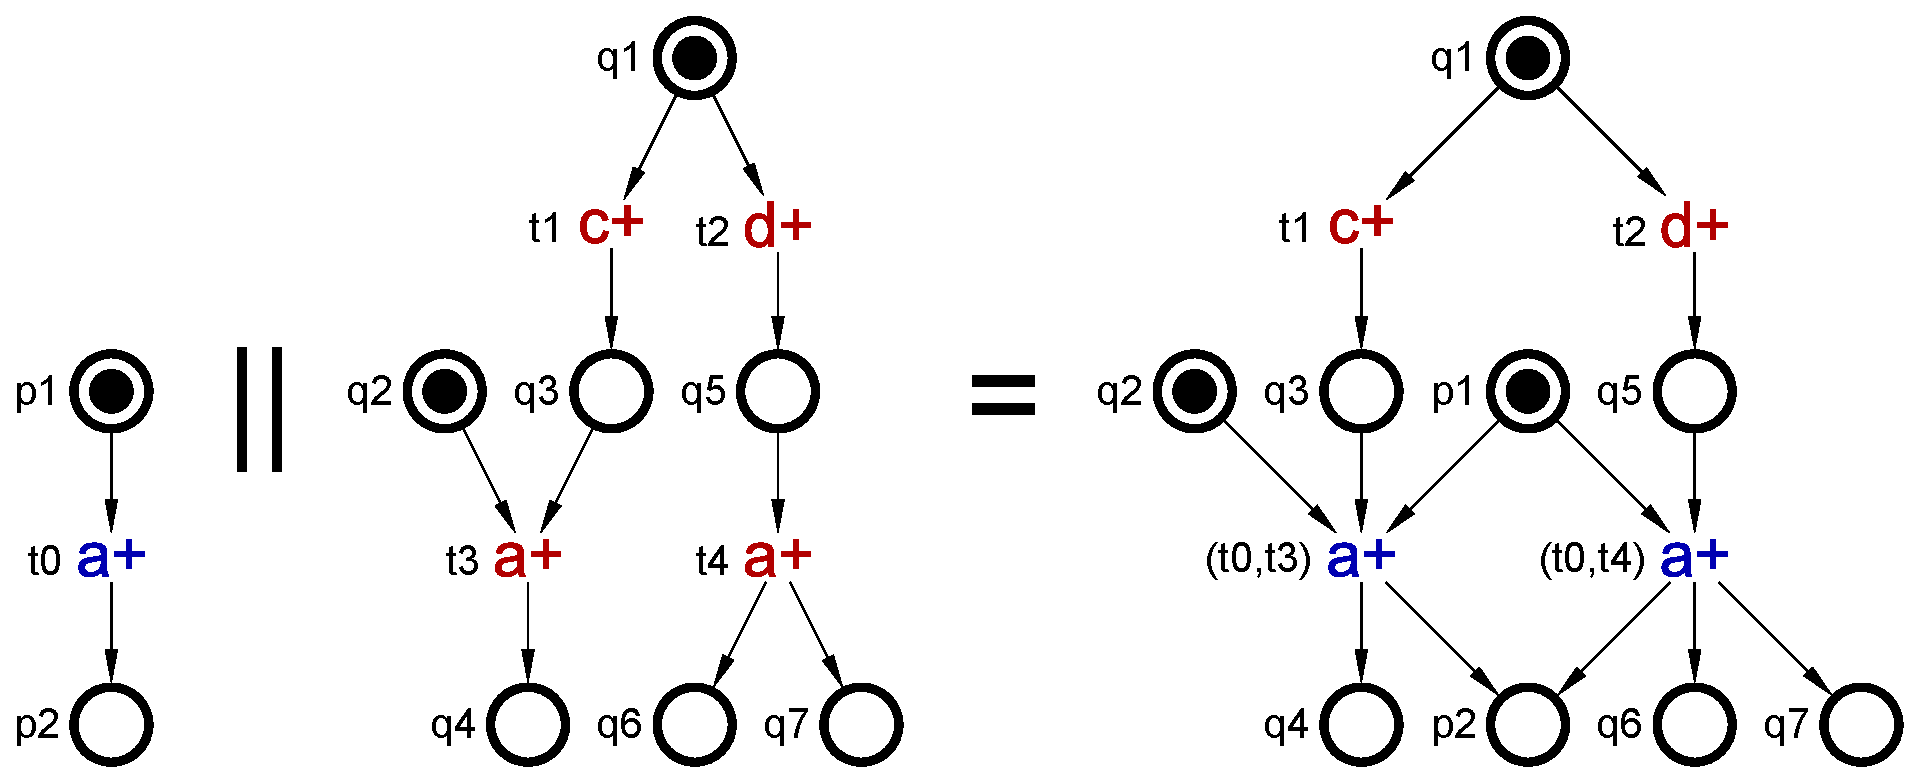
\includegraphics[scale=0.4]{EXPERIMENTS/stg/pcomp_example}
    \caption{\label{fig_parcom}
        Parallel composition example. In the net fragment on the left hand side,
        signal $a$ is an output, and in the fragment in the middle it is an input.
        Hence, in their parallel composition (right) it is an output.
        In this example, there is \emph{computation interference}: the left component activates $a\up$ but the middle one is not ready to receive it.}
\end{figure*}

\smallskip


\begin{figure*}[!tb]
    \centering
    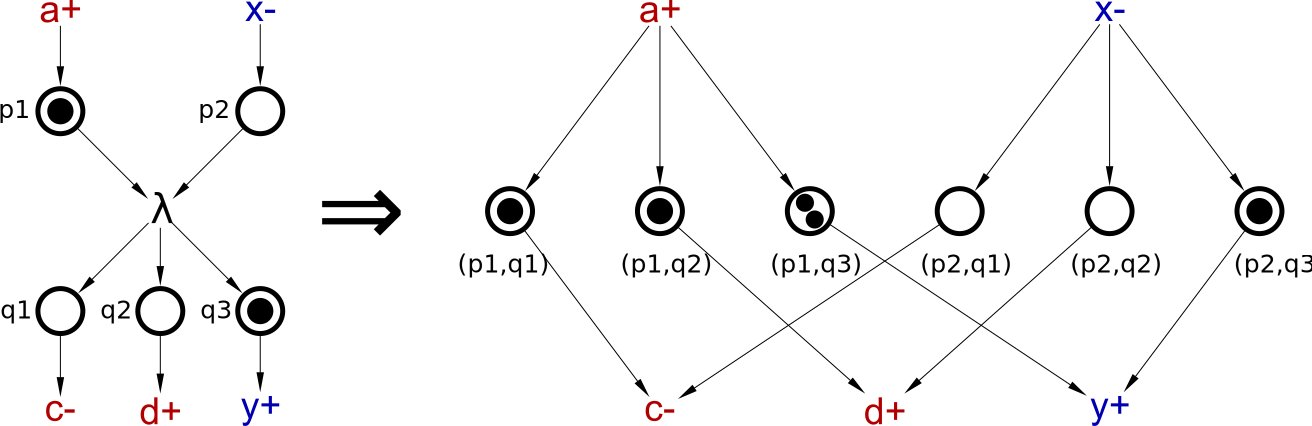
\includegraphics[scale=0.4]{EXPERIMENTS/stg/transition_contraction}
    \caption{\label{fig3.1}
        An example of a transition contraction.
    }
\end{figure*}


\emph{Transition contraction}~\cite{vowo02lncs} is an important operation in circuit re-synthesis. It removes a dummy transition from an STG and
combines each place of its preset with each place of its postset to `simulate' the
firing of the deleted transition, see Fig.~\ref{fig3.1}. Unfortunately, transition contractions are sometimes undefined (\eg in case the transition has a self-loop, \ie some place occurs in both its preset and postset); moreover, even when a contraction is defined, it might change the semantics of the STG.
Hence,~\cite{vowo02lncs} uses the notion of \emph{secure} contractions, that preserve the semantics.

Transition contractions preserve boundedness, but in general,
can turn a safe net into a non-safe one, as well as
introduce weighted arcs. In practice, it is often convenient to work with safe nets, and for this~\cite{KSVW-09} introduced \emph{safeness-preserving} contractions, \ie ones which
guarantee that  the transformed STG is safe if the initial one
was. (Note that the transitions with weighted arcs must be dead
in a safe Petri net, and so we can assume that the initial and
all the intermediate STGs contain no such arcs.) Also,~\cite{KSVW-09} developed a sufficient structural
condition for a contraction to be safe\-ness-pre\-ser\-ving.

From the point of view of this thesis, it is important to remark that implicit places can adversely affect the (secure) contractibility of a transition, \ie it is possible to have a situation when a transition is not contractible (or not securely contractible), but becomes securely contractible after some implicit place is removed from the STG. As detecting implicit places is expensive, it is very desirable to reduce their number by some other means, in particular the approach proposed in this thesis reduces the number of such places in STGs obtained by parallel composition. This has a direct effect on re-synthesis: if the composed STG has fewer implicit places, more dummy transitions in it can be contracted, and so it will be easier to synthesise the result.


\input{agda-processed-body}

%% \section{Redundancy in the Petri Nets produced by composition}

%% \section{Eliminating redundancy}

%% \section{Experimental results}

%% \section{Conclusions}

%% \chapter{CPOG Encoding}

\chapter{Processor instruction set encoding}

Main contributions of this chapter are: firstly, it formulates several
instruction set encoding problems in terms of the TPG model; secondly,
it presents the SAT characterisation of the problems leading to their
efficient automated solution; thirdly, it demonstrates application
of the TPG methodology at different stages of a processor design
flow --- from architectural-level specification, design and behavioural
description of an instruction set to its encoding and synthesis of
the physical implementation of the microcontroller. The chapter is organised
as follows. Section~\ref{sec:CPOG-model-essentials} briefly introduces
the CPOG model providing a ground for formulating a set of problems
of optimal instruction set encoding in Section~\ref{sec:Optimal-encoding-problem}.
A method for automated translation of the problems into SAT instances
is explained in Section~\ref{sec:SAT-formulation}. It is followed
by a processor design example in Section~\ref{sec-processor} and
conclusions.

\label{chap:PGEncoding}

The chapter is based on the results published in~\cite{cpog_encoding}. It shows how to represent processor instruction sets using CPOG formalism and provides
a ground for a concise formulation of several encoding problems, which
are reducible to the well-known Boolean satisfiability (SAT) problem
and can be efficiently solved by modern SAT solvers. Application of
all the presented techniques is demonstrated on a processor design
example.


\subsection{Criteria for optimality\label{sec:Criteria-for-optimality}}

A common measure of complexity of a Boolean formula $f$ is denoted
as $C(f)$ and is defined to be the total count of literals in it,
e.g. $C(x\cdot z+y\cdot\overline{z})=4$, $C(1)=0$, etc. 
This is the metric used in \cite{2009_mokhov_phd} to assess the produced encodings.
Indeed, when applied to a single formula this metric often works well:
the more literals the formula has, the larger the circuit to evaluate this formula.
However, when used to assess multiple similar formulae or a single formula with repeating sub-formulae,
this metric fails to account for the fact that the outputs of logic gates evaluating the subformulae
can be reused. To take advantage of this fact we use the new metric $G(C)$, showing the total number of
 gates in the circuit needed to compute all of the conditions found in $C$.
We use two versions of this metric, differing in type of gates allowed: one with AND/OR gates with 
all possible input and output inversions and another one with NAND-gates only.



\section{SAT formulation\label{sec:SAT-formulation}}

This section presents SAT formulations of the optimal encoding problems
described in the previous section.

The Boolean satisfiability problem (SAT) is to decide whether a given
Boolean formula $F(x_{1},\ x_{2},\ \dots,\ x_{n})$ is satisfiable
or not, i.e. if it is possible to find an assignment of Boolean values
$(\alpha_{1},\ \alpha_{2},\ \dots,\ \alpha_{n})\in\{0,\ 1\}^{n}$
to the variables $(x_{1},\ x_{2},\ \dots,\ x_{n})$ which makes the
formula true: $F(\alpha_{1},\ \alpha_{2},\ \dots,\ \alpha_{n})=1$.
As SAT is a decision (not optimisation) problem, we define a cost
function and use a binary search to minimise its value by calling
the SAT solver with different cost constraints.

We have implemented all the techniques presented in this section in
an automated software tool which uses \noun{MiniSAT}~\cite{2004_miniSAT_lncs}
as a SAT solver engine. \noun{MiniSAT} operates on CNF (conjunctive
normal form) representations of Boolean formulae. Since our SAT-instances
are not necessarily given in CNF, we implemented their automated conversion
to CNF formulae. This conversion introduces intermediate variables
but the overall size of the obtained formula is linear with respect
to the size of the given SAT-instance.



\subsection{Optimal encoding with unconstrained code length}

To solve the unconstrained optimal encoding problem described in Subsection~\ref{sec:Method-for-optimal}
we minimise the number of colours used for a conflict graph colouring.
Minimisation is performed by solving a series of instances of the
following decision problem.

Let $G=(V,\ E)$ be an extended conflict graph, where vertices $V$
correspond to encoding constraints and edges $E\subseteq V\times V$
to conflicts between them. $V$ contains both original $V_{o}=\{\mathbf{e}_{1},\ \mathbf{e}_{2},\ \dots,\ \mathbf{e}_{n}\}$
and inverted $V_{i}=\{\mathbf{\overline{\mathbf{e}}}_{1},\ \mathbf{\overline{\mathbf{e}}}_{2},\ \dots,\ \mathbf{\overline{\mathbf{e}}}_{n}\}$
constraints, such that $V=V_{o}\cup V_{i}$. The problem is to find
a colouring of $G$ which uses no more than $m$ colours.

For every pair of vertices $(\mathbf{e}_{k},\ \mathbf{\overline{\mathbf{e}}}_{k})$
we introduce a Boolean variable $p_{k}$ and an integer number $c_{k}$
whose values have to be found by the SAT solver: $p_{k}$ indicates
which of the two vertices is coloured -- if $p_{k}=1$ (resp. $p_{k}=0$)
then $\mathbf{e}_{k}$ (resp. $\overline{\mathbf{e}}_{k}$) is coloured,
while $c_{k}$ represents the colour of the chosen vertex. 

The SAT problem $\mathcal{ENCODE}$ consists of four constraints:
\[
\mathcal{ENCODE}=\mathcal{NUM}\cdot\mathcal{COL}_{oo}\cdot\mathcal{COL}_{oi}\cdot\mathcal{COL}_{ii}
\]
where $\mathcal{NUM}$ restricts colours such that $0\le c_{k}<m$.
Encoding of numbers $c_{k}$ in Boolean domain can be different, for
example, if we use binary encoding we need $\left\lceil \log_{2}m\right\rceil $
bits for each $c_{k}$. Implementation of $\mathcal{NUM}$ depends
on the chosen encoding; its general form is:
\[
\mathcal{NUM}=\prod_{1\le k\le n}(0\le c_{k})\cdot(c_{k}<m)
\]
Constraints $\mathcal{COL}$ check that adjacent vertices are assigned
different colours:
\[
\mathcal{COL}_{oo}=\prod_{(\mathbf{e}_{j},\ \mathbf{e}_{k})\in E\cap(V_{o}\times V_{o})}(p_{j}\cdot p_{k})\Rightarrow(c_{j}\neq c_{k})
\]
\[
\mathcal{COL}_{oi}=\prod_{(\mathbf{e}_{j},\ \overline{\mathbf{e}}_{k})\in E\cap(V_{o}\times V_{i})}(p_{j}\cdot\overline{p_{k}})\Rightarrow(c_{j}\neq c_{k})
\]
\[
\mathcal{COL}_{ii}=\prod_{(\overline{\mathbf{e}}_{j},\ \overline{\mathbf{e}}_{k})\in E\cap(V_{i}\times V_{i})}(\overline{p_{j}}\cdot\overline{p_{k}})\Rightarrow(c_{j}\neq c_{k})
\]
If we assume that complexity of comparison operations over numbers
$c_{k}$ is $C$, then the overall complexity of $\mathcal{ENCODE}$
is $\Theta((|V|+|E|)\cdot C)$. In particular, in case of binary encodings%
\footnote{Formula $(a<b)$ for binary numbers comparison is $(a<b)=\overline{a_{0}}\cdot b_{0}+(a_{0}=b_{0})\cdot(a'<b')$
where $a'$ and $b'$ are obtained from $a$ and $b$ by removal of
their most significant digits ($a_{0}$ and $b_{0}$); the formula
is linear with respect to the lengths of $a$ and $b$.%
} the complexity is $\Theta((|V|+|E|)\cdot\log m)$. Depending on the
chosen number encodings, there are from $\Theta(|V|\cdot\log m)$
to $\Theta(|V|\cdot m)$ free variables.

If $L$ is the minimum value of $m$ for which formula $\mathcal{ENCODE}$
is satisfiable then the optimal encoding uses $L$ variables $X=\{x_{1},\ x_{2},\ ...,\ x_{L}\}$.
Values $p_{k}$ and $c_{k}$ which satisfy the formula are used to
resolve encoding constraints $\mathbf{e}_{k}$ in the following way:
if $p_{k}=1$ then $\mathbf{e}_{k}$ is resolved by $x_{c_{k}}$,
otherwise it is resolved by $\overline{x_{c_{k}}}$.


\subsection{Optimal encoding with constrained code length}

The constrained version of the optimal encoding problem (see Subsection~\ref{Sec:Generating-optimal-opcodes})
is significantly more complicated and computationally intensive. It
requires finding a set of Boolean functions of $L$ arguments (where
$L$ is the specified code length) and there are $2^{2^{L}}$ of them
-- it is impossible to explore search spaces of such magnitudes, e.g.
$2^{2^{8}}$ roughly equals to the number of atoms in the universe.
To cope with this, we reduce the search space to 2-argument Boolean
functions only. From the practical point of view this is justified
by the fact that most modern technology libraries contain only 2-
or 3-input logic gates anyway. Importantly, every complex function
can be represented as a composition of simpler ones, therefore our
approach can find any function, albeit at the cost of introducing
intermediate variables. This is similar to what actually happens during
technology mapping\emph{ }and\emph{ }logic decomposition\emph{ }of
functional components into hardware gates~\cite{2002_cortadella_book}\cite{1994_de_micheli_book}.

Formally, let $(\mathbf{e}_{1},\ \mathbf{e}_{2},\ \dots,\ \mathbf{e}_{n})$
be a set of encoding constraints defined in Subsection~\ref{sec:Method-for-optimal},
$S$ be the number of scenarios, and $L$ be the required code length.
We are looking for such a vector $(\psi_{1},\ \psi_{2},\ \dots,\ \psi_{S})$
of $L$-bit encodings and $n$ functions $F_{j},\ 1\le j\le n$ such
that $F_{j}(\psi_{k})=\mathbf{e}_{j}[k]$ for every scenario $1\le k\le S$
(unless $\mathbf{e}_{j}[k]$ is a don't care value).

We represent a set of functions $F$ as a combinational circuit consisting
of $G$ 2-input Boolean gates, where $G$ is the value to be minimised.
An output of the circuit can be taken directly from one of its inputs
or be produced by a gate. In addition, any output can be inverted:
\[
F_{j}(\psi)=\mathit{select}(Signals(\psi),\ \mathit{oSelector}_{j})\oplus\mathit{Inv}_{j}
\]


Here $Signals(\psi)$ is a function computing all circuit signals
including both circuit inputs (given by parameter $\psi$) and gate
outputs, $\mathit{oSelector}_{j}$ is the number indicating which
circuit signal is `connected' to the $j$-th circuit output, function
$\mathit{select(V,\ k)}$ selects $k$-th element from a given vector
$V$, and $Inv_{j}=1$ iff $j$-th circuit output is inverted. Implementation
of function $select(V,\ k)$ depends on the encoding of $k$ (we used
one-hot encoding in this case, which allows for simpler implementation).
Circuit signals are computed as follows:
\[
\begin{cases}
\mathit{Signals}(\psi) & =\mathit{Wires}_{G}(\psi)\\
\mathit{Wires}_{k}(\psi) & =\begin{cases}
\psi & \textrm{\,\,\ if}\, k=0\\
\mathit{Wires}_{k-1}(\psi)\circ\mathit{Gate}_{k}(\psi) & \textrm{\,\,\ if}\,0<k\le G
\end{cases}\\
\mathit{Gate}_{k}(\psi) & =\mathit{arg}_{1,k}(\psi)\cdot\mathit{arg}_{2,k}(\psi)\\
\mathit{arg}_{j,k}(\psi) & =select(\mathit{Wires}_{k-1}(\psi),\ \mathit{aSelector}_{j,k})\oplus\mathit{InvArg}_{j,k}
\end{cases}
\]
In other words, a set of wires is initially equal to the set of circuit
inputs $(\mathit{Wires}_{0}(\psi)=\psi)$ and then is iteratively
extended by appending $Gate_{k}$ to the previously computed set of
wires $Wires_{k-1}$. Eventually, after $G$ iterations we obtain
the set of all signals $\mathit{Signals}(\psi)=\mathit{Wires}_{G}(\psi)$.
Every $Gate_{k}$ corresponds to an AND gate with possible input inversions
(indicated by $\mathit{InvArg}_{0,k}$ and $\mathit{InvArg}_{1,k}$).
Its arguments are selected by $\mathit{aSelector}_{0,k}$ and $\mathit{aSelector}_{1,k}$
from the set of wires computed in the previous iteration. This guarantees
the absence of combinational loops.

As every signal in the circuit can be optionally inverted (by setting
$\mathit{Inv}_{j}=1$ or $\mathit{InvArg}_{j,k}=1$), the resultant
gate basis includes 8 logic gates: AND, OR, NAND, NOR, plus 4 other
gates, obtained from these by inversion of exactly one of their inputs
(they do not have commonly adopted names, apart, perhaps, from Boolean
implication $x\Rightarrow y$ which corresponds to OR($\overline{x}$,
$y$)). We have also investigated a simpler basis, consisting of only
NAND gates with no optional input inversions. The basis leads to smaller
search space and works faster, but, as expected, produces larger circuits
(see Figure~\ref{fig:Comparison-of-different} for a comparison of
two bases on a processor example). If the NAND basis is used then
free variables $\mathit{InvArg}_{j,k}$ can be dropped and the formulae
for $\mathit{Gate}_{k}(\psi)$ and $\mathit{arg}_{j,k}(\psi)$ should
be modified as follows: 
\[
\begin{cases}
\mathit{Gate}_{k}(\psi) & =\overline{\mathit{arg}_{1,k}(\psi)\cdot\mathit{arg}_{2,k}(\psi)}\\
\mathit{arg}_{j,k}(\psi) & =select(\mathit{Wires}_{k-1}(\psi),\ \mathit{aSelector}_{j,k})
\end{cases}
\]
We tried to extend the 8-gate basis by addition of gates XOR and XNOR
but on practical examples it did not bring any benefit in terms of
the number of used gates, while significantly increasing the computation
time (due to additional free variables $\mathit{IsXor_{k}}$ and more
complex $\mathit{Gate}_{k}(\psi)$ functions).

In case of the standard 8-gate basis the SAT solver has to assign
the following free variables: $\psi_{j}[k]$ ($1\le j\le S,\ 1\le k\le L$),
$Inv_{j}$ ($1\le j\le n$), $\mathit{InvArg}_{0,j}$ and $\mathit{InvArg}_{1,j}$
($1\le j\le G$). Also it has to find numbers $\mathit{oSelector}_{j}$
($1\le j\le n$), $\mathit{aSelector}_{0,j}$ and $\mathit{aSelector}_{1,j}$
($1\le j\le G$). All other variables are derived.

The SAT problem $\mathcal{ENCODE}$ consists of two constraints:
\[
\mathcal{ENCODE}=\mathcal{NUM}\cdot\mathcal{EVAL}
\]
 Constraint $\mathcal{NUM}$ restricts all the selectors to their
domains:
\begin{multline}
\mathcal{NUM}=\prod_{1\le j\le n}(1\le\mathit{oSelector}_{j})\cdot(\mathit{oSelector}_{j}\le L+G)\cdot \\ \cdot\prod_{{1\le j\le2\atop 1\le k\le G}}(1\le\mathit{aSelector}_{j,k})\cdot(\mathit{aSelector}_{j,k}<L+k)
\end{multline}
Constraint $\mathcal{EVAL}$ checks that the circuit outputs satisfy
the encoding constraints:
\[
\prod_{{1\le j\le n\atop 1\le k\le S}}(\mathbf{e}_{j}[k]\neq-)\Rightarrow(F_{j}(\psi_{k})\Leftrightarrow\mathbf{e}_{j}[k])
\]


If $G_{min}$ is the minimum value of $G$ for which formula $\mathcal{ENCODE}$
is satisfiable then the optimal encoding is obtained in vectors $\psi_{j}$
($1\le j\le S$), an encoding constraint $\mathbf{e}_{k}$ is resolved
by function $F_{j}(\psi)$, and the circuit which produces these functions
contains $G_{min}$ gates.

We tried binary and one-hot number encodings in our implementation.
In both cases the complexity of the formula is $\Theta(S\cdot G\cdot(G+L))$.
The number of free variables is $\Theta(S\cdot L+(G+n)\cdot C)$,
where $C$ is $\log(G+L)$ and $G+L$ for binary and one-hot encodings,
respectively. In practice, one-hot encoding proved to be more efficient
despite significantly larger number of free variables. This can be
explained by the fact that one-hot encoding leads to simpler constraints.


\subsection{Support for dynamic variables\label{sub:Support-for-dynamic}}

A lot of practical applications require the use of \emph{dynamic
variables}, i.e. such variables that can change their values during
execution of a partial order and affect its further execution flow~\cite{2009_mokhov_phd}.
An example of such application, a processor microcontroller, is discussed
in the next section.

Dynamic variables manifest themselves as encoding constraints with
non-constant elements, e.g. $\mathbf{e}=110y1\overline{y}$, which
means that in the fourth scenario the corresponding condition has
to evaluate to some dynamic variable $y$ and in the sixth scenario
it has to evaluate to $\overline{y}$. To compute the optimal encoding
with such non-constant constraints we have to modify the method from
the previous subsection in the following way.

Let $y$ be a dynamic variable. We generate formula $\mathcal{ENCODE}_{0}$
(resp. $\mathcal{ENCODE}_{1}$) using encoding constraints where $y$
is replaced by 0 (resp. 1). Note that the free variables in both formulae
have to be the same and we have to add $y$ into the set of circuit
inputs. Then we use the SAT solver to find an assignment that satisfies
$\mathcal{ENCODE}_{0}\cdot\mathcal{ENCODE}_{1}$. Interpretation of
the resulting assignment is the same apart from the added input signal
$y$. In case of more than one dynamic variable, the process should
be repeated for each of them. Potentially this leads to an exponential
explosion of the formula. Fortunately, the number of dynamic variables
is rather small in practice, thus the explosion is not dramatic.

It is still possible to avoid the explosion of the formula by conversion
of the problem into an instance of 2-QBF problem (a quantified Boolean
formula with two quantifiers~\cite{2004_ranjan_qbf}):
\[
\exists X\,\forall Y\ \mathcal{ENCODE}
\]
where $X$ represents the set of all free variables, and $Y$ stands
for the set of dynamic variables. However, conversion of a formula
into 2-QBF does not necessarily reduce the computation time needed
to find its satisfying assignment. Implementation of a tool based
on a 2-QBF solver is a subject of future work.

The next section demonstrates application of this technique in a processor
microcontroller design.


\section{Processor design example\label{sec-processor}
}

This section demonstrates application of the CPOG-based methodology
to specification and synthesis of processor microcontrollers, and
discusses the results of optimal instruction encoding methods presented
in the previous section. Specification of such a complex system as
a processor starts at the architectural level which helps to deal
with the system complexity by structural abstraction~\cite{1994_de_micheli_book}.
Numerous processor architectures have emerged since fundamental von
Neumann architecture\emph{~}\cite{1946_burks_architecture} and Harvard
architecture\emph{~}\cite{1946_aiken_calculator} were proposed.
The example processor is built on the basis of Harvard architecture;
however, the method for optimal encoding of instructions presented
here is applicable to both architectures, including their
numerous derivatives.

\begin{figure}
\begin{centering}
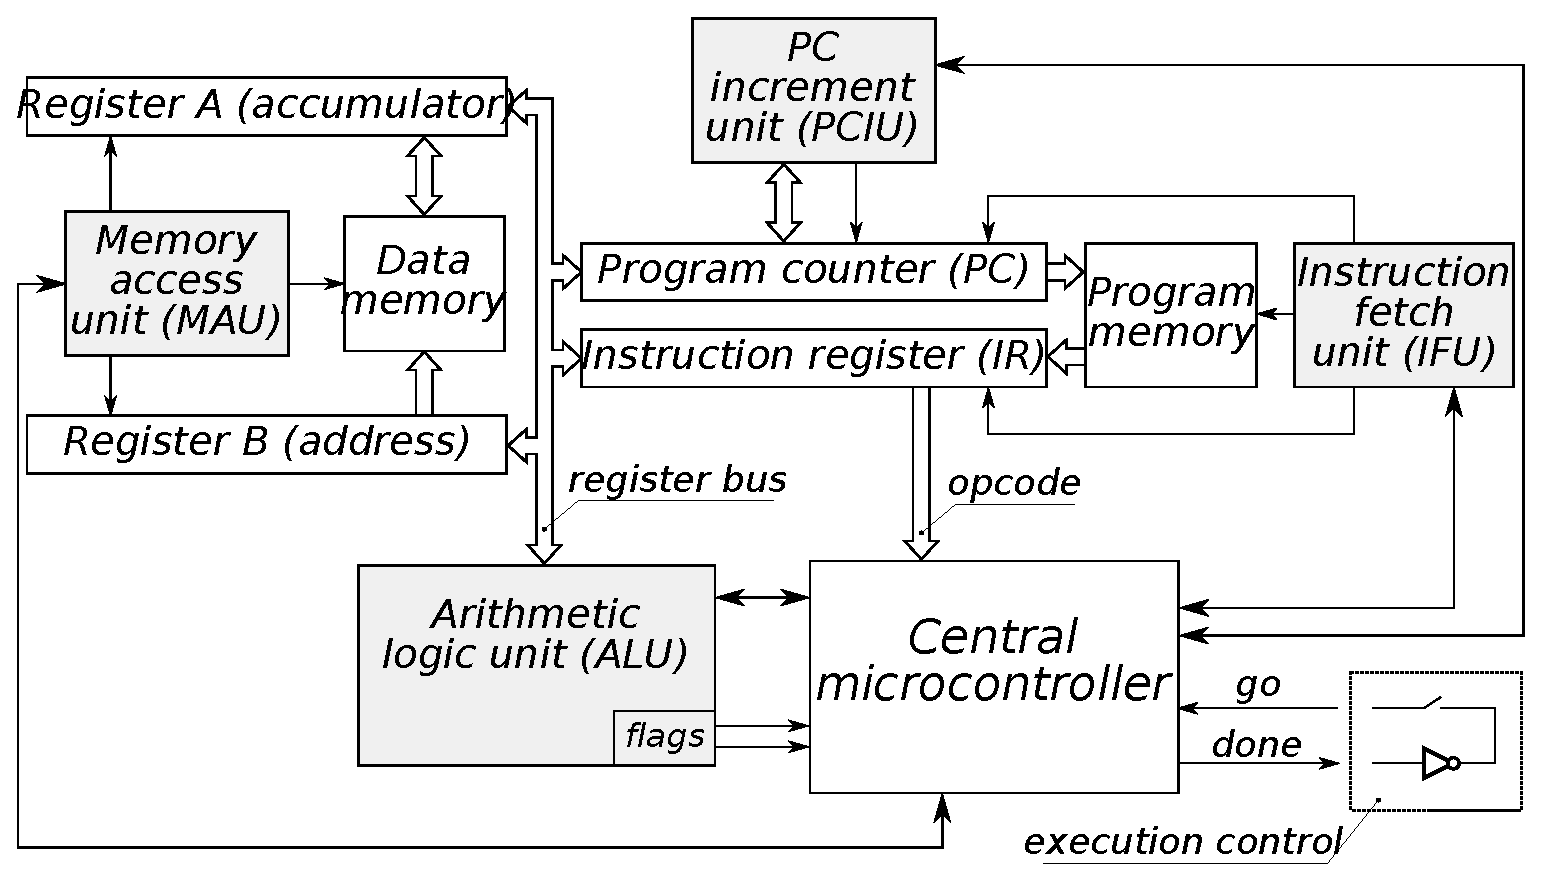
\includegraphics[width=0.75\columnwidth]{fig/processor_architecture}

\par\end{centering}

\caption{Architecture of example processor\label{app-fig-Architecture-of-example}}
\end{figure}



\subsection{Architecture}

Figure~\ref{app-fig-Architecture-of-example} shows the architecture
of the example processor. Separate \emph{Program memory} and \emph{Data
memory} blocks are accessed via \emph{Instruction fetch} (IFU) and
\emph{Memory access} (MAU) operational units, respectively. The
other two operational units are: ALU and \emph{Program counter increment
unit} (PCIU). The units are controlled via request-acknowledgement
interfaces (depicted as bidirectional arrows) by \emph{Central microcontroller}
which is our primary specification and synthesis objective. 

There are four registers: general purpose registers $A$ and $B$,
\emph{Program counter} (PC) which stores address of the current
instruction in the program memory, and \emph{Instruction register}
(IR) which stores opcode of the current instruction. For the purpose
of this example the actual width of the registers (the number of bits
they can store) is not important. ALU has access to all the registers
via the register bus; MAU accesses only general purpose registers;
IFU reads opcode of the next instruction into IR given its address
in PC; PCIU is responsible for incrementing PC (moving to the next
instruction). The microcontroller has access to the opcode and ALU
\emph{flags} (information about the current state of ALU which is
used in branching instructions).

\subsection{Dump 2}
This section demonstrates application of the CPOG-based methodology
to specification and synthesis of processor microcontrollers, and
discusses the results of optimal instruction encoding methods presented
in the previous section. Specification of such a complex system as
a processor starts at the architectural level which helps to deal
with the system complexity by structural abstraction~\cite{1994_de_micheli_book}.
Numerous processor architectures have emerged since fundamental von
Neumann architecture\emph{~}\cite{1946_burks_architecture} and Harvard
architecture\emph{~}\cite{1946_aiken_calculator} were proposed.
The example processor is built on the basis of Harvard architecture;
however, the method for optimal encoding of instructions presented
here is applicable to both architectures, including their
numerous derivatives.


\subsection{Architecture}

Figure~\ref{app-fig-Architecture-of-example} shows the architecture
of the example processor. Separate \emph{Program memory} and \emph{Data
memory} blocks are accessed via \emph{Instruction fetch} (IFU) and
\emph{Memory access} (MAU) operational units, respectively. The
other two operational units are: ALU and \emph{Program counter increment
unit} (PCIU). The units are controlled via request-acknowledgement
interfaces (depicted as bidirectional arrows) by \emph{Central microcontroller}
which is our primary specification and synthesis objective. 

There are four registers: general purpose registers $A$ and $B$,
\emph{Program counter} (PC) which stores address of the current
instruction in the program memory, and \emph{Instruction register}
(IR) which stores opcode of the current instruction. For the purpose
of this example the actual width of the registers (the number of bits
they can store) is not important. ALU has access to all the registers
via the register bus; MAU accesses only general purpose registers;
IFU reads opcode of the next instruction into IR given its address
in PC; PCIU is responsible for incrementing PC (moving to the next
instruction). The microcontroller has access to the opcode and ALU
\emph{flags} (information about the current state of ALU which is
used in branching instructions).


Now we have to define the set of instructions of the processor. Rather
than to list every single instruction it is easier to describe classes
of instructions with the same \emph{addressing mode}~\cite{mspmanual}
and partial order representation.

\textbf{ALU operation Rn to Rn}

An instruction from this class takes two operands stored in general
purpose registers $\{A,\ B\}$, performs an operation over them, and
writes the result back into one of them (so called \emph{register
direct addressing mode}). Examples: $\mathit{ADD\ A,\ B}$ -- addition
$A=A+B$; $\mathit{MOV\ B,\ A}$ -- assignment $B=A$. Figure~\ref{app-fig-Scenarios-of-8}(a)
shows the corresponding partial order of actions that have to be performed:
ALU works concurrently with PC increment (PCIU) and the next instruction
fetch (IFU) actions. As soon as both concurrent branches are completed,
the processor is ready to execute the next instruction. Note that
it is not important for the microcontroller which particular ALU operation
is being executed ($\mathit{ADD}$, $\mathit{MOV}$, or any other)
because the partial order of actions is not affected by this choice.
It is responsibility of ALU to detect which operation it has to perform
according to the current opcode. Therefore, it is sufficient to specify
only 8 behavioural scenarios of the microcontroller (as there are
8 classes of instructions).

\begin{figure}
\begin{centering}
\subfloat[ALU op. Rn to Rn]{

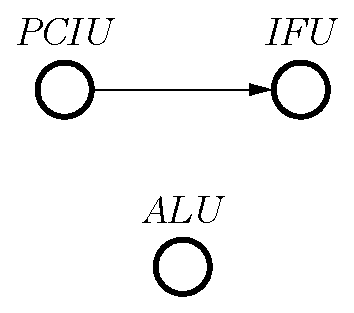
\includegraphics[scale=0.36]{fig/po_ALU_Rn_Rn}}\hfill{}\subfloat[ALU op. \#123 to Rn]{

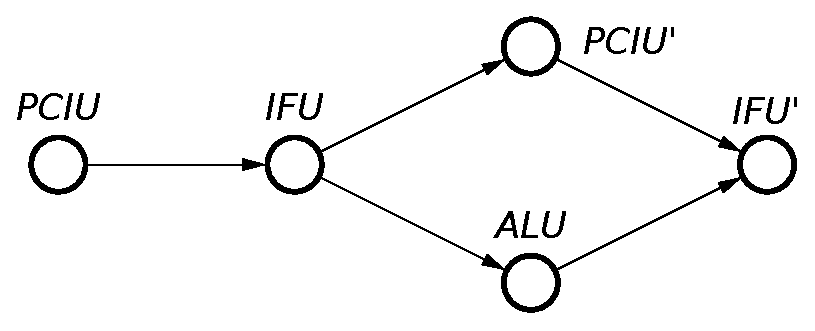
\includegraphics[scale=0.36]{fig/po_ALU_123_Rn}}\hfill{}\subfloat[ALU op. Rn to PC]{

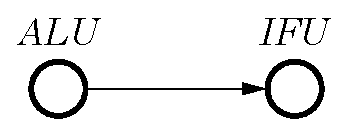
\includegraphics[scale=0.36]{fig/po_ALU_Rn_PC}}\hfill{}\subfloat[ALU op. \#123 to PC]{

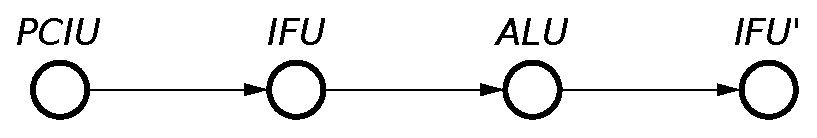
\includegraphics[scale=0.36]{fig/po_ALU_123_PC}}
\par\end{centering}

\begin{centering}
\subfloat[Memory access]{

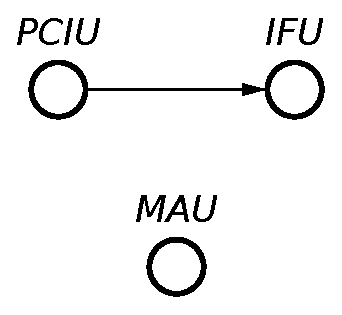
\includegraphics[scale=0.36]{fig/po_MAU}}\hfill{}\subfloat[Cond. ALU op. Rn to Rn]{

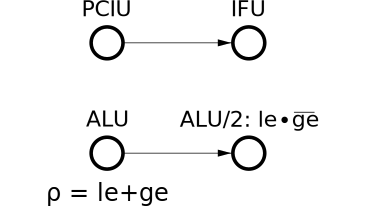
\includegraphics[scale=0.36]{fig/po_CALU_Rn_Rn}}\hfill{}\subfloat[Cond. ALU op. \#123 to Rn]{

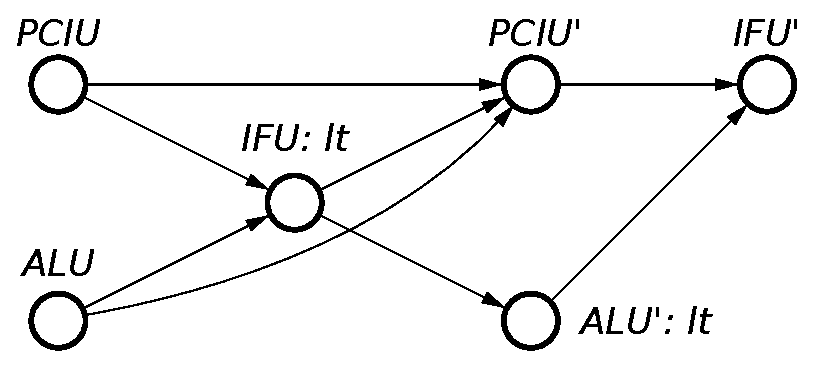
\includegraphics[scale=0.36]{fig/po_CALU_123_Rn}}\hfill{}\subfloat[Cond. ALU op. \#123 to PC]{

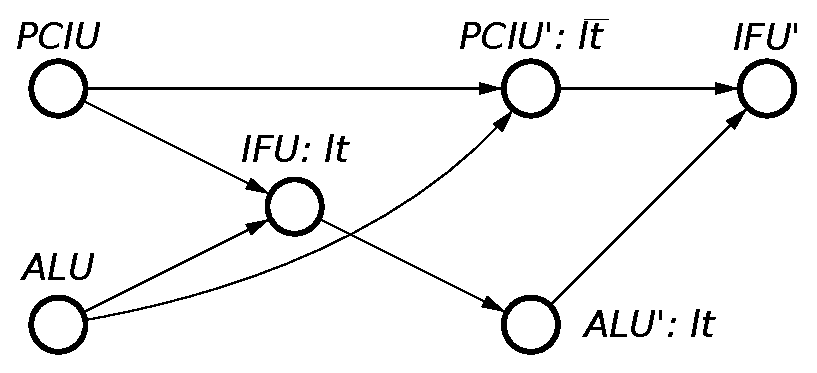
\includegraphics[scale=0.36]{fig/po_CALU_123_PC}}
\par\end{centering}

\caption{Conditional partial order specifications of 8 instruction classes\label{app-fig-Scenarios-of-8}}
\end{figure}


\textbf{ALU operation \#123 to Rn}

In this set of instructions one of the operands is register and another
is a constant which is given immediately after the instruction opcode
(e.g. $\mathit{SUB\ A,\ \#1}$ -- decrement $A$ by one), hence the
name: \emph{immediate addressing mode}. Figure~\ref{app-fig-Scenarios-of-8}(b)
shows the partial order of actions for such an instruction. At first,
the constant has to be fetched into IR (events PCIU and IFU). Then
ALU is executed concurrently with another increment of PC. Finally,
it is possible to fetch the next instruction into IR.

\textbf{ALU operation Rn to PC}

This class contains operations for unconditional branching, in which
PC register is modified. Branching can be absolute or relative: $\mathit{MOV\ PC,\ A}$
-- absolute branch to address stored in register $A$; $\mathit{ADD\ PC,\ B}$
-- relative branch to the address $B$ instructions ahead of the current
address. The partial order is very simple in this case: ALU is followed
with IFU -- see Figure~\ref{app-fig-Scenarios-of-8}(c).

\textbf{ALU operation \#123 to PC}

Instructions in this class are similar to those above with the exception
that the branch address is specified explicitly as a constant. The
actions should be scheduled in the following sequence: PCIU$\rightarrow$IFU
(to fetch the constant) followed by ALU and finally another IFU, as
shown in Figure~\ref{app-fig-Scenarios-of-8}(d).

\textbf{Memory access}

There are two instructions in this class: $\mathit{LOAD\ A}$ and
$\mathit{SAVE\ A}$. They load/save register $A$ from/to memory location
with address stored in register $B$. Figure~\ref{app-fig-Scenarios-of-8}(e)
shows that access to memory can be performed concurrently with the
next instruction fetch, exploiting the advantage of Harvard architecture.

\textbf{Conditional operations Rn to Rn, \#123 to Rn/PC}

These three classes of instructions are similar to their unconditional
versions above with the difference that they are performed only if
the following condition is true: $A<B$, i.e. register $A$ contains
a value which is less than that in register $B$. The first ALU action
compares registers $A$ and $B$, and changes ALU flags $\{le,\ ge\}$
according to the comparison result. These flags are thereafter checked
by the microcontroller in order to decide on the further scheduling
of actions. Consider, for example, conditional partial order in Figure~\ref{app-fig-Scenarios-of-8}(h).
It starts with concurrent increment of PC and comparison of registers
$A$ and $B$. If condition $A<B$ holds (i.e. $le\cdot\overline{ge}=1$)
then the process continues with the following sequence of actions:
IFU$\rightarrow$ALU/2$\rightarrow$IFU/2 (read the constant, perform
the branch, fetch the next instruction). Otherwise, the constant is
skipped (PCIU/2) and the next instruction is fetched (IFU/2). See~\cite{2009_mokhov_phd}
for details on dynamic CPOGs, which allow some of the operational
variables to be evaluated during execution of one of the scenarios
(in our case such dynamic variables are $\{le,\ ge\}$).






This section demonstrates application of TPG-algebra to designing
processor microcontrollers. Specification of such a complex system
as a processor has to start at the architectural level, which helps
to manage the system complexity by structural abstraction~\cite{1994_de_micheli_book}.

Fig.~\ref{app-fig-Architecture-of-example} shows the architecture
of an example processor. Separate \emph{Program memory} and \emph{Data
memory} blocks are accessed via the \emph{Instruction fetch} (IFU)
and \emph{Memory access} (MAU) units, respectively. The other two
operational units are: \emph{Arithmetic logic unit} (ALU) and \emph{Program
counter increment unit} (PCIU). The units are controlled using request-acknowledgement
interfaces (depicted as bidirectional arrows) by the\textbf{\emph{
}}\emph{Central microcontroller}, which is our primary design objective. 

The processor has four registers: two general purpose registers $A$
and $B$, \emph{Program counter} (PC) storing the address of the current
instruction in the program memory, and the \emph{Instruction register}
(IR) storing the \emph{opcode} (operation code) of the current instruction.
For the purpose of this chapter, the actual width of the registers (the
number of bits they can store) is not important. ALU has access to
all the registers via the register bus; MAU has access to general
purpose registers only; IFU, given the address of the next instruction
in PC, reads its opcode into IR; and PCIU is responsible for incrementing
PC (moving to the next instruction). The microcontroller has access
to the IR and ALU \emph{flags} (information about the current state
of ALU which is used in branching instructions).

Now we define the set of instructions of the processor. Rather than
listing all the instructions, we describe classes of instructions
with the same \emph{addressing mode}~\cite{mspmanual} and the same
execution scenario. As the scenarios here are partial orders of actions,
we use TPG-algebra, and the corresponding TPGs are shown in Fig.~\ref{app-fig-Scenarios-of-8}.

\textbf{ALU operation Rn to Rn}\quad{}An instruction from this class
takes two operands stored in the general purpose registers ($A$ and
$B$), performs an operation, and writes the result back into one
of the registers (so called \emph{register direct addressing mode}).
Examples: $\mathit{ADD\ A,\ B}$ -- addition $A:=A+B$; $\mathit{MOV\ B,\ A}$
-- assignment $B:=A$. ALU works concurrently with PCIU and IFU, which
is captured by the expression $\mathit{ALU}+\mathit{PCIU\rightarrow\mathit{IFU}}$;
the corresponding PG is shown in Fig.~\ref{app-fig-Scenarios-of-8}(a).
As soon as both concurrent branches are completed, the processor is
ready to execute the next instruction. Note that it is not important
for the microcontroller which particular ALU operation is being executed
($\mathit{ADD}$, $\mathit{MOV}$, or any other instruction from this
class) because the scenario is the same from its point of view (it
is the responsibility of ALU to detect which operation it has to perform
according to the current opcode). 


\begin{figure}
\begin{centering}
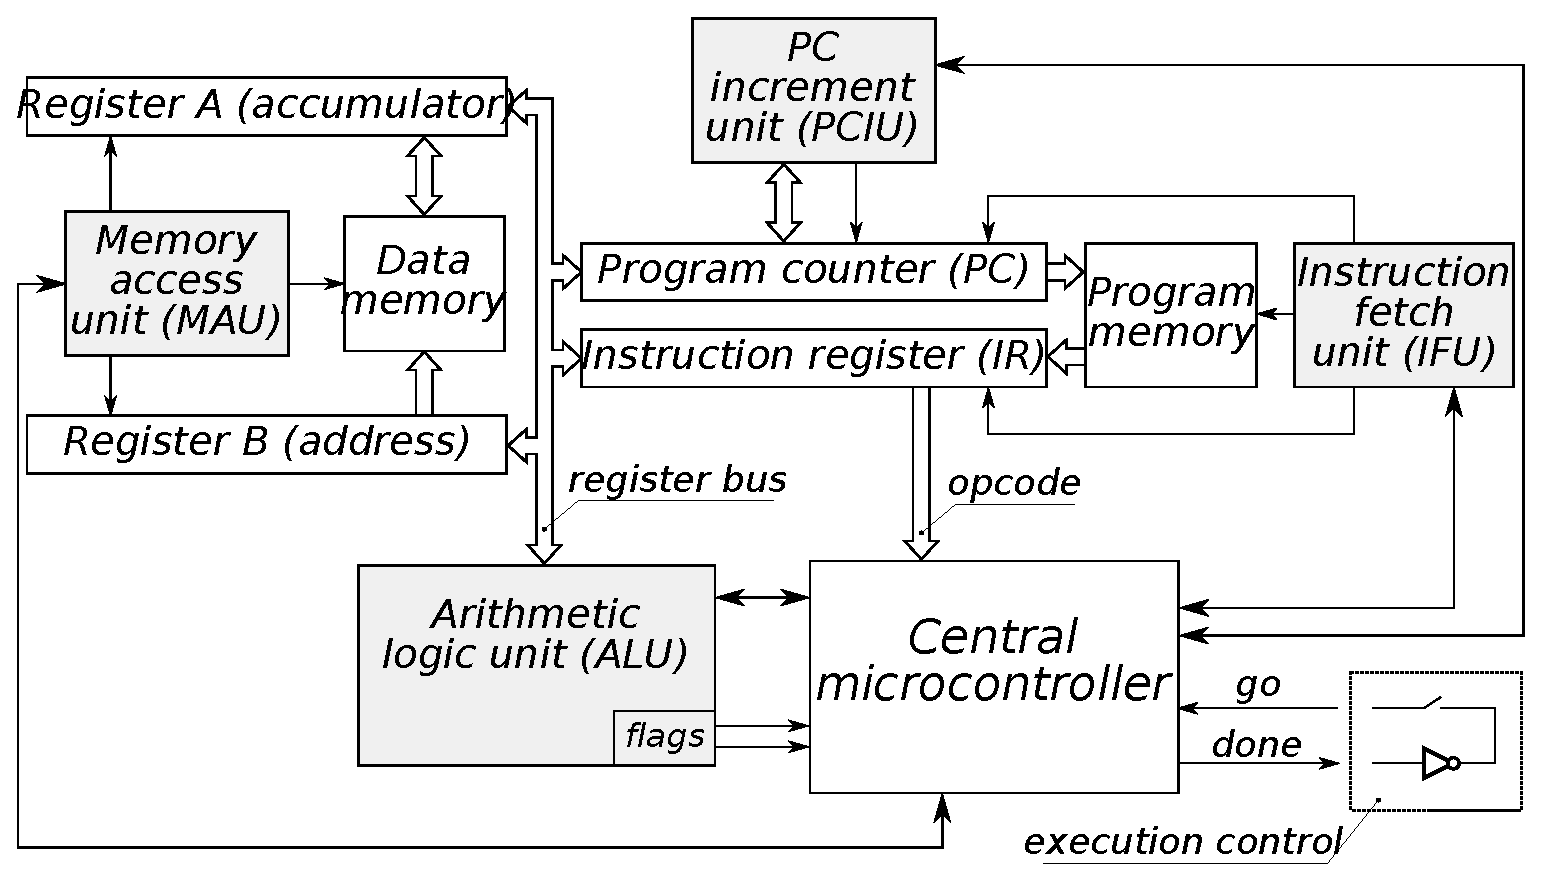
\includegraphics[width=1.04\columnwidth]{fig/processor_architecture}
\par\end{centering}
\caption{Architecture of an example processor\label{app-fig-Architecture-of-example}}
\vspace{-6mm}
\end{figure}


\begin{figure*}
\begin{centering}
\subfloat[ALU op. Rn to Rn]{

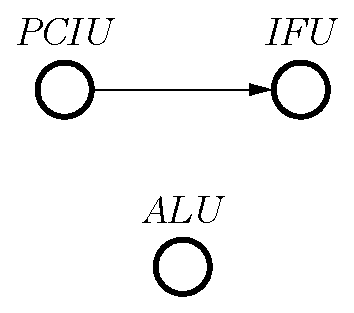
\includegraphics[scale=0.42]{fig/po_ALU_Rn_Rn}}\hfill{}\subfloat[ALU op. \#123 to Rn]{

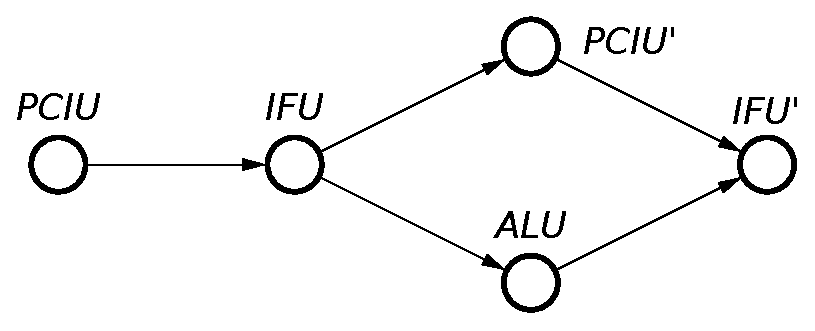
\includegraphics[scale=0.42]{fig/po_ALU_123_Rn}}\hfill{}\subfloat[ALU op. Rn to PC]{

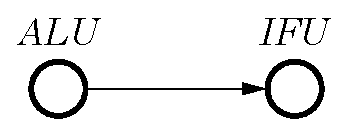
\includegraphics[scale=0.42]{fig/po_ALU_Rn_PC}}\hfill{}\subfloat[ALU op. \#123 to PC]{

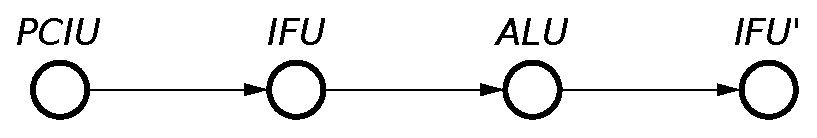
\includegraphics[scale=0.42]{fig/po_ALU_123_PC}}
\par\end{centering}

\begin{centering}
\subfloat[Memory access]{

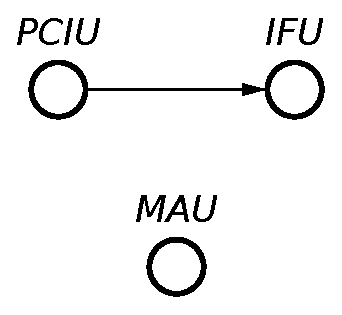
\includegraphics[scale=0.42]{fig/po_MAU}}\hfill{}\subfloat[Cond. ALU op. Rn to Rn]{

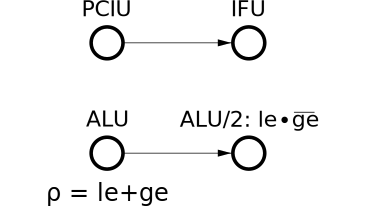
\includegraphics[scale=0.42]{fig/po_CALU_Rn_Rn}}\hfill{}\subfloat[Cond. ALU op. \#123 to Rn]{

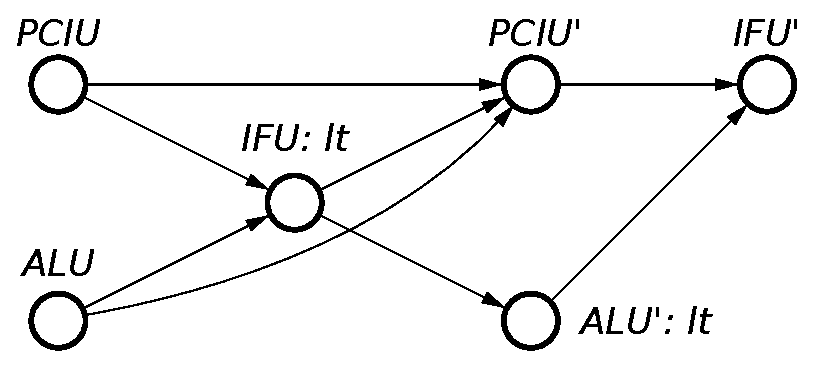
\includegraphics[scale=0.42]{fig/po_CALU_123_Rn}}\hfill{}\subfloat[Cond. ALU op. \#123 to PC]{

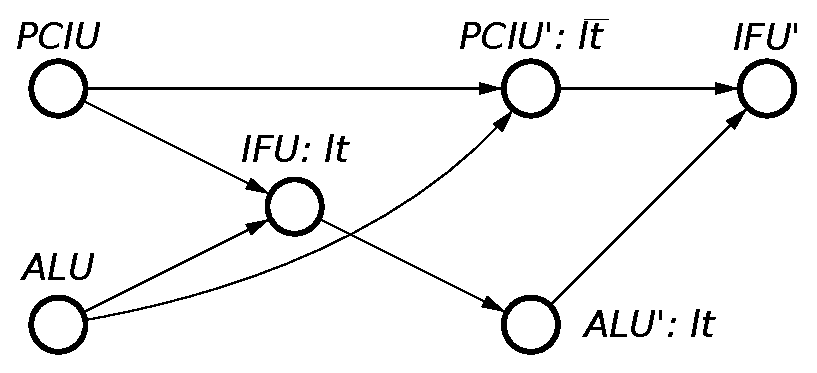
\includegraphics[scale=0.42]{fig/po_CALU_123_PC}}
\par\end{centering}

\caption{TPG specifications of instruction classes\label{app-fig-Scenarios-of-8}}
\vspace{-6mm}
\end{figure*}


\textbf{ALU operation \#123 to Rn}\quad{}In this class of instructions
one of the operands is a register and the other is a constant which
is given immediately after the instruction opcode (e.g. $\mathit{SUB\ A,\ \#5}$
-- subtraction $A:=A-5$), so called \emph{immediate addressing mode}.
At first, the constant has to be fetched into IR, modelled as $\mathit{PCIU}\rightarrow\mathit{IFU}$.
Then ALU is executed concurrently with another increment of PC: $\mathit{ALU}+\mathit{PCIU'}$
(we use $'$ to distinguish the different occurrences of actions of
the same unit). Finally, it is possible to fetch the next instruction
into IR: $\mathit{IFU'}$. The overall scenario is then $\mathit{PCIU}\rightarrow\mathit{IFU}\rightarrow(\mathit{ALU}+\mathit{PCIU'})\rightarrow\mathit{IFU'}$.

\textbf{ALU operation Rn to PC}\quad{}This class contains operations
for unconditional branching, in which PC register is modified. Branching
can be absolute or relative: $\mathit{MOV\ PC,\ A}$ -- absolute branch
to address stored in register $A$, $PC:=A$; $\mathit{ADD\ PC,\ B}$
-- relative branch to the address $B$ instructions ahead of the current
address, $PC:=PC+B$. The scenario is very simple in this case: $\mathit{ALU}\rightarrow\mathit{IFU}$.

\textbf{ALU operation \#123 to PC}\quad{}Instructions in this class
are similar to those above, with the exception that the branch address
or offset is specified explicitly as a constant. The execution scenario
is composed of : $\mathit{PCIU}\rightarrow\mathit{IFU}$ (to fetch
the constant), followed by an ALU operation, and finally by another
IFU operation, $\mathit{IFU'}$. Hence, the overall scenario is $\mathit{PCIU}\rightarrow\mathit{IFU}\rightarrow\mathit{ALU}\rightarrow\mathit{IFU'}$.

\textbf{Memory access}\quad{}There are two instructions in this class:
$\mathit{MOV\ A,\ [B]}$ and $\mathit{MOV\ [B],\ A}$. They load/save
register $A$ from/to memory location with address stored in register
$B$. Due to the presence of separate program and data memory access
blocks, this memory access can be performed concurrently with the
next instruction fetch: $\mathit{PCIU}\rightarrow\mathit{IFU}+\mathit{MAU}$.

\textbf{Conditional instructions}\quad{}These three classes of instructions
are similar to their unconditional versions above with the difference
that they are performed only if the condition $A<B$ holds. The first
ALU action compares registers $A$ and $B$, setting the ALU flag
$lt$ (less than) according to the result of the comparison. This
flag is then checked by the microcontroller in order to decide on
the further scheduling of actions. 

\textbf{Rn~to~Rn}\quad{}This instruction conditionally performs
an ALU operation with the registers (if the condition does not hold,
the instruction has no effect, except changing the ALU flags). The
operation starts with an ALU operation comparing $A$ with $B$; depending
on the result of this comparison, i.e. the status of the flag $lt$,
the second ALU operation may be performed. This is captured by the
expression $\mathit{ALU}\rightarrow[lt]\mathit{ALU'}$. Concurrently
with this, the next instruction is fetched: $\mathit{PCIU}\rightarrow\mathit{IFU}$.
Hence, the overall scenario is $\mathit{PCIU}\rightarrow\mathit{IFU}+\mathit{ALU}\rightarrow[lt]\mathit{ALU'}$.

\textbf{\#123~to~Rn}\quad{}This instruction conditionally performs
an ALU operation with a register and a constant which is given immediately
after the instruction opcode (if the condition does not hold, the
instruction has no effect, except changing the ALU flags). We consider
the two possible scenarios:
\begin{itemize}
\item $A<B$ holds: First, ALU compares $A$ and $B$ concurrently with
a PC increment; since $A<B$ holds, the ALU sets flag $lt$ and the
constant is fetched to the instruction register: $(\mathit{ALU}+\mathit{PCIU})\rightarrow\mathit{IFU}$.
After that PC has to be incremented again, $\mathit{PCIU'}$, and
ALU performs the operation, $\mathit{ALU'}$. Finally, the next instruction
is fetched (it cannot be fetched concurrently with $\mathit{ALU'}$
as ALU is using the constant in IR): $(\mathit{ALU'}+\mathit{PCIU'})\rightarrow\mathit{IFU'}$.
\item $A<B$ does not hold: First, ALU compares $A$ and $B$ concurrently
with a PC increment; since $A<B$ does not hold, the ALU resets flag
$lt$ and the constant that follows the instruction opcode is skipped
by incrementing the PC: $(\mathit{ALU}+\mathit{PCIU})\rightarrow\mathit{PCIU'}$.
Finally, the next instruction is fetched: $\mathit{IFU'}$.
\end{itemize}
\begin{figure*}
\centering
\begin{tabular}{||c||||c||}
\hline 
{\small Instructions class} & {\small Opcode: $xyz$}\tabularnewline
\hline 
\hline 
{\small ALU Rn to Rn} & {\small 000}\tabularnewline
\hline 
{\small ALU \#123 to Rn} & {\small 110}\tabularnewline
\hline 
{\small ALU Rn to PC} & {\small 101}\tabularnewline
\hline 
{\small ALU \#123 to PC} & {\small 010}\tabularnewline
\hline 
{\small Memory access} & {\small 100}\tabularnewline
\hline 
{\small C/ALU Rn to Rn} & {\small 001}\tabularnewline
\hline 
{\small C/ALU \#123 to Rn} & {\small 111}\tabularnewline
\hline 
{\small C/ALU \#123 to PC} & {\small 011}\tabularnewline
\hline 
\end{tabular}

~\\
\vspace{5mm}
~\\

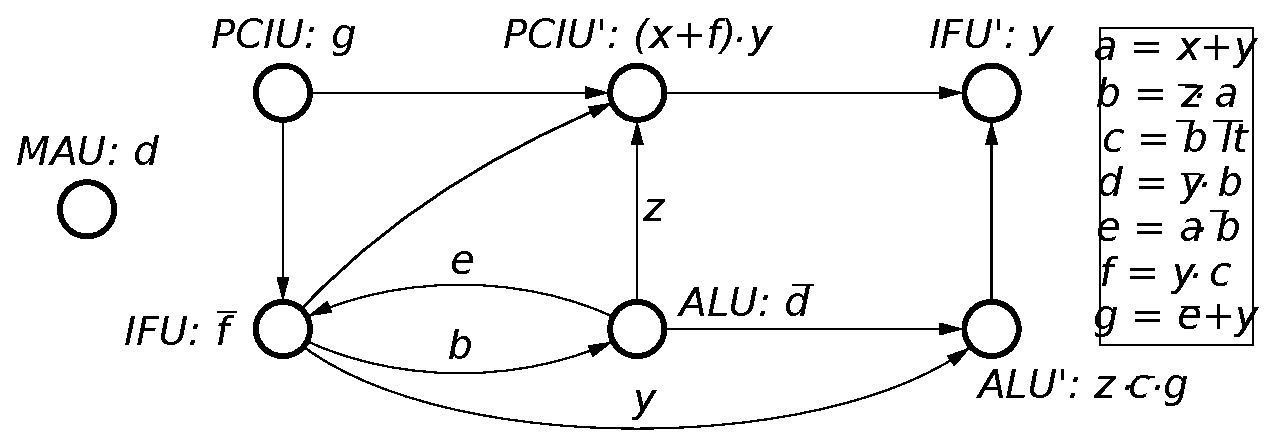
\includegraphics[scale=0.5]{fig/CPOG_L_3}

\caption{Optimal 3-bit instruction opcodes and the corresponding TPG specification
of the microcontroller\label{fig:opcodes-and-CG}}
\vspace{-6mm}
\end{figure*}


Hence, the overall scenario is the overlay of the two subscenarios
above prefixed with appropriate conditions (here we denote the predicate
$A<B$ by $lt$): 
\[
\begin{array}{c}
[lt]((\mathit{ALU}+\mathit{PCIU})\!\rightarrow\!\mathit{IFU}\!\rightarrow\!(\mathit{ALU'}+\mathit{PCIU'})\!\rightarrow\!\mathit{IFU'})+\\
+[\overline{lt}]((\mathit{ALU}+\mathit{PCIU})\!\rightarrow\!\mathit{PCIU'}\!\rightarrow\!\mathit{IFU'}).
\end{array}
\]
This expression can be simplified using the rules of TPG-algebra:%
\footnote{This case illustrates the advantage of using the new hierarchical
approach that allows to specify the system as a composition of scenarios
and formally manipulate them in an algebraic fashion. In our previous work~\cite{2011_mokhov_iet},
the CPOG for this class of instruction
was designed monolithically, and because of this the arc between $\mathit{ALU'}$
and $\mathit{IFU'}$ was missed. Adding this arc not only fixes the
dangerous race between these two blocks, but also leads to a smaller
microcontroller due to the additional similarity between TPGs for
this class of instructions and for the one described below.%
}
\[
(\mathit{ALU}+\mathit{PCIU})\!\rightarrow\![lt]\mathit{IFU}\!\rightarrow\!(\mathit{PCIU'}+[lt]\mathit{ALU'})\!\rightarrow\!\mathit{IFU'}.
\]


\textbf{\#123~to~PC}\quad{}This instruction performs a conditional
branching in which the branch address or offset is specified explicitly
as a constant. We consider the two possible scenarios:
\begin{itemize}
\item $A<B$ holds: First, ALU compares $A$ and $B$ concurrently with
a PC increment; since $A<B$ holds, the ALU sets flag $lt$ and the
constant is fetched to the instruction register: $(\mathit{ALU}+\mathit{PCIU})\rightarrow\mathit{IFU}$.
After that ALU performs the branching operation by modifying PC, $\mathit{ALU'}$.
After PC is changed, the next instruction is fetched, $\mathit{IFU'}$.
\item $A<B$ does not hold: the scenario is exactly the same as in the \textbf{\#123~to~Rn
}case when $A<B$ does not hold.
\end{itemize}
Hence, the overall scenario is the overlay of the two subscenarios
above prefixed with appropriate conditions (here we denote the predicate
$A<B$ by $lt$): 
\[
\begin{array}{c}
[lt]((\mathit{ALU}+\mathit{PCIU})\!\rightarrow\!\mathit{IFU}\!\rightarrow\!\mathit{ALU'}\!\rightarrow\!\mathit{IFU'})+\\
+[\overline{lt}]((\mathit{ALU}+\mathit{PCIU})\!\rightarrow\!\mathit{PCIU'}\!\rightarrow\!\mathit{IFU'}).
\end{array}
\]
This expression can be simplified using the rules of TPG-algebra:
\[
(\mathit{ALU}+\mathit{PCIU})\!\rightarrow\!([\overline{lt}]\mathit{PCIU'}+[lt](\mathit{IFU}\!\rightarrow\!\mathit{ALU'}))\!\rightarrow\!\mathit{IFU'}.
\]


The overall specification of the microcontroller can now be obtained
by prefixing the scenarios with appropriate conditions and overlaying
them. These conditions can be naturally derived from the instruction
opcodes. The opcodes can be either imposed externally or chosen with
the view to optimise the microcontroller. In the latter case, TPG-algebra
and TPGs allow for a formal statement of this optimisation problem
and aid in its solving; in particular, the sizes of the TPG-algebra
expression or TPG are useful measures of microcontroller complexity
(there is a compositional translation from a TPG-algebra expression
into a linear-size circuit). Note that it is natural to use three bits for opcodes as there
are eight classes of instructions, and give an example of optimal
3-bit encoding in the table in Fig.~\ref{fig:opcodes-and-CG}; the
TPG specification of the corresponding microcontroller is shown in
the right part of this figure (the TPG-algebra expression is not shown
because of its size).



\subsection{Instructions encoding}

Now the instructions have to be encoded. The simplest way to do this
is to use the binary encoding scheme, i.e. assign opcodes $\{000,\ \dots,\ 111\}$
to the instructions in arbitrary order as shown in Table~\ref{tab:Synthesised-instruction-codes}
(column `Trivial encoding'). This is not optimal in terms of area
and latency of the final microcontroller implementation. To obtain
the smallest possible CPOG specification one has to apply the optimal
encoding procedure from Section~\ref{sec:Method-for-optimal}. Generated
opcodes have 8 bits instead of 3 (shown in column `Optimal encoding'
of the same table). Whether 8 bit opcodes are affordable or not depends
on the chosen width of instruction register IR and other design parameters.
If it is not possible to use 8 bit opcodes one can try to apply the
constrained synthesis problem from Section~\ref{Sec:Generating-optimal-opcodes}
and generate instruction codes of required length $3\le L<8$ (it
is not possible to use less than 3 bits, and there is no sense in
setting $L\ge8$ because the optimal encoding uses 8 bits). We show
the generated opcodes for cases $L=3$ and $L=5$ -- see the corresponding
columns of Table~\ref{tab:Synthesised-instruction-codes}. Note that
the optimal 3-bit opcodes are very different from the trivial $000-111$
sequential encoding.

\begin{figure}[h]
\begin{centering}
\subfloat[Trivial encoding (35 literals)]{

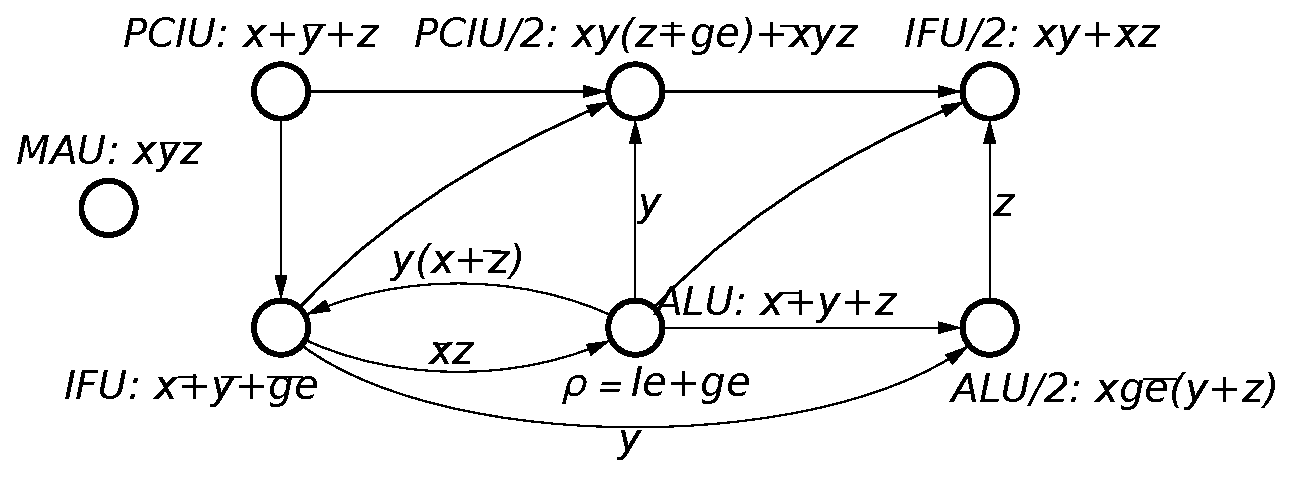
\includegraphics[scale=0.39]{fig/processor_cpog}}\hfill{}\subfloat[Optimal encoding (16 literals)]{

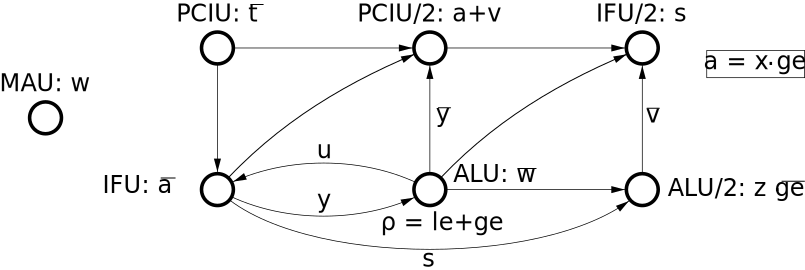
\includegraphics[scale=0.39]{fig/CPOG_L_8}}
\par\end{centering}

\begin{centering}
\subfloat[Optimal encoding $L=3$ (31 literals)]{

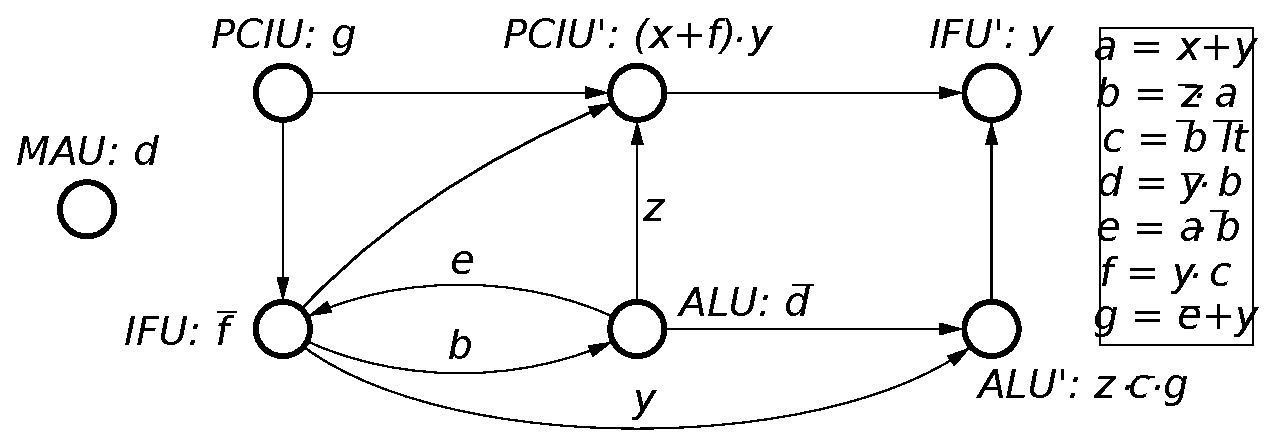
\includegraphics[scale=0.39]{fig/CPOG_L_3}}\hfill{}\subfloat[Optimal encoding $L=5$ (21 literals)]{

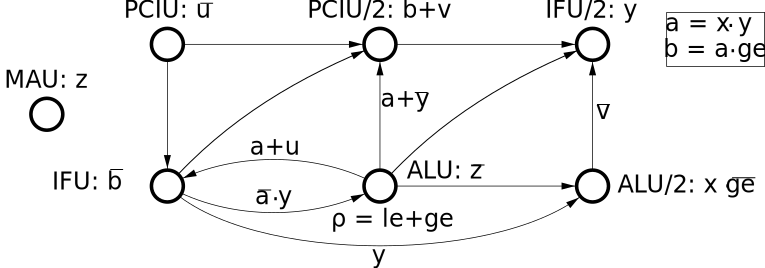
\includegraphics[scale=0.39]{fig/CPOG_L_5}}
\par\end{centering}

\caption{Synthesised CPOGs\label{fig:Synthesised-CPOGs}}
\end{figure}



\subsection{Microcontroller synthesis\label{app-sub-Microcontroller-synthesis}}

Figure~\ref{fig:Synthesised-CPOGs} shows four CPOGs obtained using
instruction encodings shown in Table~\ref{tab:Synthesised-instruction-codes}.
The trivial encoding results in the most complex CPOG shown in Figure~\ref{fig:Synthesised-CPOGs}(a);
it uses three variables $X=\{x,\ y,\ z\}$ and contains 35 literals.
The optimal encoding produces the CPOG with only 16 literals in its
conditions, Figure~\ref{fig:Synthesised-CPOGs}(b), but it uses 8
opcode variables $X=\{x,\ y,\ z,\ u,\ v,\ w,\ s,\ t\}$. Figures~\ref{fig:Synthesised-CPOGs}(c,
d) show the optimal CPOGs encoded with 3 and 5 ($X=\{x,\ y,\ z,\ u,\ v\}$)
variables, respectively; derived variables (denoted by names starting
from $a$) are shown in boxes.

\begin{figure}[h]
\begin{centering}
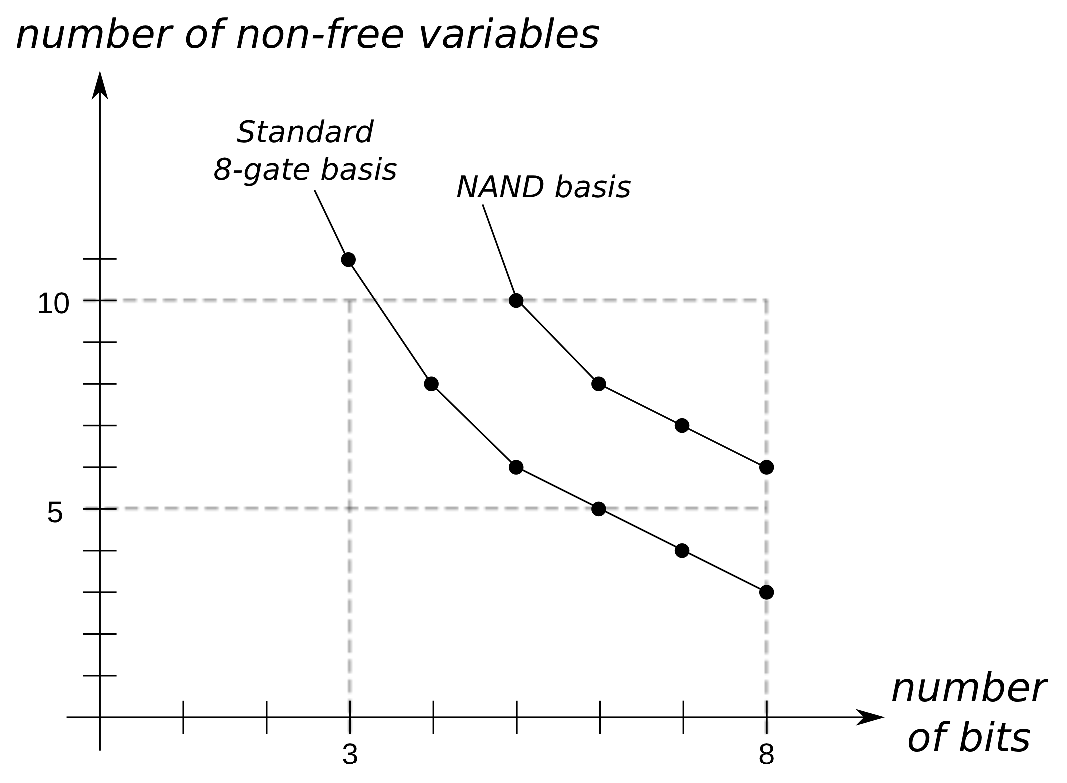
\includegraphics[scale=0.45]{fig/encoding_graph}
\par\end{centering}

\caption{Comparison of different gate bases\label{fig:Comparison-of-different}}
\end{figure}


Figure~\ref{fig:Comparison-of-different} illustrates dependency
of the number of non-free variables on the number of free variables.
As expected, the more free variables we have, the less non-free variables
are needed to satisfy all the encoding constraints. It is interesting
to note that if we restrict our functional basis to NAND gates only
(i.e. if we allow only functions $f_{k}=\overline{f_{i}\cdot f_{j}}$
to be used), the number of non-free variables does not increase dramatically.

Choice of a particular scenario within every CPOG in Figure~\ref{fig:Synthesised-CPOGs}
is highly distributed: every condition is responsible for rendering
only a little portion of the global picture and has a large don't
care set which leads to efficient Boolean minimisation. Note that
flag $le$ turned out to be redundant and was removed from all the
conditions, because original condition $le\cdot\overline{ge}$ is
equivalent to $\overline{ge}$ if the restriction function of ALU
($\rho_{ALU}=le+ge$) is satisfied: $\overline{ge}\cdot(le+ge)\Leftrightarrow le\cdot\overline{ge}$.
Thus it is enough to test only one ALU flag $ge$ to correctly schedule
all the instructions.

\begin{table}[b]
\begin{centering}
\begin{tabular}{|c||c|c|c||c|c|c|}
\hline 
Instructions class & $x$ & $z$ & $v$ & $\phi_{IFU}$ & $\phi_{ALU/2}$ & $\phi_{PCIU/2}$\tabularnewline
\hline 
\hline 
ALU Rn to Rn & 0 & 0 & 0 & 1 & 0 & 0\tabularnewline
\hline 
ALU \#123 to Rn & 0 & 0 & 1 & 1 & 0 & 1\tabularnewline
\hline 
ALU Rn to PC & 0 & 0 & 0 & 1 & 0 & 0\tabularnewline
\hline 
ALU \#123 to PC & 0 & 0 & 0 & 1 & 0 & 0\tabularnewline
\hline 
Memory access & 0 & 0 & 0 & 1 & 0 & 0\tabularnewline
\hline 
Cond. ALU Rn to Rn & 0 & 1 & 0 & 1 & $\overline{ge}$ & 0\tabularnewline
\hline 
Cond. ALU \#123 to Rn & 1 & 1 & 1 & $\overline{ge}$ & $\overline{ge}$ & 1\tabularnewline
\hline 
Cond. ALU \#123 to PC & 1 & 1 & 0 & $\overline{ge}$ & $\overline{ge}$ & $ge$\tabularnewline
\hline 
\hline 
Optimal condition & \multicolumn{3}{c|}{} & $\overline{x\cdot ge}$ & $z\cdot\overline{ge}$ & $x\cdot ge+v$\tabularnewline
\hline 
\end{tabular}
\par\end{centering}

\caption{Encoding of conditions with dynamic variable $ge$\label{app-tab-Encoding-of-non}}
\end{table}


The optimal CPOG (Figure~\ref{fig:Synthesised-CPOGs}(b)) contains
only 16 literals which leads to a twice smaller and faster microcontroller
than the one obtained using the trivial encoding. Note that in this
case it is not possible to reduce the final result to pure 1-restricted
form: the graph contains conditions depending on flag $ge$ which
cannot be mixed with other variables for optimisation purposes as
it is provided by ALU and can be changed during execution of an ALU
operation. Three non 1-restricted conditions are: $\phi(IFU)=\overline{a}=\overline{x\cdot ge}$,
$\phi(ALU/2)=z\cdot\overline{ge}$, and $\phi(PCIU/2)=a+v=x\cdot ge+v$.
It is impossible to use fewer literals for these conditions; this
is clarified in Table~\ref{app-tab-Encoding-of-non}: depending on
the instruction $\phi(IFU)$ has to evaluate either to $1$ or to
$\overline{ge}$ and this choice is delegated to operational variable
$x$ such that $\phi(IFU)=\overline{x\cdot ge}$. Condition $\phi(ALU/2)$
is similar: it must evaluate either to $0$ or to $\overline{ge}$,
hence $\phi(ALU/2)=z\cdot\overline{ge}$. The most complicated case
is presented with condition $\phi(PCIU/2)$ which has three possible
evaluations: $0$, $1$, and $ge$. Two variables are needed to handle
this leading to $\phi(PCIU/2)=x\cdot ge+v$. Optimal encoding of conditions
depending on ALU flags is performed automatically together with all
other conditions as explained in Subsection~\ref{sub:Support-for-dynamic},
thus the optimal result (in terms of the number of used literals)
is guaranteed.

Finally, the chosen CPOG can be mapped into equations to produce the
physical implementation of the microcontroller using the mapping algorithms
from~\cite{2009_mokhov_phd}\cite{2010_mokhov_ieee}.


% Encoding

% \section{The problem of choosing the optimal encoding}

% \section{Formulating the encoding problem as SAT problem}

% \section{Experimental results}

% \section{Conclusions}

% \chapter{Parametrised Graphs Algebra}

% Algebra

% \section{Generalising CPOGs}

% \section{Definitions}

% \section{Properties and their proofs}

% \section{Formally verified tools for PG formula manipulation}

% \section{Conclusions}

\chapter{Conclusions\label{chap:Conclusion}}

\section{Improved parallel composition}

We have presented an improved algorithm for computing the
parallel composition of STGs or labelled Petri nets. Under the
FCI assumptions, it allows to produce nets with fewer implicit
places, which aids the subsequent structural algorithms like
dummy contraction. It uses only simple structural checks and
thus is very efficient even for large compositions, so the
improvement comes at negligible cost.

The algorithm was implemented in the \pcomp tool and evaluated
on a set of scalable benchmarks. The experiments proved its
efficiency, which increases even more when the components are
pre-processed to remove dummies and ensure injective labelling
(this is usually cheap, as the components are small; moreover,
if the components come from a standard library of component
types, this step can be completely eliminated).

Another important advantage is that the improved algorithm
places almost no additional effort on the user: the only
requirement is to pass an additional command-line option to
\pcomp so that it can assume the FCI property and apply the
proposed optimisation.

\section{PG theory}

We introduced a new formalism called Parametrised Graphs and the
corresponding algebra. The formalism allows to manage a large number
of system configurations and execution modes, exploit similarities
between them to simplify the specification, and to work with groups
of configurations and modes rather than with individual ones. The
modes and groups of modes can be managed in a compositional way, and
the specifications can be manipulated (transformed and/or optimised)
algebraically in a fully formal and natural way.

We develop two variants of the algebra of parametrised graphs, corresponding
to the two natural graph equivalences: graph isomorphism and isomorphism
of transitive closures. Both cases are specified axiomatically, and
the soundness, minimality and completeness of the resulting sets of
axioms are formally proved. Moreover, the canonical forms of algebraic
terms are developed in each case.

The usefulness of the developed formalism has been demonstrated on
two case studies, a phase encoding controller and a processor micro-controller.
Both have a large number of execution scenarios, and the developed
formalism allows to capture them algebraically, by composing individual
scenarios and groups of scenarios. The possibility of algebraical
manipulation was essential to obtain the optimised final specification
in each case.

The developed formalism is also convenient for implementation in a
tool, as manipulating algebraic terms is much easier than general
graph manipulation; in particular, the theory of term rewriting can
be naturally applied to derive the canonical forms.

In future work we plan to automate the algebraic manipulation of PGs,
and implement automatic synthesis of PGs into digital circuits. For
the latter, much of the code developed for the precursor formalism
of Conditional Partial Order Graphs (CPOGs) can be re-used. One of
the important problems that needs to be automated is that of simplification
of (T)PG expressions, in the sense of deriving an equivalent expression
with the minimum possible number of operators. Our preliminary research
suggests that this problem is strongly related to modular decomposition
of graphs~\cite{2005_McConnell_modular}.

We have formalised the definitions of algebra of parametrised graph in Agda, and developed the machine-checked proofs of several properties of that algebra.

The formula representation data structure was designed together with the custom structural equivalence relation on formula representations for convenient formula manipulations. The equivalence relation has been proved equivalent to the one defined using formula semantics, thus showing its adequacy.

The normal form representation data structure for PG formulae was designed with its semantics defined as translation to the corresponding general formula representations.

The algorithm of finding the normal form of general formulae was developed and was proved to be correct.

The immediate future work includes formalising the proof of CPOG being a model of PG Algebra and modification of algorithm to compute the canonical form (where each graph node is mentioned no more than once) instead of just a normal form. Canonical form is much more useful because its size is at most quadratic while the size of a normal form is exponential in general.

The code used in this thesis is attached as an appendix.

\section{Processor instruction set encoding}

The Chapter~\ref{chap:PGEncoding} presented the PG model based methodology for micro architecture
design and studied its application for specification and synthesis
of a central processor microcontroller. The key contribution is
the method for synthesis of optimal instruction op-codes; the corresponding
optimisation problem is formulated in terms of PGs and reduced to
the well-known Boolean satisfiability problem. The method is implemented
in a software tool and can be used within the conventional micro architecture
design flow.

The studied processor example is purely academic. Nonetheless, it captures
many important features of real processors. It has been demonstrated
that the PG model is capable of modelling concurrency between different
subsystems and handling multiple choice during instruction execution.
Future work focuses on specification and synthesis of a real processor
and optimisation of the encoding algorithms.


\chapter*{Appendix}

What follows is the full Agda source code of formal proofs used in Chapter~\ref{chap:PGAlgebra}.

\input{agda-listing-body}

% \section{Workcraft framework plugin: Breeze handshake circuits}

% \section{Workcraft framework plugin: CPOG}

\section{Detailed proofs of PG Algebra properties}



\bibliographystyle{plain}
\bibliography{pg-algebra/danil,pg-algebra/publications,deco,pub,pg-encoding/publications,DATE10_Balsa/references}
\end{document}
